%!TeX encoding = UTF-8
%!TeX program = xelatex
\documentclass[
  notheorems,
  aspectratio=54,
]{beamer}

%% preamble
\title{An Introduction to Natural Language Processing}
% \subtitle{The subtitle}
\author{Jingsheng Gao}
\institute{Anqing Normal University}

\useoutertheme{shadow}
\setbeamertemplate{headline}{}
\mode<presentation>{
  \usetheme{Warsaw}
  \usecolortheme{seagull}
}

\setbeamertemplate{footline}
{
  \leavevmode%
  \hbox{%
  \begin{beamercolorbox}[wd=.45\paperwidth,ht=2.25ex,dp=1ex,center]{title in head/foot}%
    \usebeamerfont{title in head/foot}\inserttitle
  \end{beamercolorbox}%
  \begin{beamercolorbox}[wd=.45\paperwidth,ht=2.25ex,dp=1ex,center]{author in head/foot}%
      \usebeamerfont{author in head/foot}\insertauthor\ - \insertinstitute
  \end{beamercolorbox}%
  \begin{beamercolorbox}[wd=.1\paperwidth,ht=2.25ex,dp=1ex,right]{date in head/foot}%
    \insertframenumber{} / \inserttotalframenumber\hspace*{2ex} 
  \end{beamercolorbox}}%
  \vskip0pt%
}


\setbeamertemplate{navigation symbols}{}

\usepackage[
    backend=biber,
    autocite=superscript,
    sorting=none
]{biblatex}
\AtBeginBibliography{\small}
\addbibresource{refs.bib}

\usepackage{caption}
\captionsetup[figure]{font=scriptsize}

\usepackage{latexsym}
\usepackage{amsmath,amssymb}
\usepackage{mathtools}
\usepackage{color,xcolor}
\usepackage{graphicx}
\usepackage{algorithm}
\usepackage{amsthm}
\usepackage{lmodern}
% \usepackage[UTF8]{ctex}
% \usepackage{xeCJK}
\usepackage{animate} % insert gif

\usepackage{lipsum}
\usepackage{ulem}

\usepackage{listings} % display code on slides; don't forget [fragile] option after \begin{frame}

% ----------------------------------------------
% tikx
\usepackage{framed}
\usepackage{tikz}
\usepackage{pgf}
\usetikzlibrary{calc,trees,positioning,arrows,chains,shapes.geometric,%
    decorations.pathreplacing,decorations.pathmorphing,shapes,%
    matrix,shapes.symbols}

\usepackage{graphicx,wrapfig}
\usepackage[export]{adjustbox}



% ----------------------------------------------

% ---------------------------------------------------------------------
% Jet Black Theme
% \setbeamercolor{normal text}{fg=white,bg=black!90}
% \setbeamercolor{structure}{fg=white}
%
% \setbeamercolor{alerted text}{fg=red!85!black}
%
% \setbeamercolor{item projected}{use=item,fg=black,bg=item.fg!35}
%
% \setbeamercolor*{palette primary}{use=structure,fg=structure.fg}
% \setbeamercolor*{palette secondary}{use=structure,fg=structure.fg!95!black}
% \setbeamercolor*{palette tertiary}{use=structure,fg=structure.fg!90!black}
% \setbeamercolor*{palette quaternary}{use=structure,fg=structure.fg!95!black,bg=black!80}
%
% \setbeamercolor*{framesubtitle}{fg=white}
%
% \setbeamercolor*{block title}{parent=structure,bg=black!70!gray}
% \setbeamercolor*{block body}{fg=black,bg=black!10}
% \setbeamercolor*{block title alerted}{parent=alerted text,bg=black!15}
% \setbeamercolor*{block title example}{parent=example text,bg=black!15}
% ---------------------------------------------------------------------


% \newcommand{\reditem}[1]{\setbeamercolor{item}{fg=red}\item #1}

% \newcommand*{\Scale}[2][4]{\scalebox{#1}{\ensuremath{#2}}}

% -------------------------------------------------------------

% -------------------------------------------------------------

\begin{document}

% title frame
\begin{frame}
    \titlepage
\end{frame}

\newcommand{\subitem}[1]{
    {\fontsize{10}{12}\selectfont\setlength\itemindent{12pt} \item[+] #1}
}

\newcommand{\subsubitem}[1]{
    {\fontsize{10}{12}\selectfont\setlength\itemindent{40pt} \item[-] #1}
}

\begin{frame}{History}
  Natural language processing (NLP) is an interdisciplinary subfield of computer science and linguistics.
  \begin{itemize}
    \item Symbolic NLP (1950s – early 1990s)
    \item Statistical NLP (1990s–2010s)
    \item Neural NLP (present)
  \end{itemize}
\end{frame}

\begin{frame}{Common NLP tasks}
  \begin{itemize}
    \item Text and speech processing
      \subitem {Optical character recognition}
      \subitem {Speech recognition}
      \subitem {Text-to-speech}
    \item Lexical semantics (of individual words in context)
    \item Discourse (semantics beyond individual sentences)
    \item Higher-level NLP applications
      \subitem {Automatic summarization (text summarization)}
      \subitem {Natural-language generation (NLG)}
      \subitem {Question answering}
      \subitem {Machine translation (MT)}
  \end{itemize}
\end{frame}

\begin{frame}{Latest Approach}
 \begin{itemize}
    \item
      Transformers were developed to solve the problem machine translation and sequence transduction, or neural machine translation … but they do so much more!
      \subitem{Great performance in computer vision like ViT(Dosovitskiy, 2020)}
      \subitem{Image Classification (CoCa Transformer)}
      \subitem{Generative pre-trained transformers (GPT) are a type of large language model and are based on the transformer architecture.}
  \end{itemize}
\end{frame}


\begin{frame}{Previous Work}
  \begin{itemize}
    \item Pre-2014 - RNN, LSTM, GRU
       \subitem{RNNs struggled with long sequence data}
       \subitem{Could not handle long sequence lengths (forgetful)}
    \begin{figure}
      \centering
      \textbf{RNN}\par\medskip
      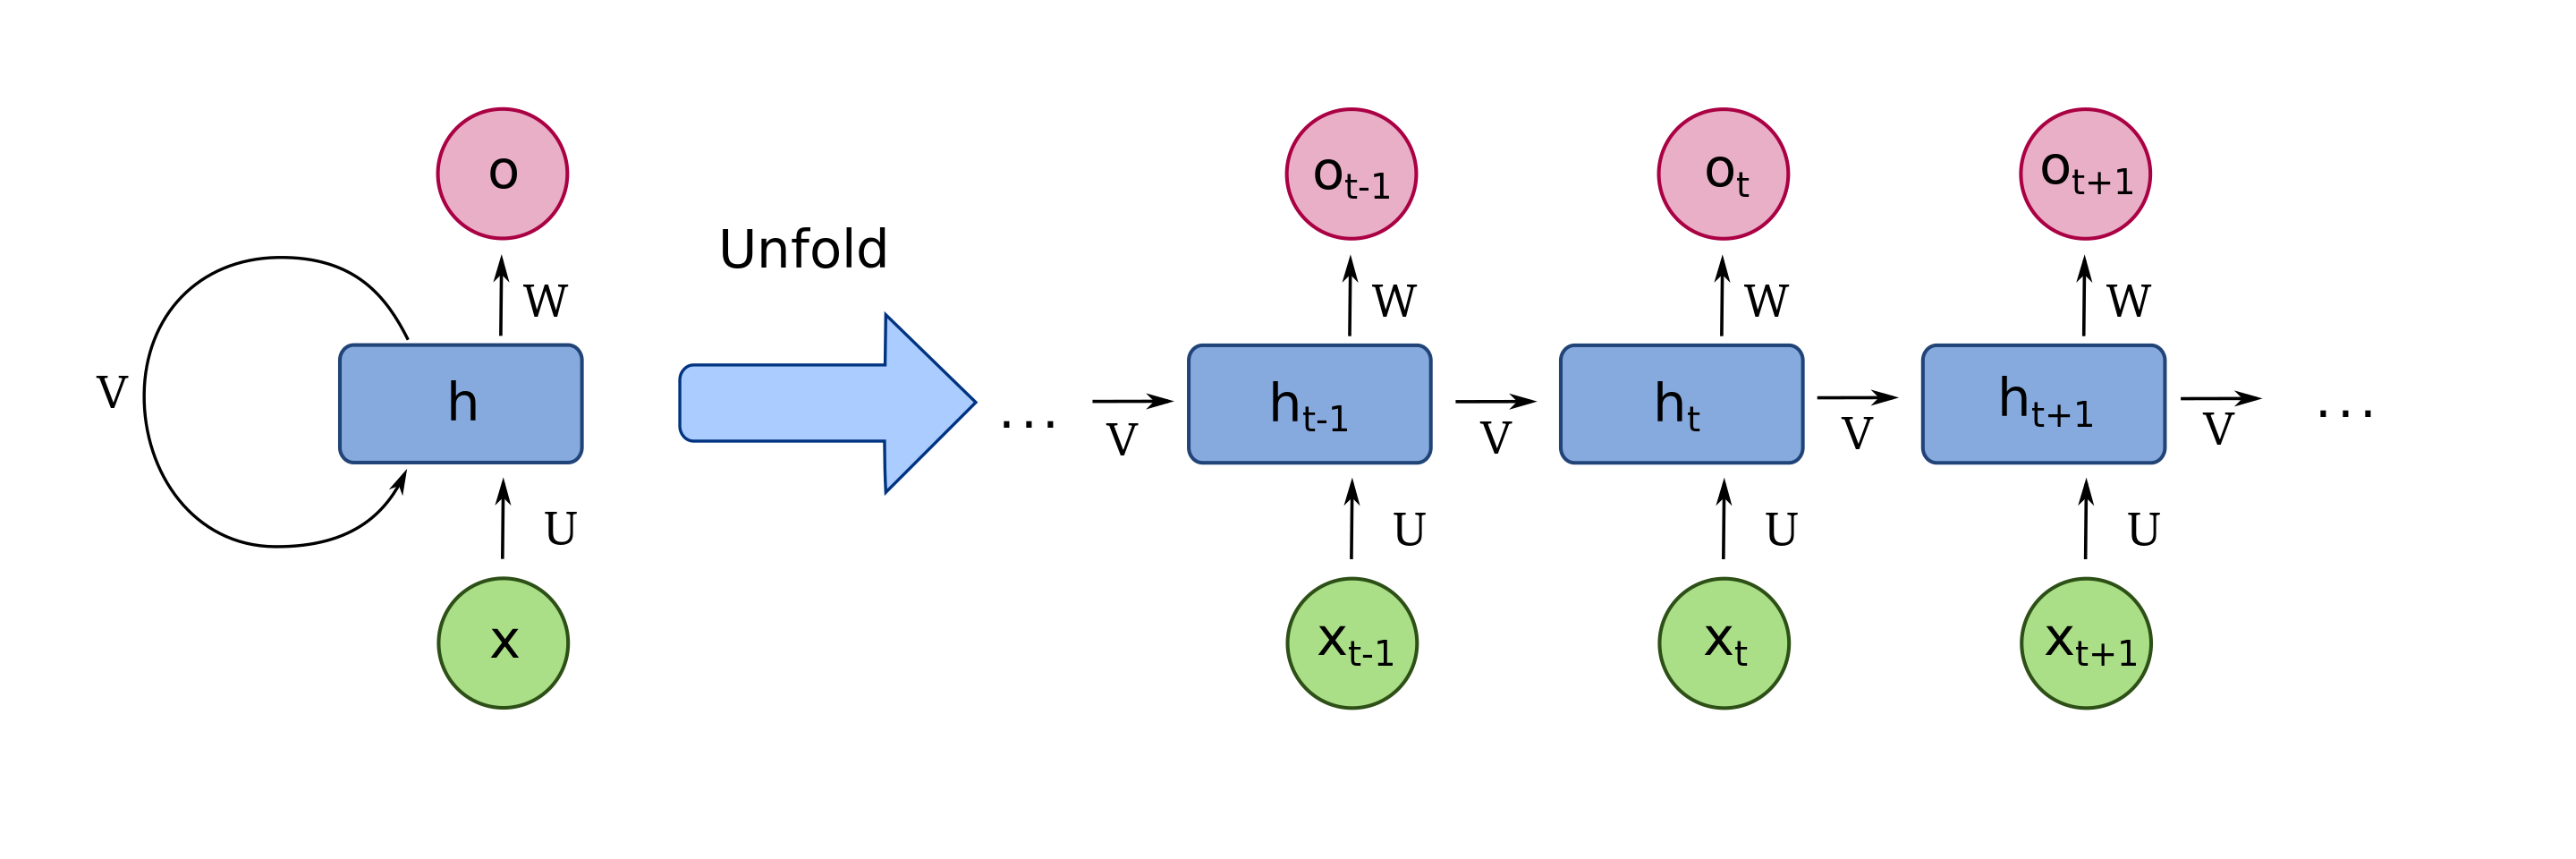
\includegraphics[width=0.6\textwidth]{rnn.png}
    \end{figure}
    \begin{figure}
      \begin{minipage}[b]{0.45\textwidth}
        \textbf{LSTM Cell}\par\medskip
          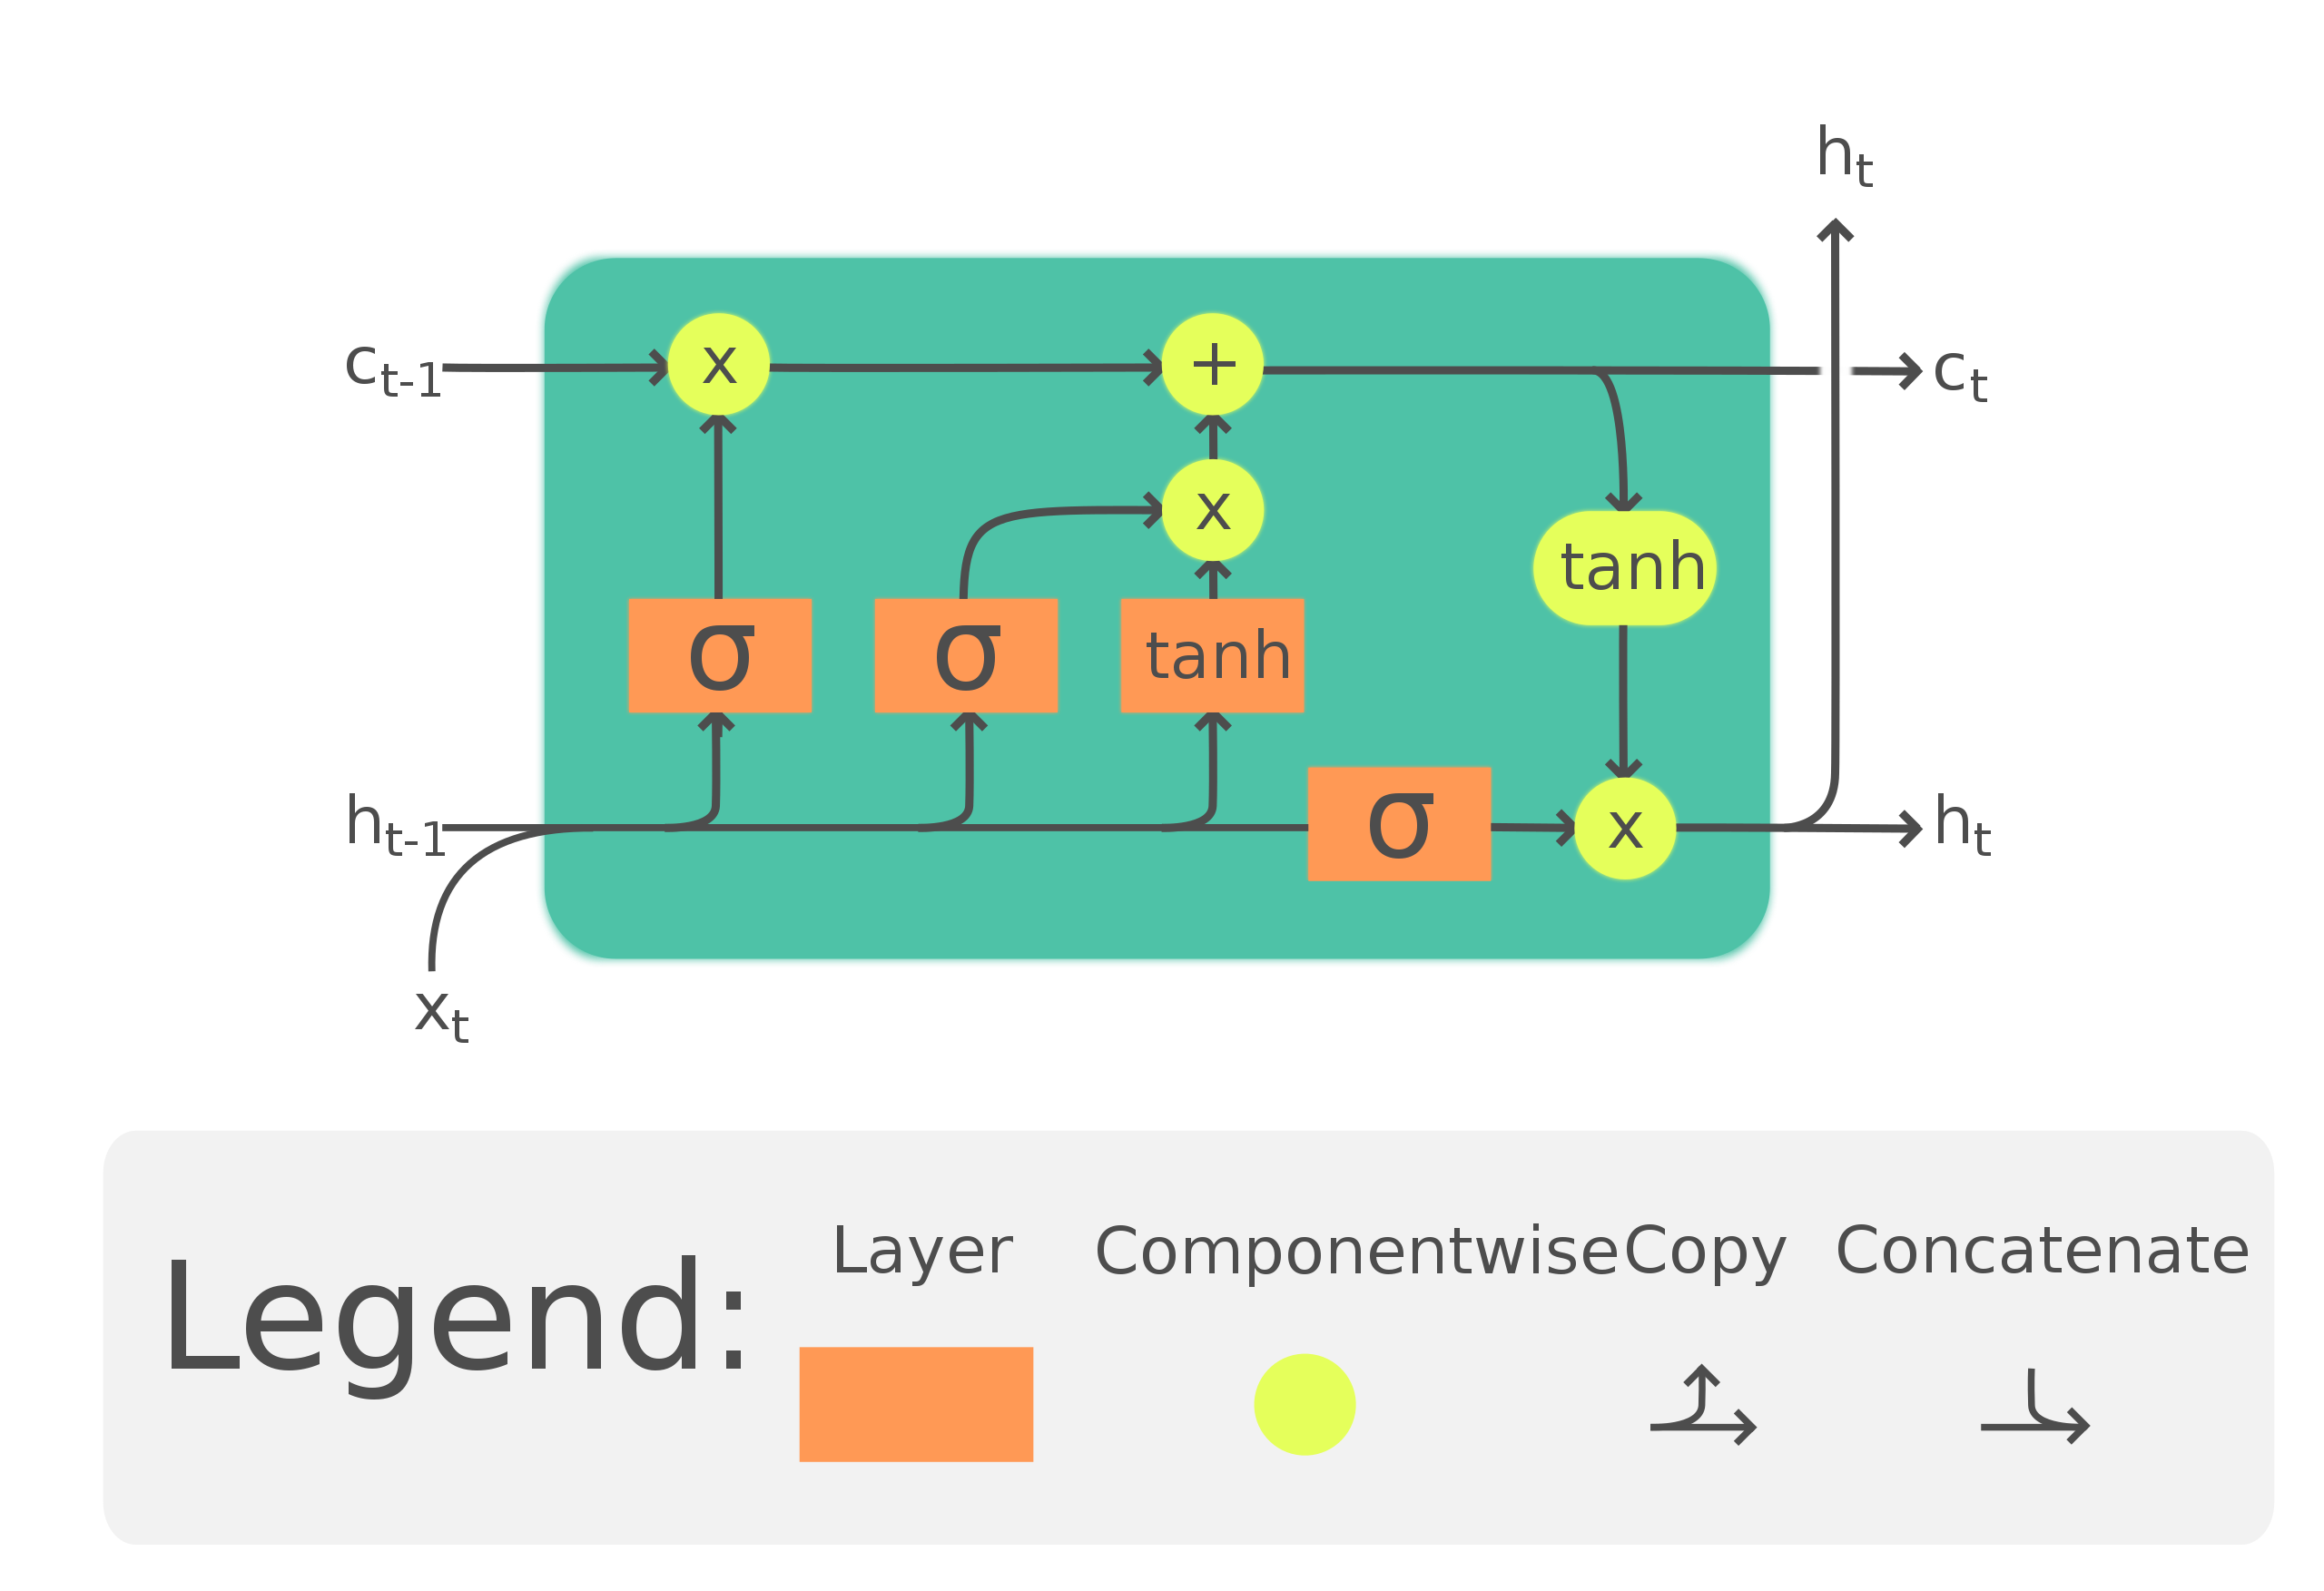
\includegraphics[width=0.8\textwidth]{lstm_cell.png}
      \end{minipage}
      \hfill
      \begin{minipage}[b]{0.45\textwidth}
        \textbf{LSTM}\par\medskip
          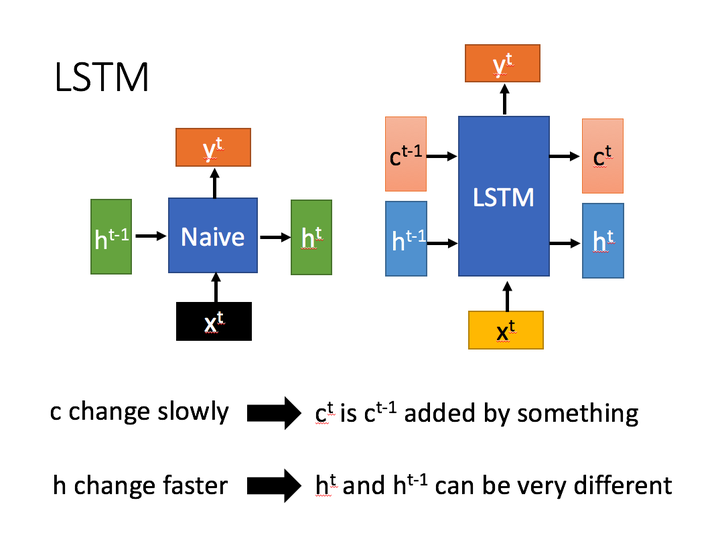
\includegraphics[width=0.8\textwidth]{lstm.jpg}
      \end{minipage}
    \end{figure}
  \end{itemize}
\end{frame}
\begin{frame}{Previous Work}
  \begin{itemize}
    \item Neural Machine Translation by Jointly Learning to Align and Translate (Bahdanau, 2014)
      \subitem{Landmark Paper}
      \subitem{Proposed New Architecture:}
          \subsubitem{bidirectional RNN as an encoder and an RNN decoder, with an attention mechanism in between}
      \subitem{Proposed initial idea of attention}
      \subitem{Model gave attention to particular hidden states when decoding each word}
      \subsubitem{Learned which words to give attention to during translation for each word of decoder}
      \subitem{Still required on RNN}
  \end{itemize}
\end{frame}

\begin{frame}{Context}
 \begin{itemize}
    \item What issue are they solving?
       \subitem{Previous Work: RNN, LSTM, GRU}
       \subitem{Slow to train (inefficient / not parallelizable)}
       \subsubitem{factorization tricks help efficiency but still slow}
       \subitem{Suffer from exploding or vanishing gradients}
       \subitem{Cannot handle very long-term dependencies}
       \subsubitem{In Seq-Seq models, decoder only accesses last hidden state. Early information in sentence can be lost.}
  \end{itemize}
\end{frame}

\begin{frame}{Scaled Dot Product Attention}
  \begin{itemize}
    \item Key algorithm in transformers
    \item  $ \displaystyle {\text{Attention}}(Q,K,V)={\text{softmax}}\left({\frac {QK^{T}}{\sqrt {d_{k}}}}\right)V $
    \item ${\displaystyle Q,K,V}$ are the query, key, and value matrices, $d_{k}$ is the dimension of the keys.  Dividing by $\sqrt {d_{k}}$ makes algorithm easier to train
    \item Attention weights: how likely each query matches key (used for weighted sum of values)
    \item NOT stepping through a sequence like with a RNN
  \end{itemize}
\end{frame}

\begin{frame}{Scaled Dot Product Attention}
The example below shows how correlations are identified once a network has been trained and has the right weights. When looking at the word "that" in the sentence "see that girl run", the network should be able to identify "girl" as a highly correlated word. For simplicity this example focuses on the word "that".
    \begin{figure}
      \centering
      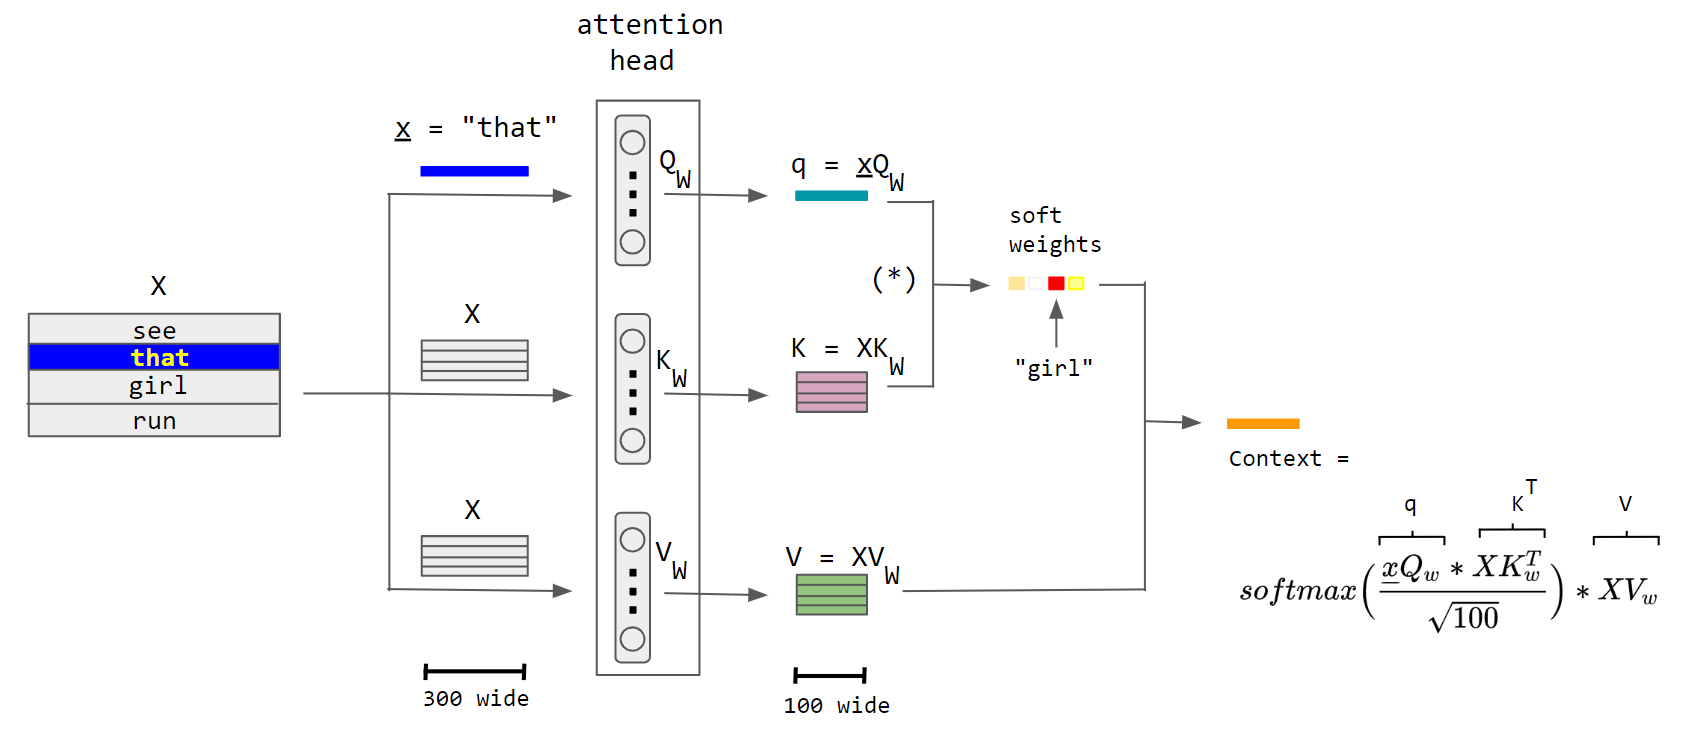
\includegraphics[width=1\textwidth]{Attention-qkv.png}
    \end{figure}
\end{frame}

\begin{frame}{Multi-Head Attention}
  \begin{itemize}
    \item
    ${\displaystyle {\text{MultiHead}}(Q,K,V)={\text{Concat}}({\text{head}}_{1},...,{\text{head}}_{h})W^{O}}$
    ${\displaystyle {\text{head}}_{i}={\text{Attention}}(QW_{i}^{Q},KW_{i}^{K},VW_{i}^{V})}$
\\  ${\displaystyle W_{i}^{Q},W_{i}^{K},W_{i}^{V}}$, and
    ${\displaystyle W^{O}}$ are parameter matrices.
    \begin{figure}
      \centering
      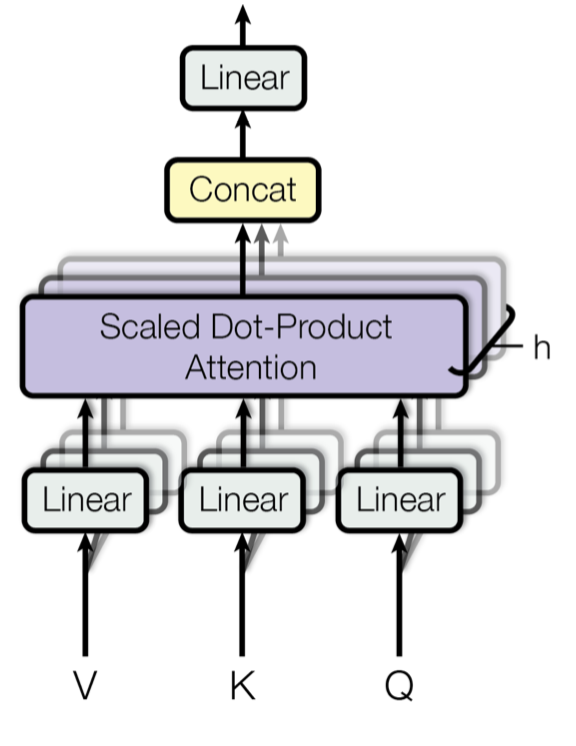
\includegraphics[width=0.3\textwidth]{multi-head-attention.png}
    \end{figure}
    \item Allows for model to focus on different positions
    \item Gives attention layer multiple “representation subspaces”
    \item No longer need to oversaturate one attention mechanism
  \end{itemize}
\end{frame}

\begin{frame}{Positional Encoding}
  \begin{itemize}
    \item Need for information about the position and order of tokens in a sequence
    \item Positional Embedding: Vector that represents position of each token
  \end{itemize}
\end{frame}

\begin{frame}{Transformer}
  \begin{tabular}{cl}  
    \begin{tabular}{c}
      \parbox{0.4\linewidth}{
        \begin{itemize}
          \fontsize{8}{8}\selectfont\setlength\itemindent{0pt}
          \item Tokenizers, which convert text into tokens.
          \item A single embedding layer, which converts tokens and positions of the tokens into vector representations.
          \item Transformer layers, which carry out repeated transformations on the vector representations, extracting more and more linguistic information. These consist of alternating attention and feedforward layers.
          \item (optional) Un-embedding layer
        \end{itemize}
      }
    \end{tabular}
    &
    \begin{tabular}{l}
      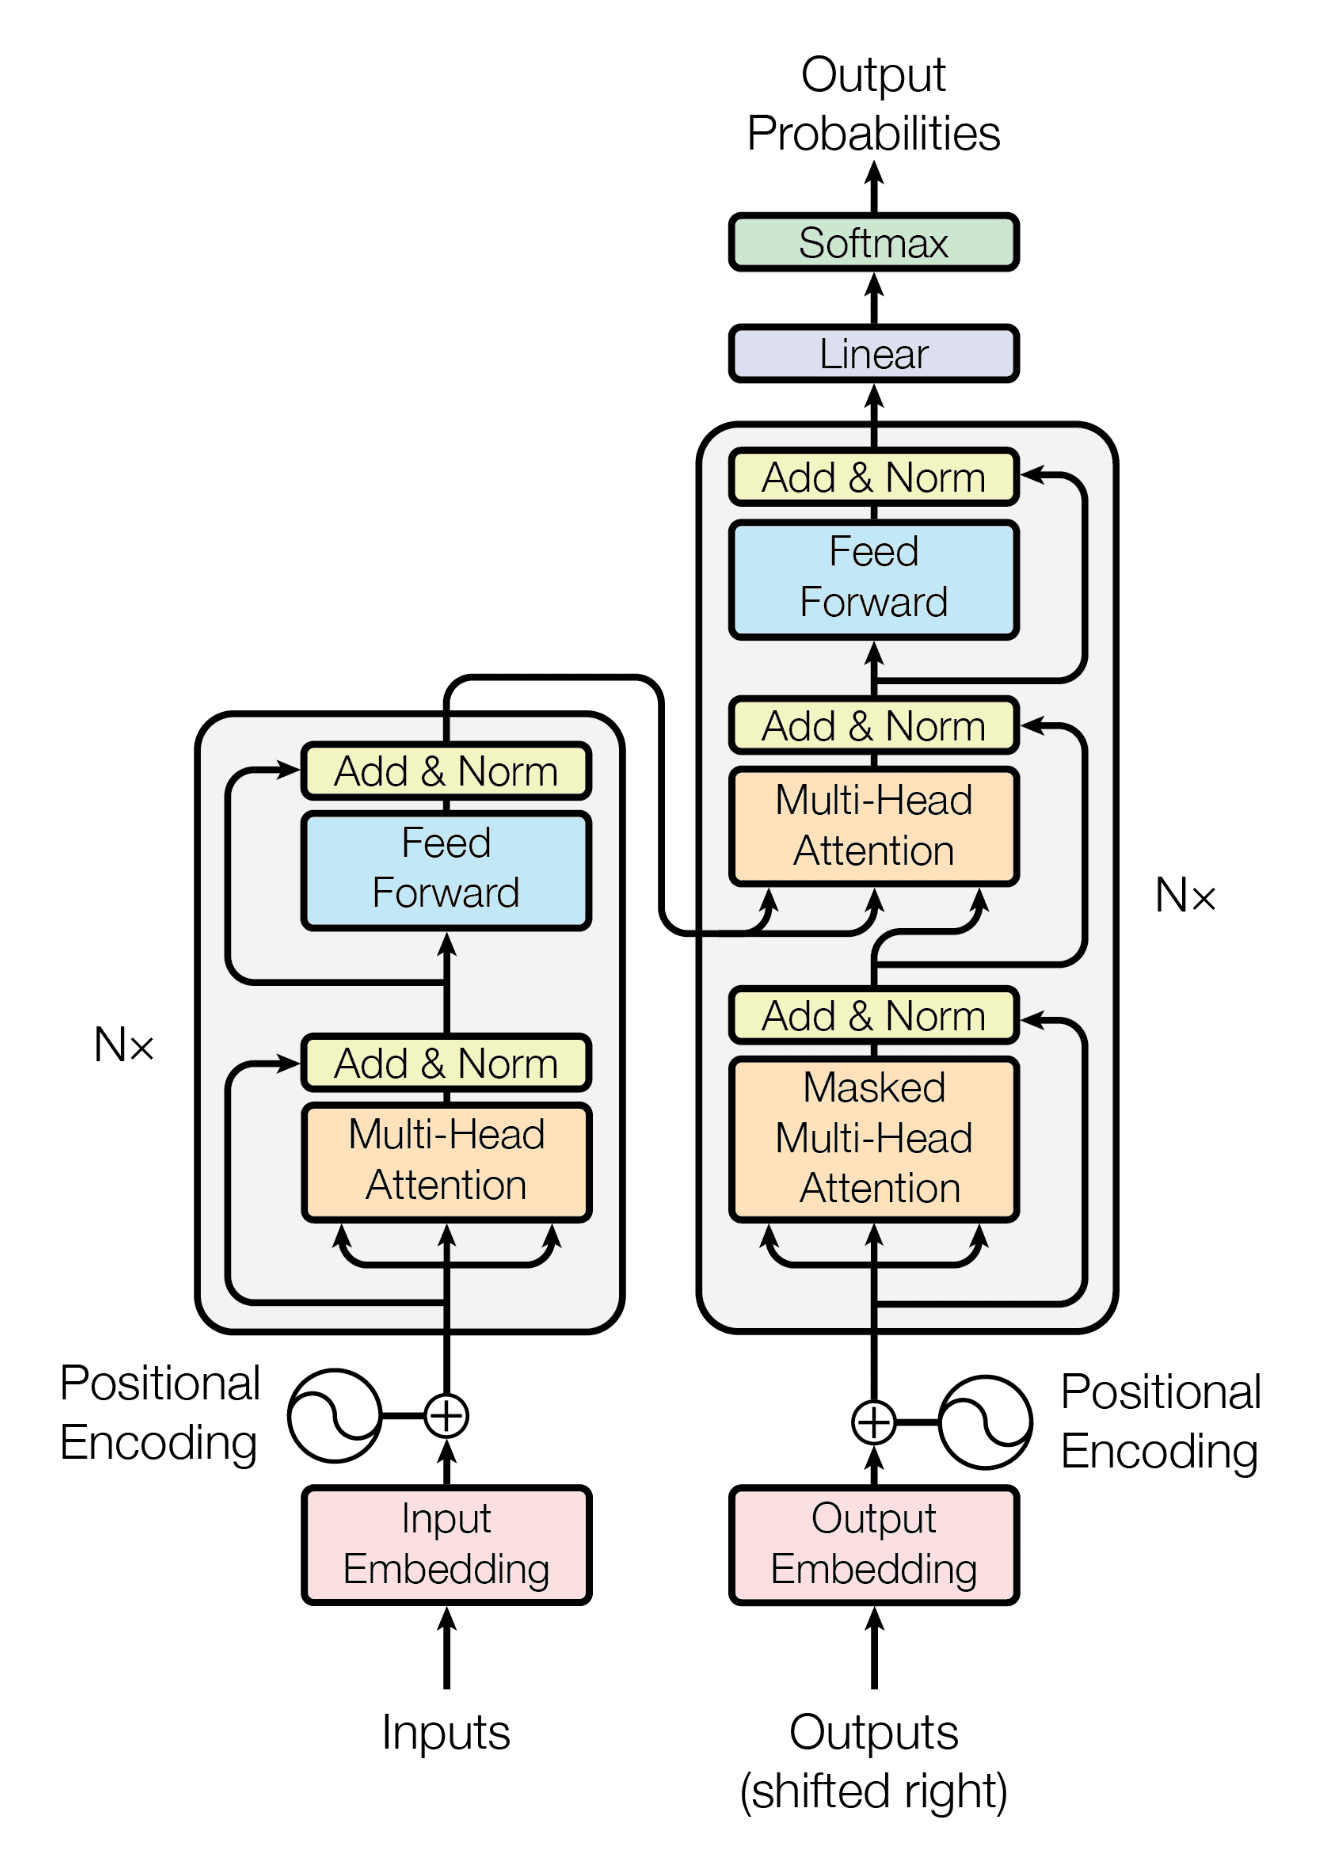
\includegraphics[width=0.5\textwidth]{transformer.png}
    \end{tabular}  \\
  \end{tabular}
\end{frame}

\begin{frame}{A language translation example}
\begin{figure}
  \begin{minipage}[b]{0.4\textwidth}
    \par\medskip
    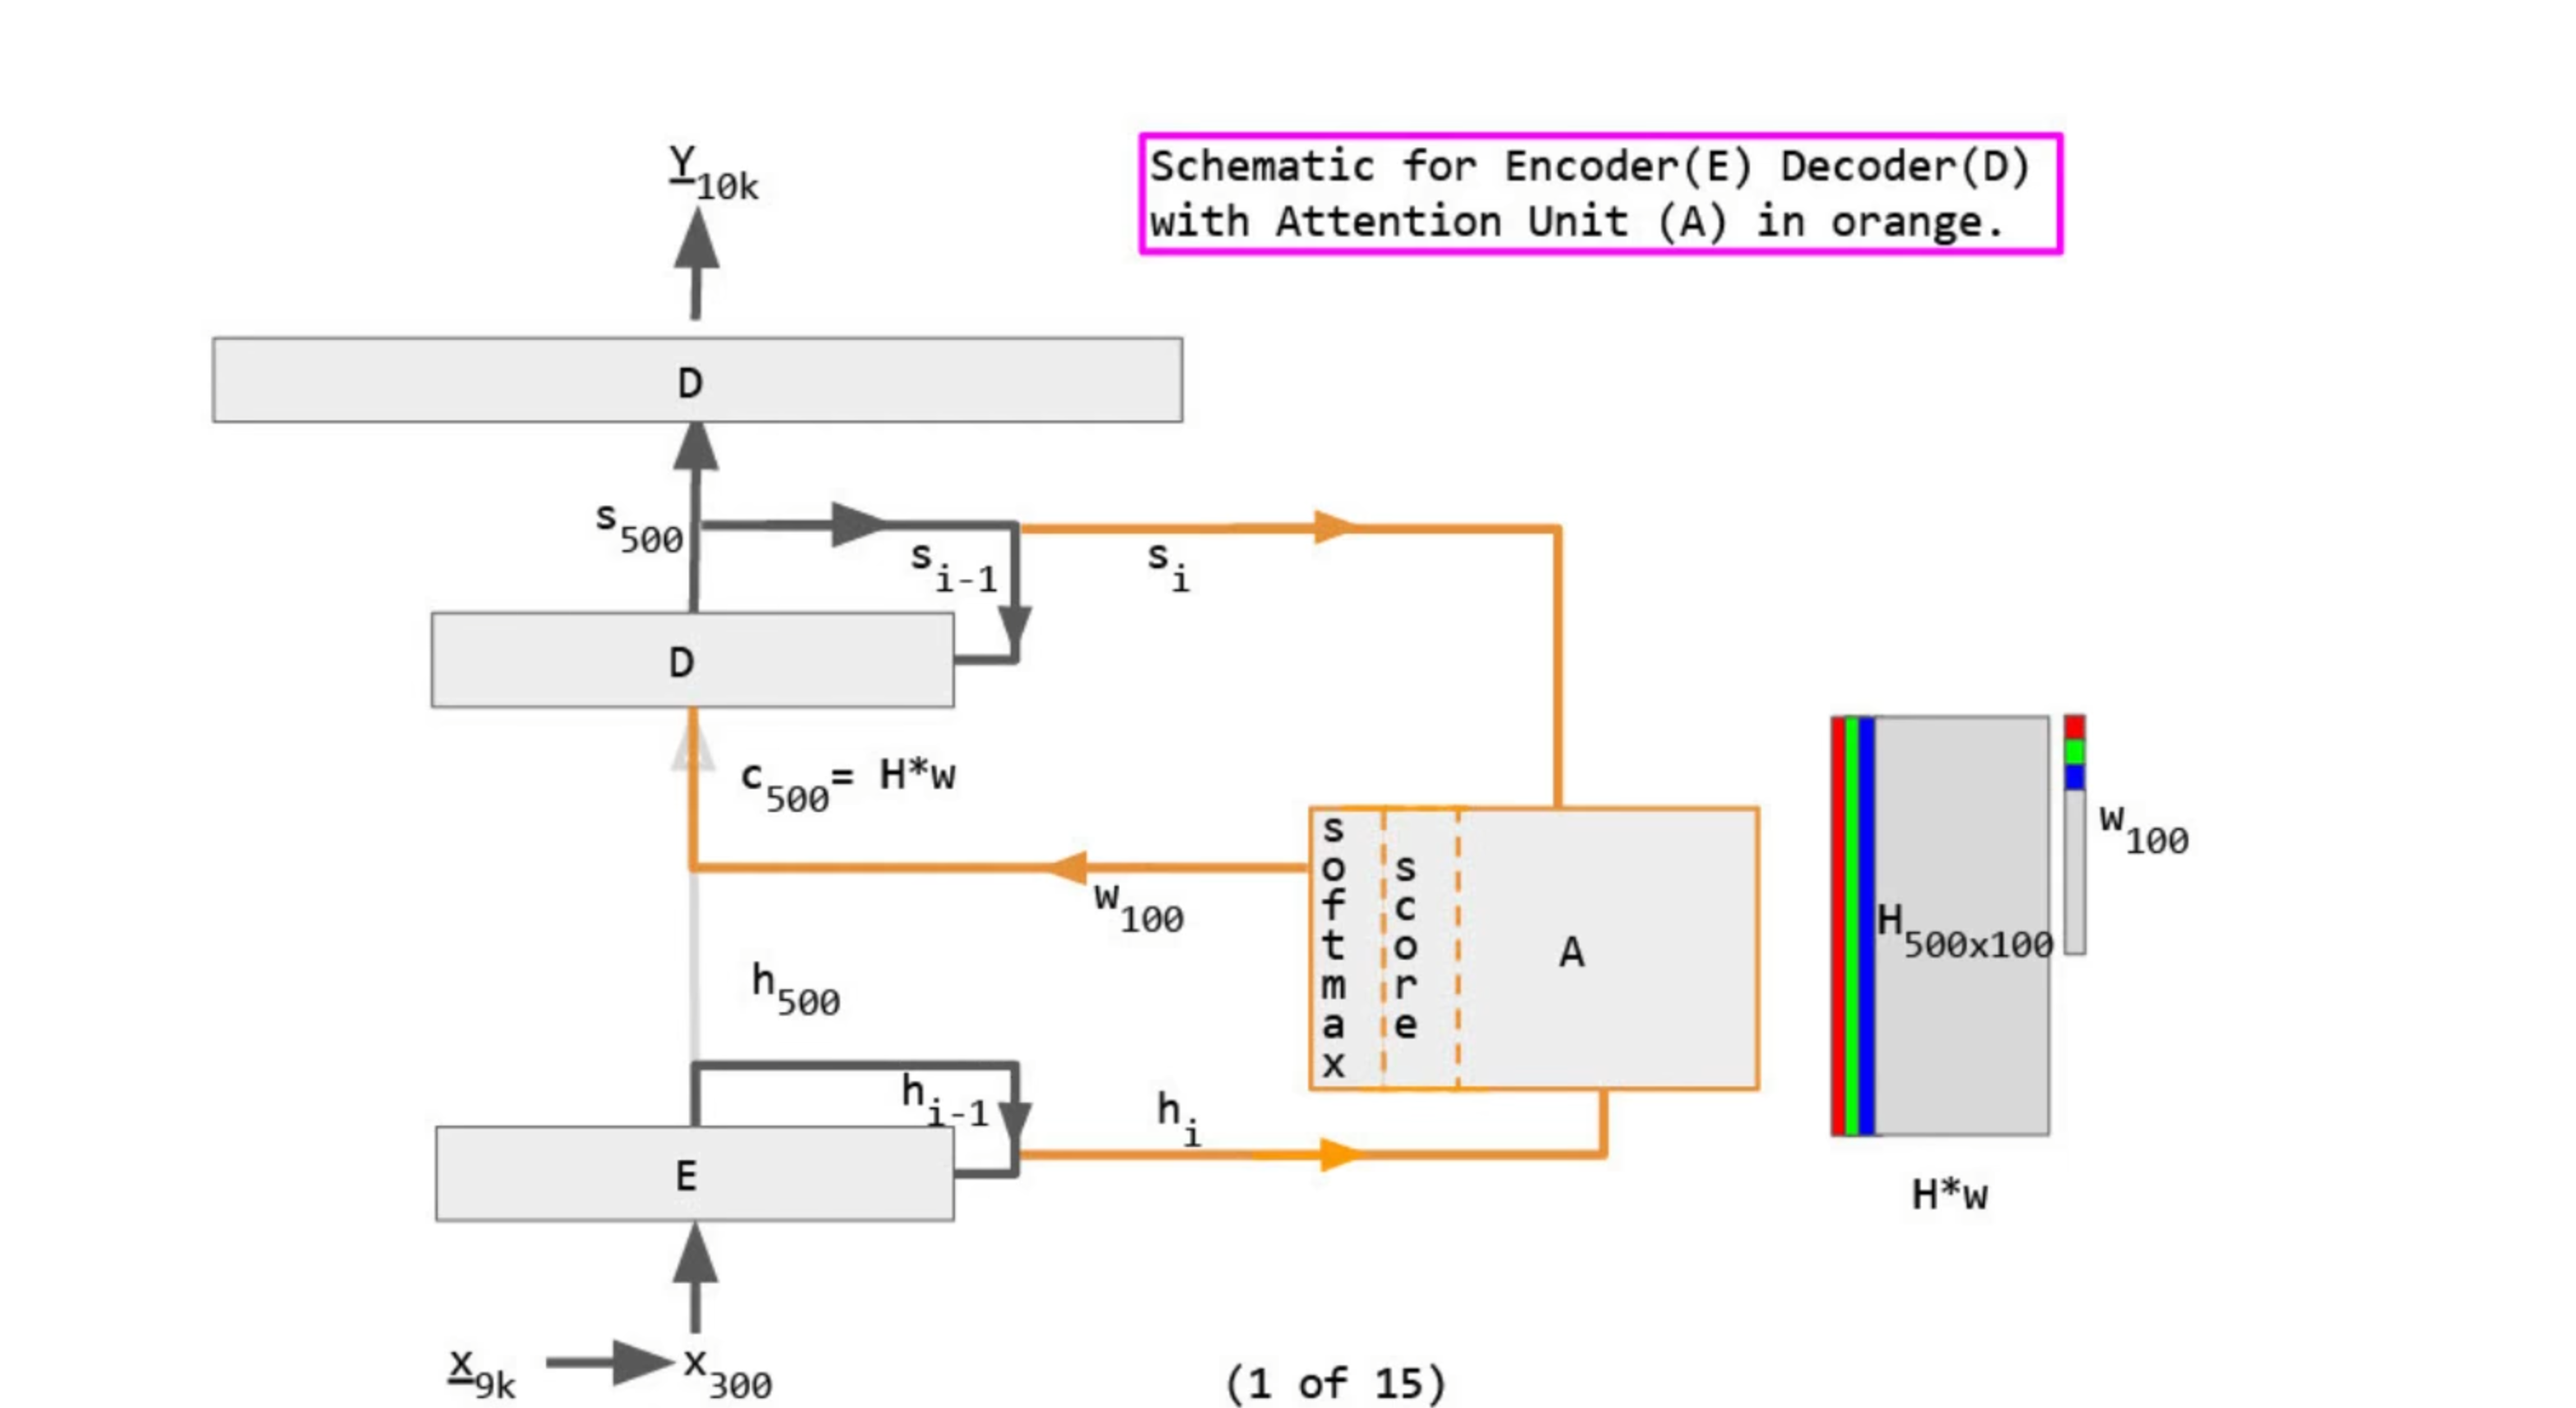
\includegraphics[width=1.3\textwidth]{./translation/1.png}
  \end{minipage}
  \hfill
  \begin{minipage}[b]{0.4\textwidth}
    \par\medskip
    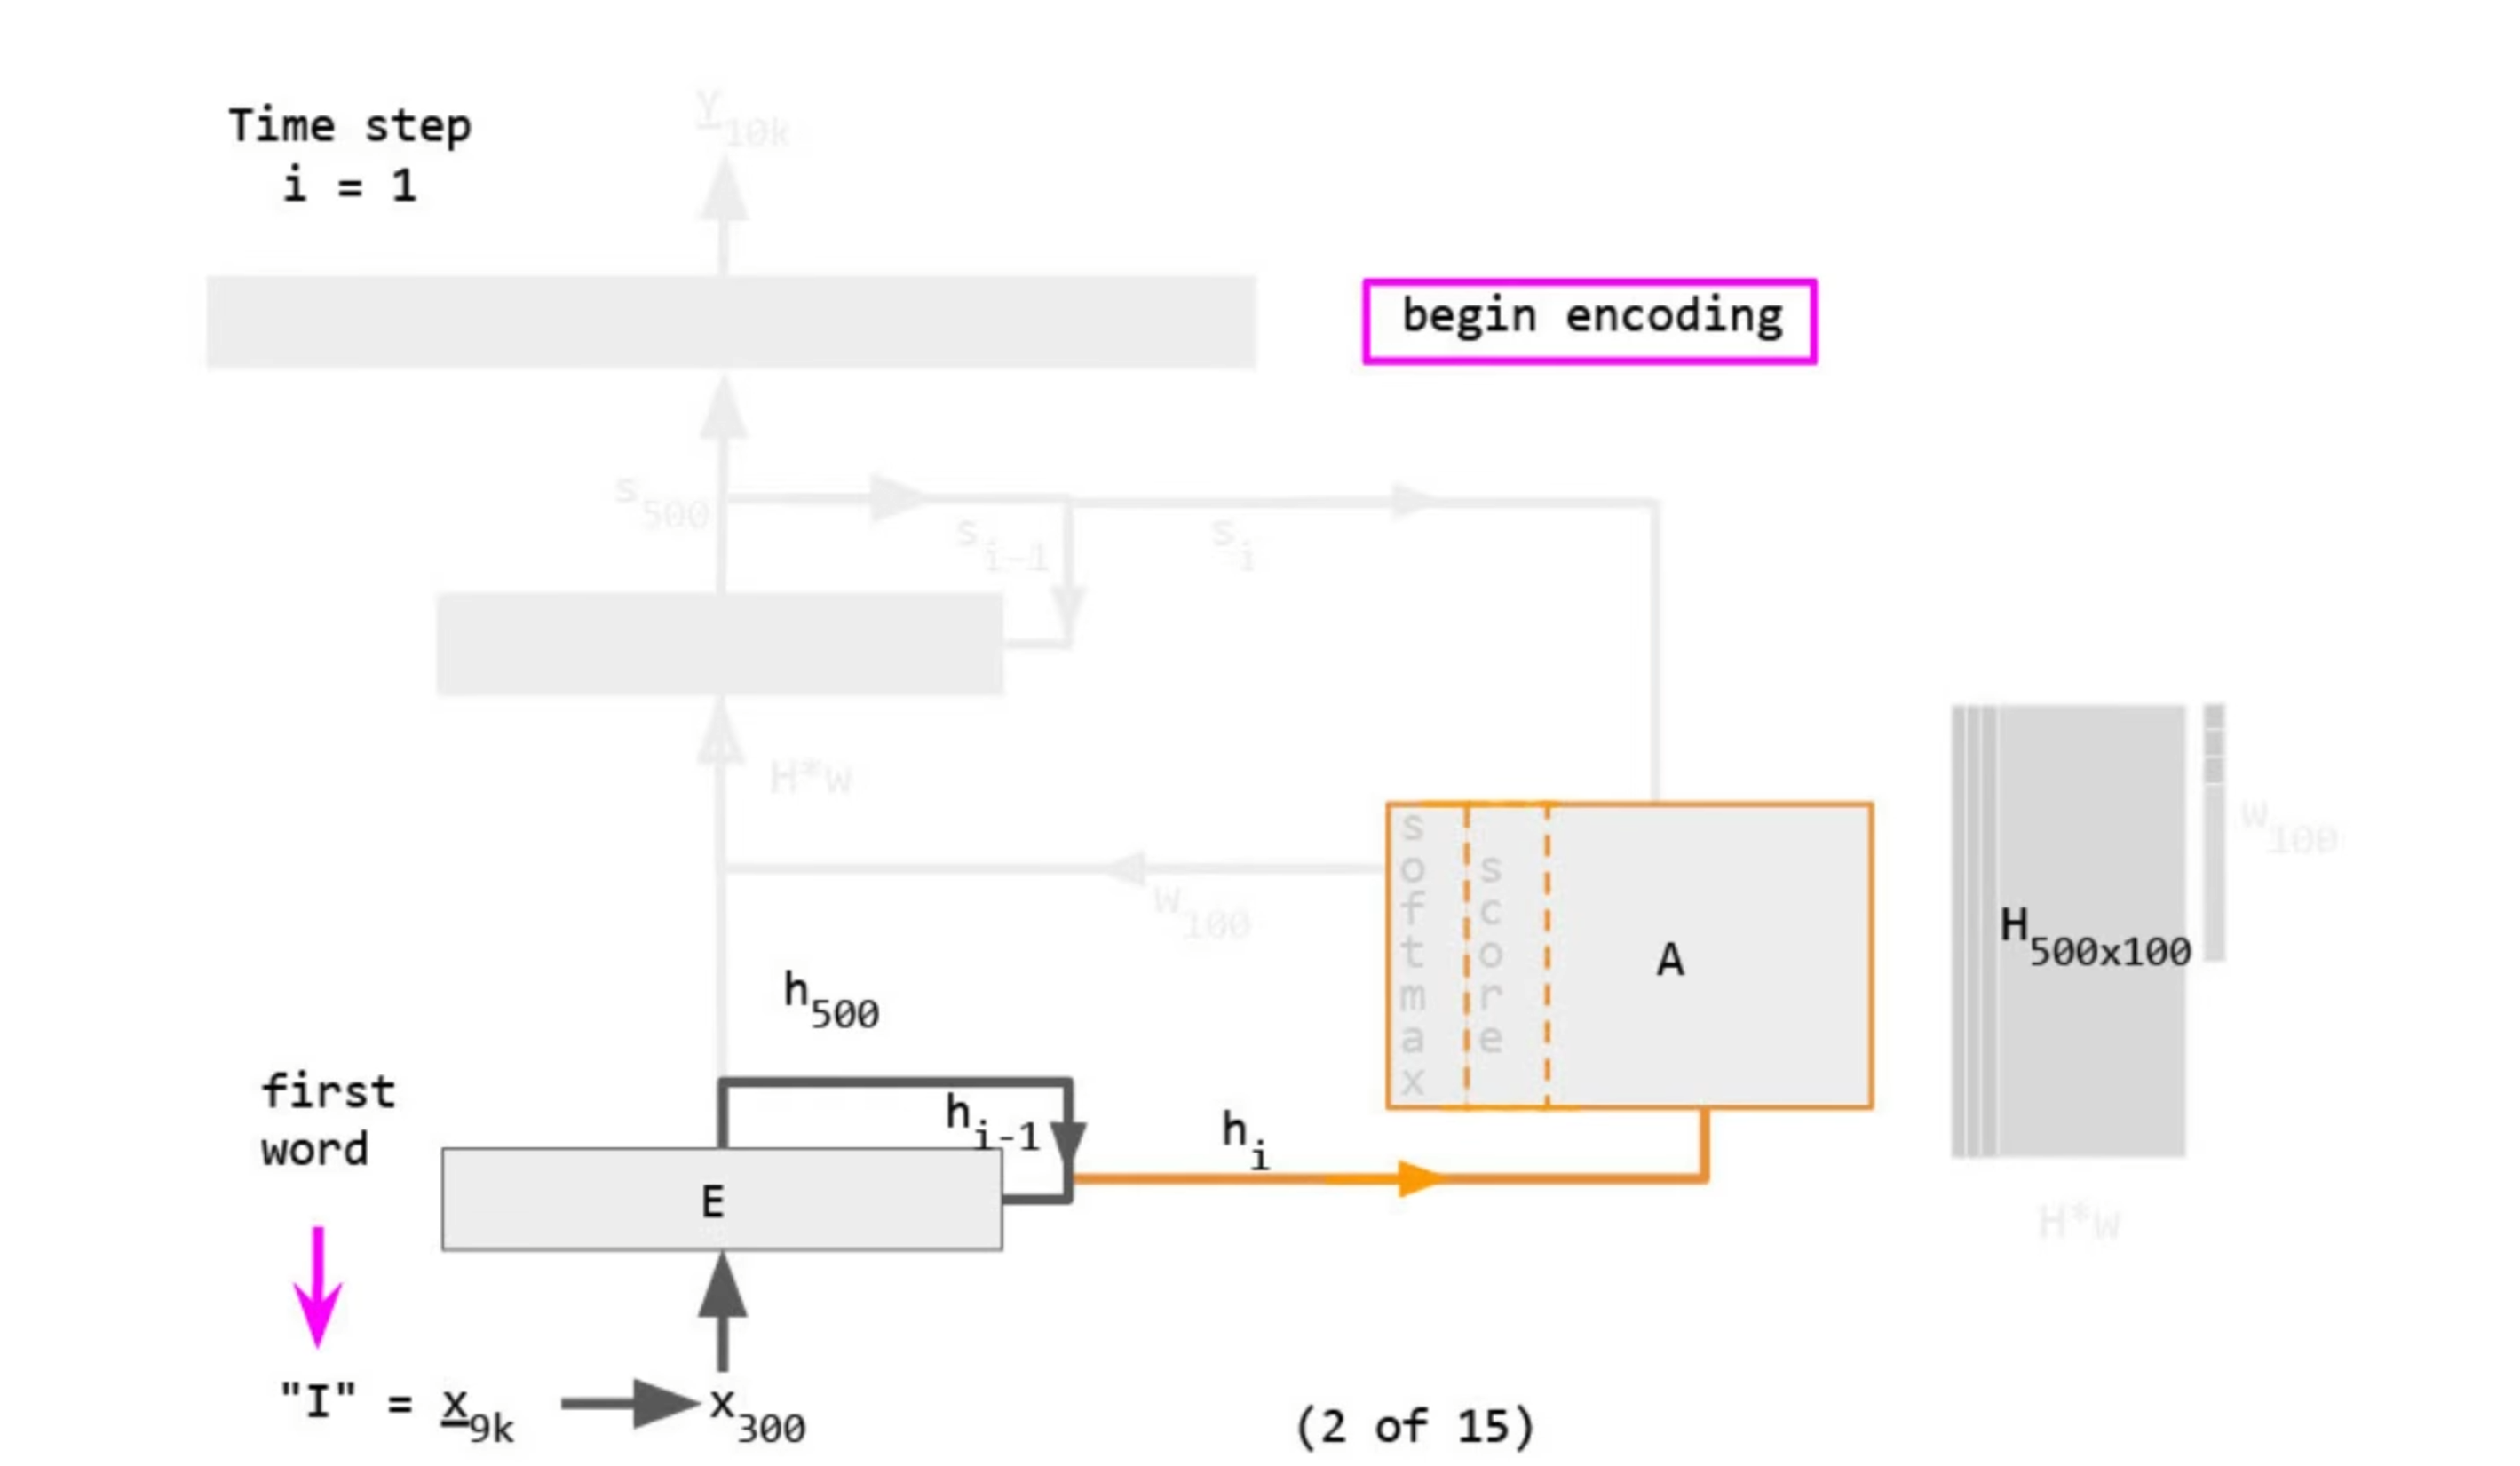
\includegraphics[width=1.3\textwidth]{./translation/2.jpg}
  \end{minipage}
  \begin{minipage}[b]{0.4\textwidth}
    \par\medskip
    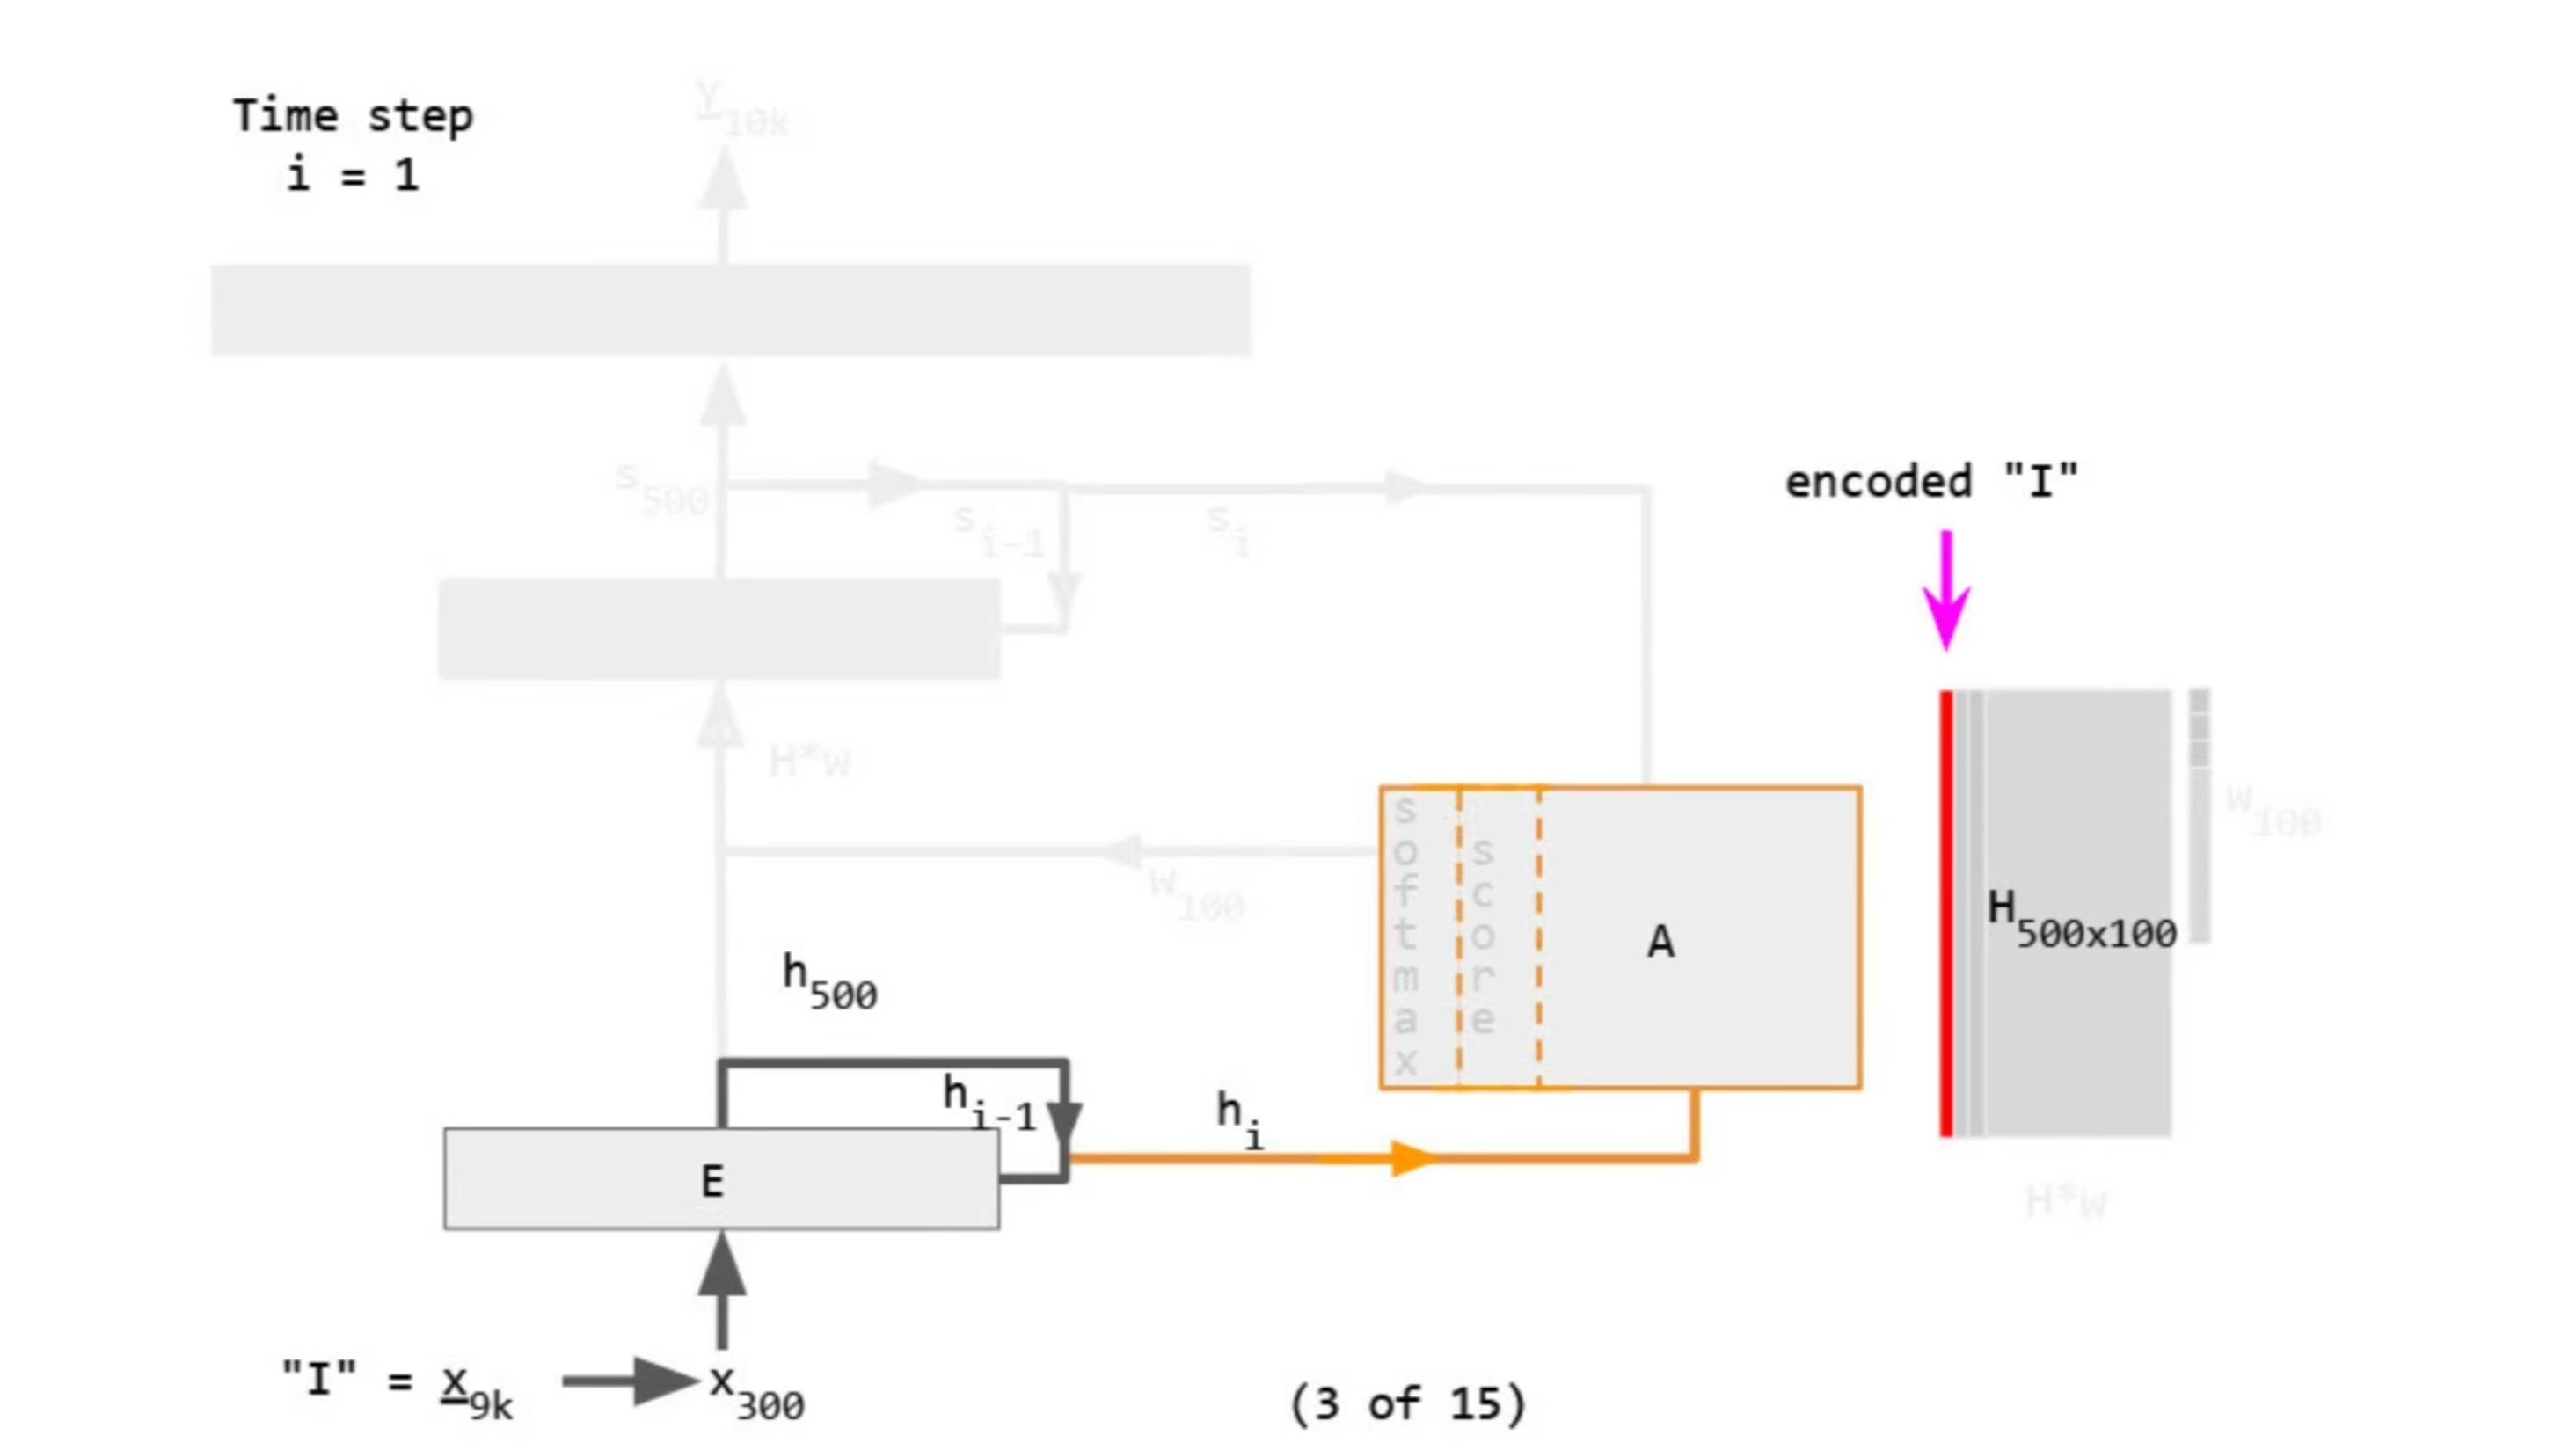
\includegraphics[width=1.3\textwidth]{./translation/3.jpg}
  \end{minipage}
\end{figure}
\end{frame}

\begin{frame}{A language translation example}
\begin{figure}
  \begin{minipage}[b]{0.4\textwidth}
    \par\medskip
    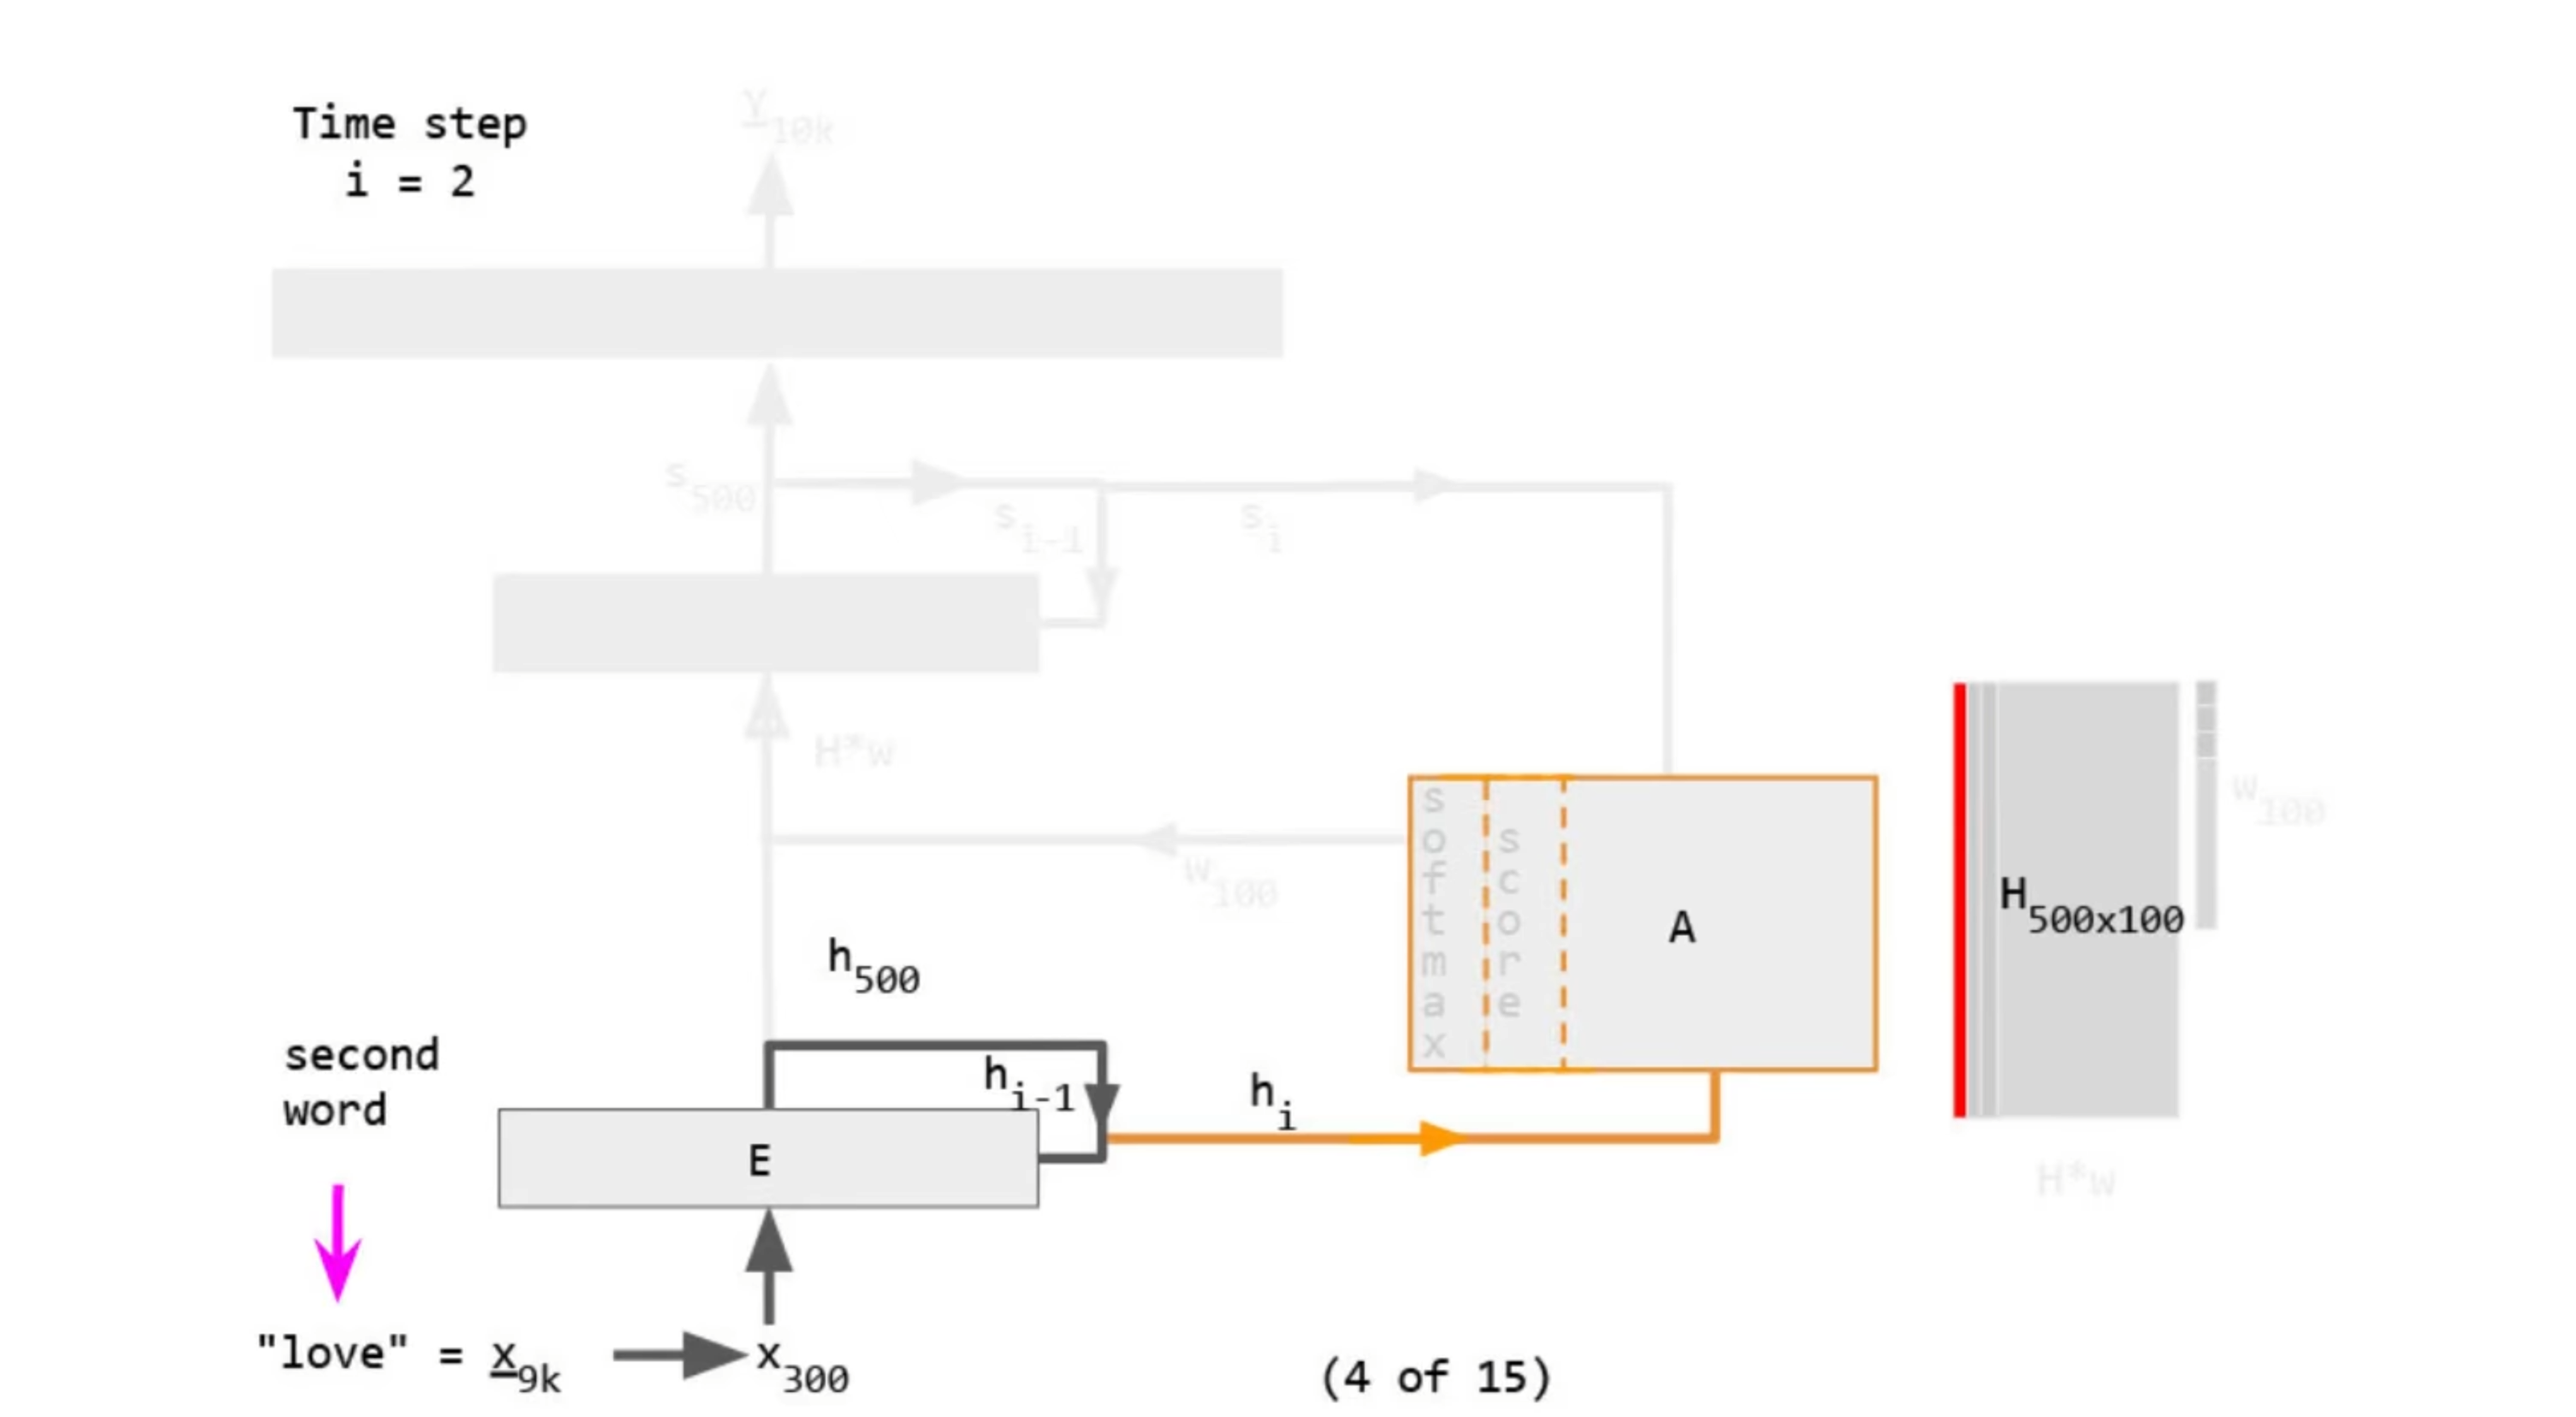
\includegraphics[width=1.3\textwidth]{./translation/4.jpg}
  \end{minipage}
  \hfill
  \begin{minipage}[b]{0.4\textwidth}
    \par\medskip
    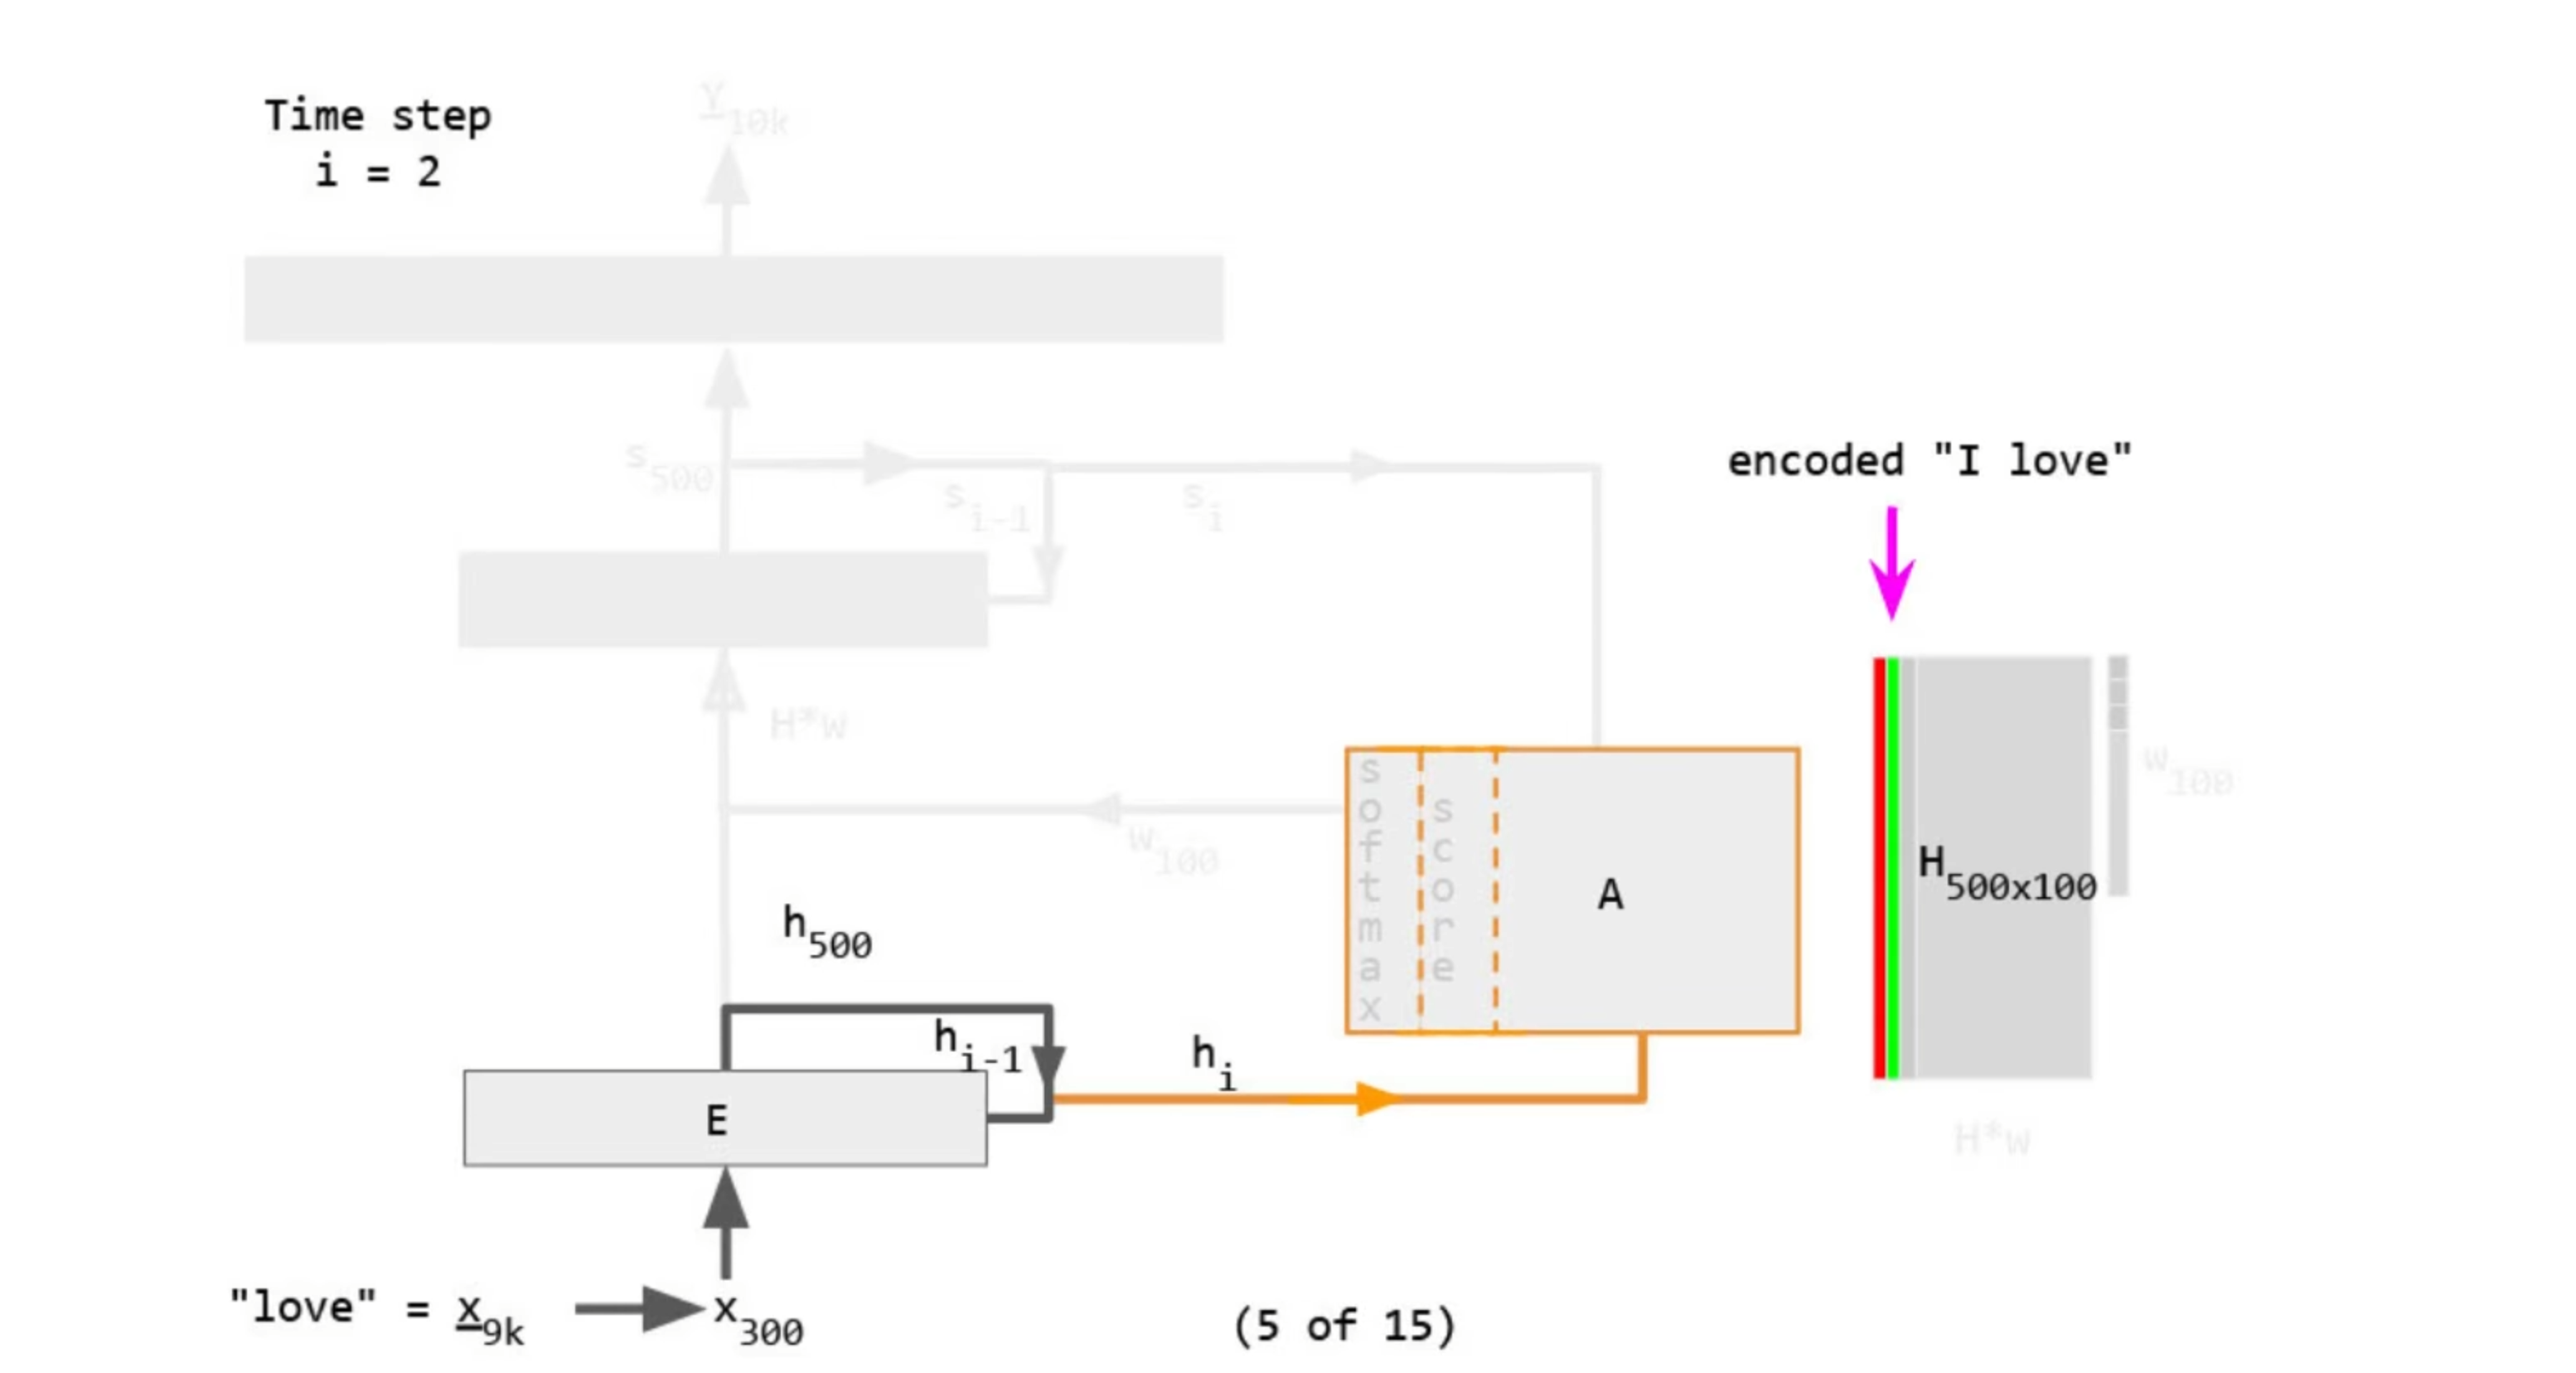
\includegraphics[width=1.3\textwidth]{./translation/5.jpg}
  \end{minipage}
  \begin{minipage}[b]{0.4\textwidth}
    \par\medskip
    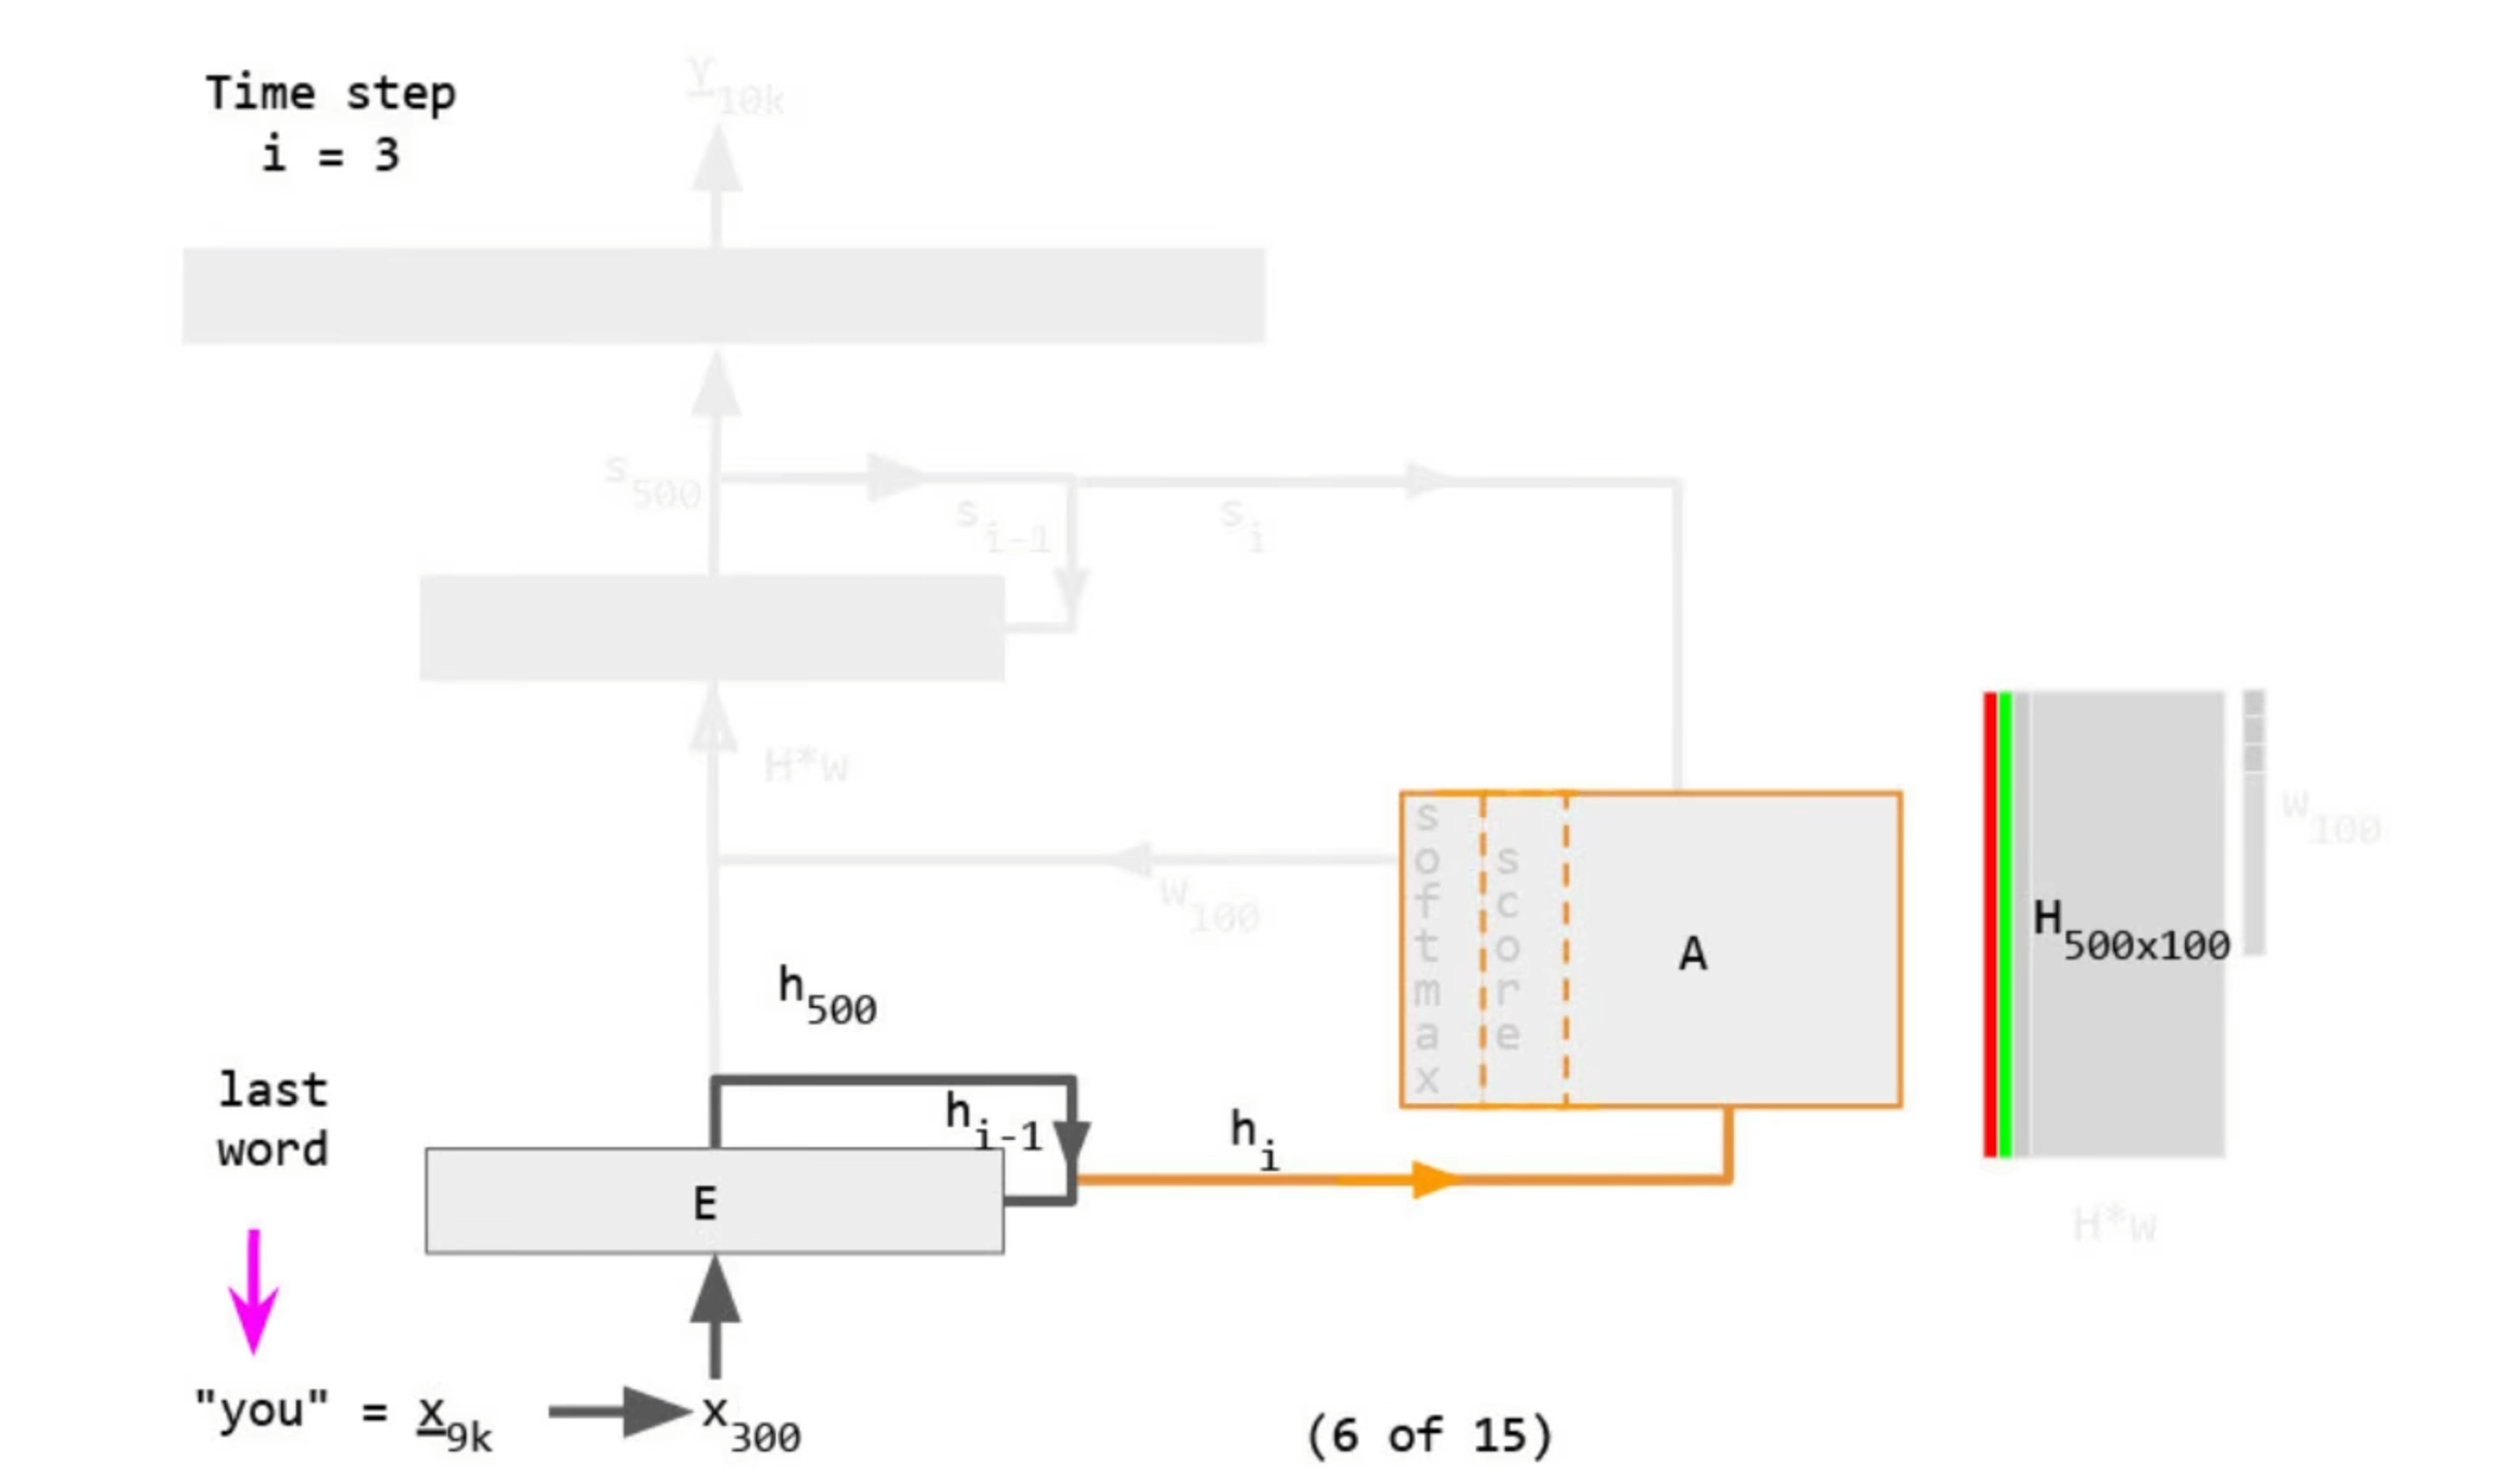
\includegraphics[width=1.3\textwidth]{./translation/6.jpg}
  \end{minipage}
\end{figure}
\end{frame}

\begin{frame}{A language translation example}
\begin{figure}
  \begin{minipage}[b]{0.4\textwidth}
    \par\medskip
    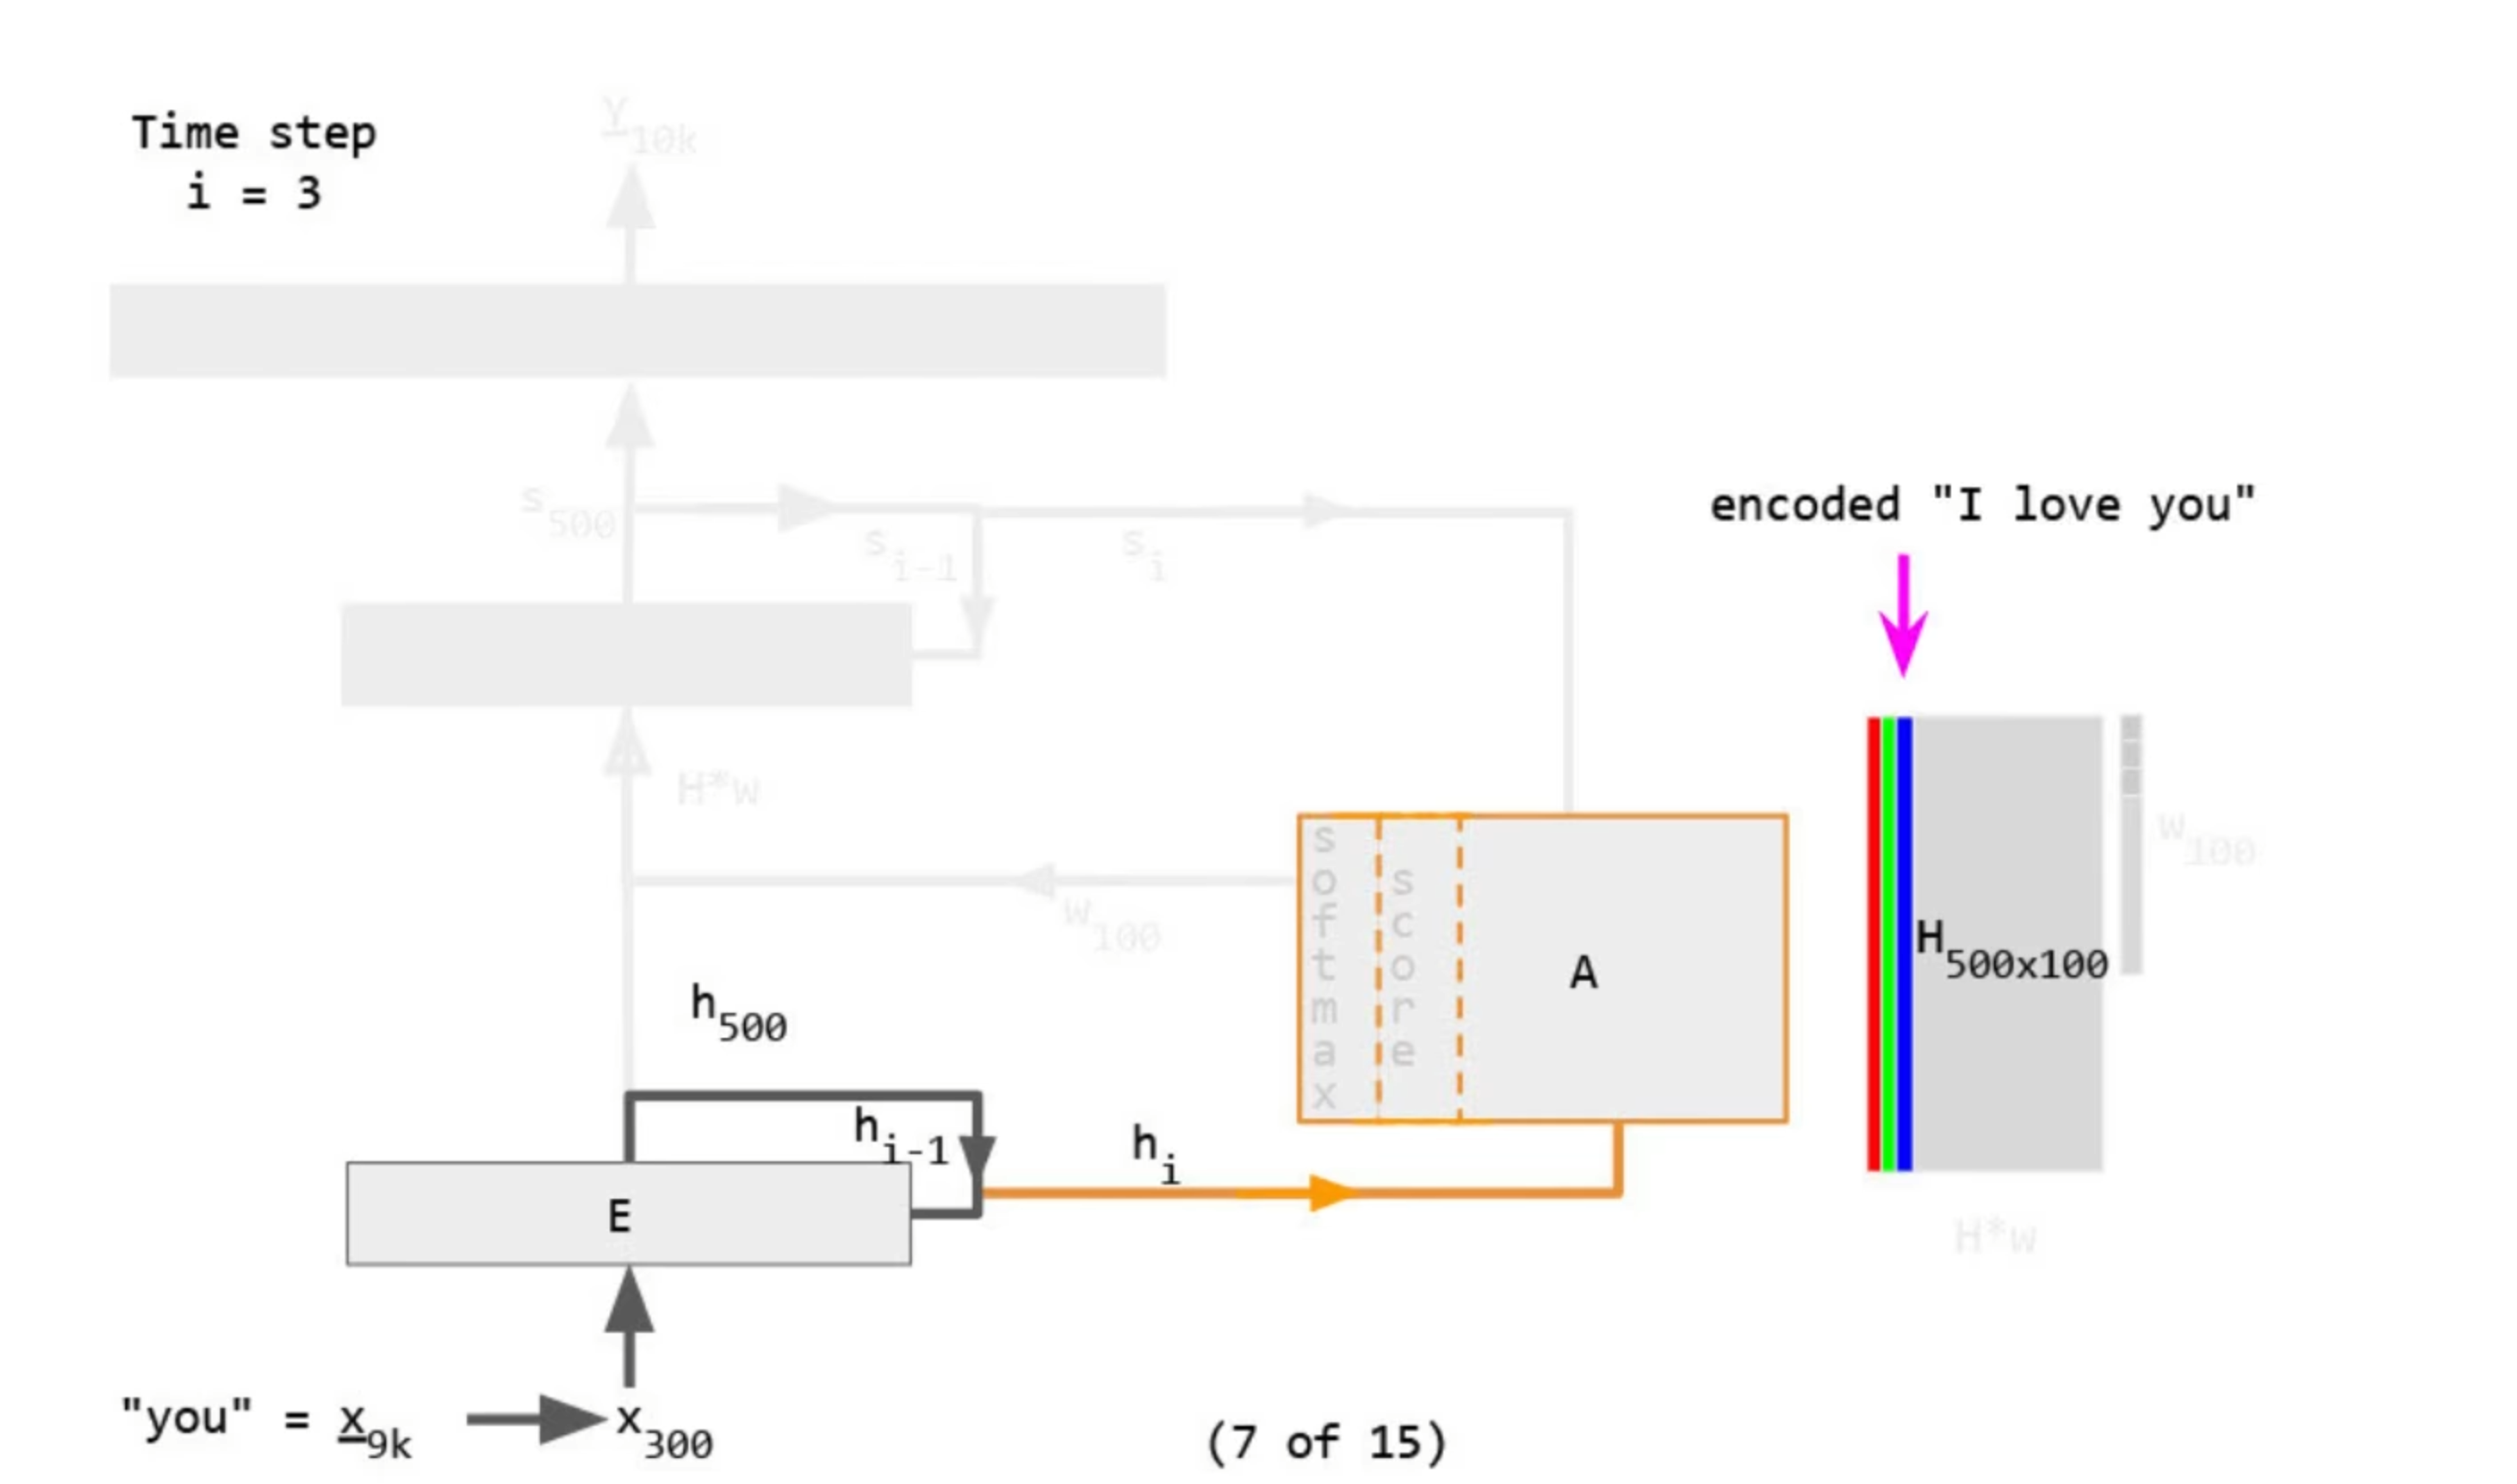
\includegraphics[width=1.3\textwidth]{./translation/7.jpg}
  \end{minipage}
  \hfill
  \begin{minipage}[b]{0.4\textwidth}
    \par\medskip
    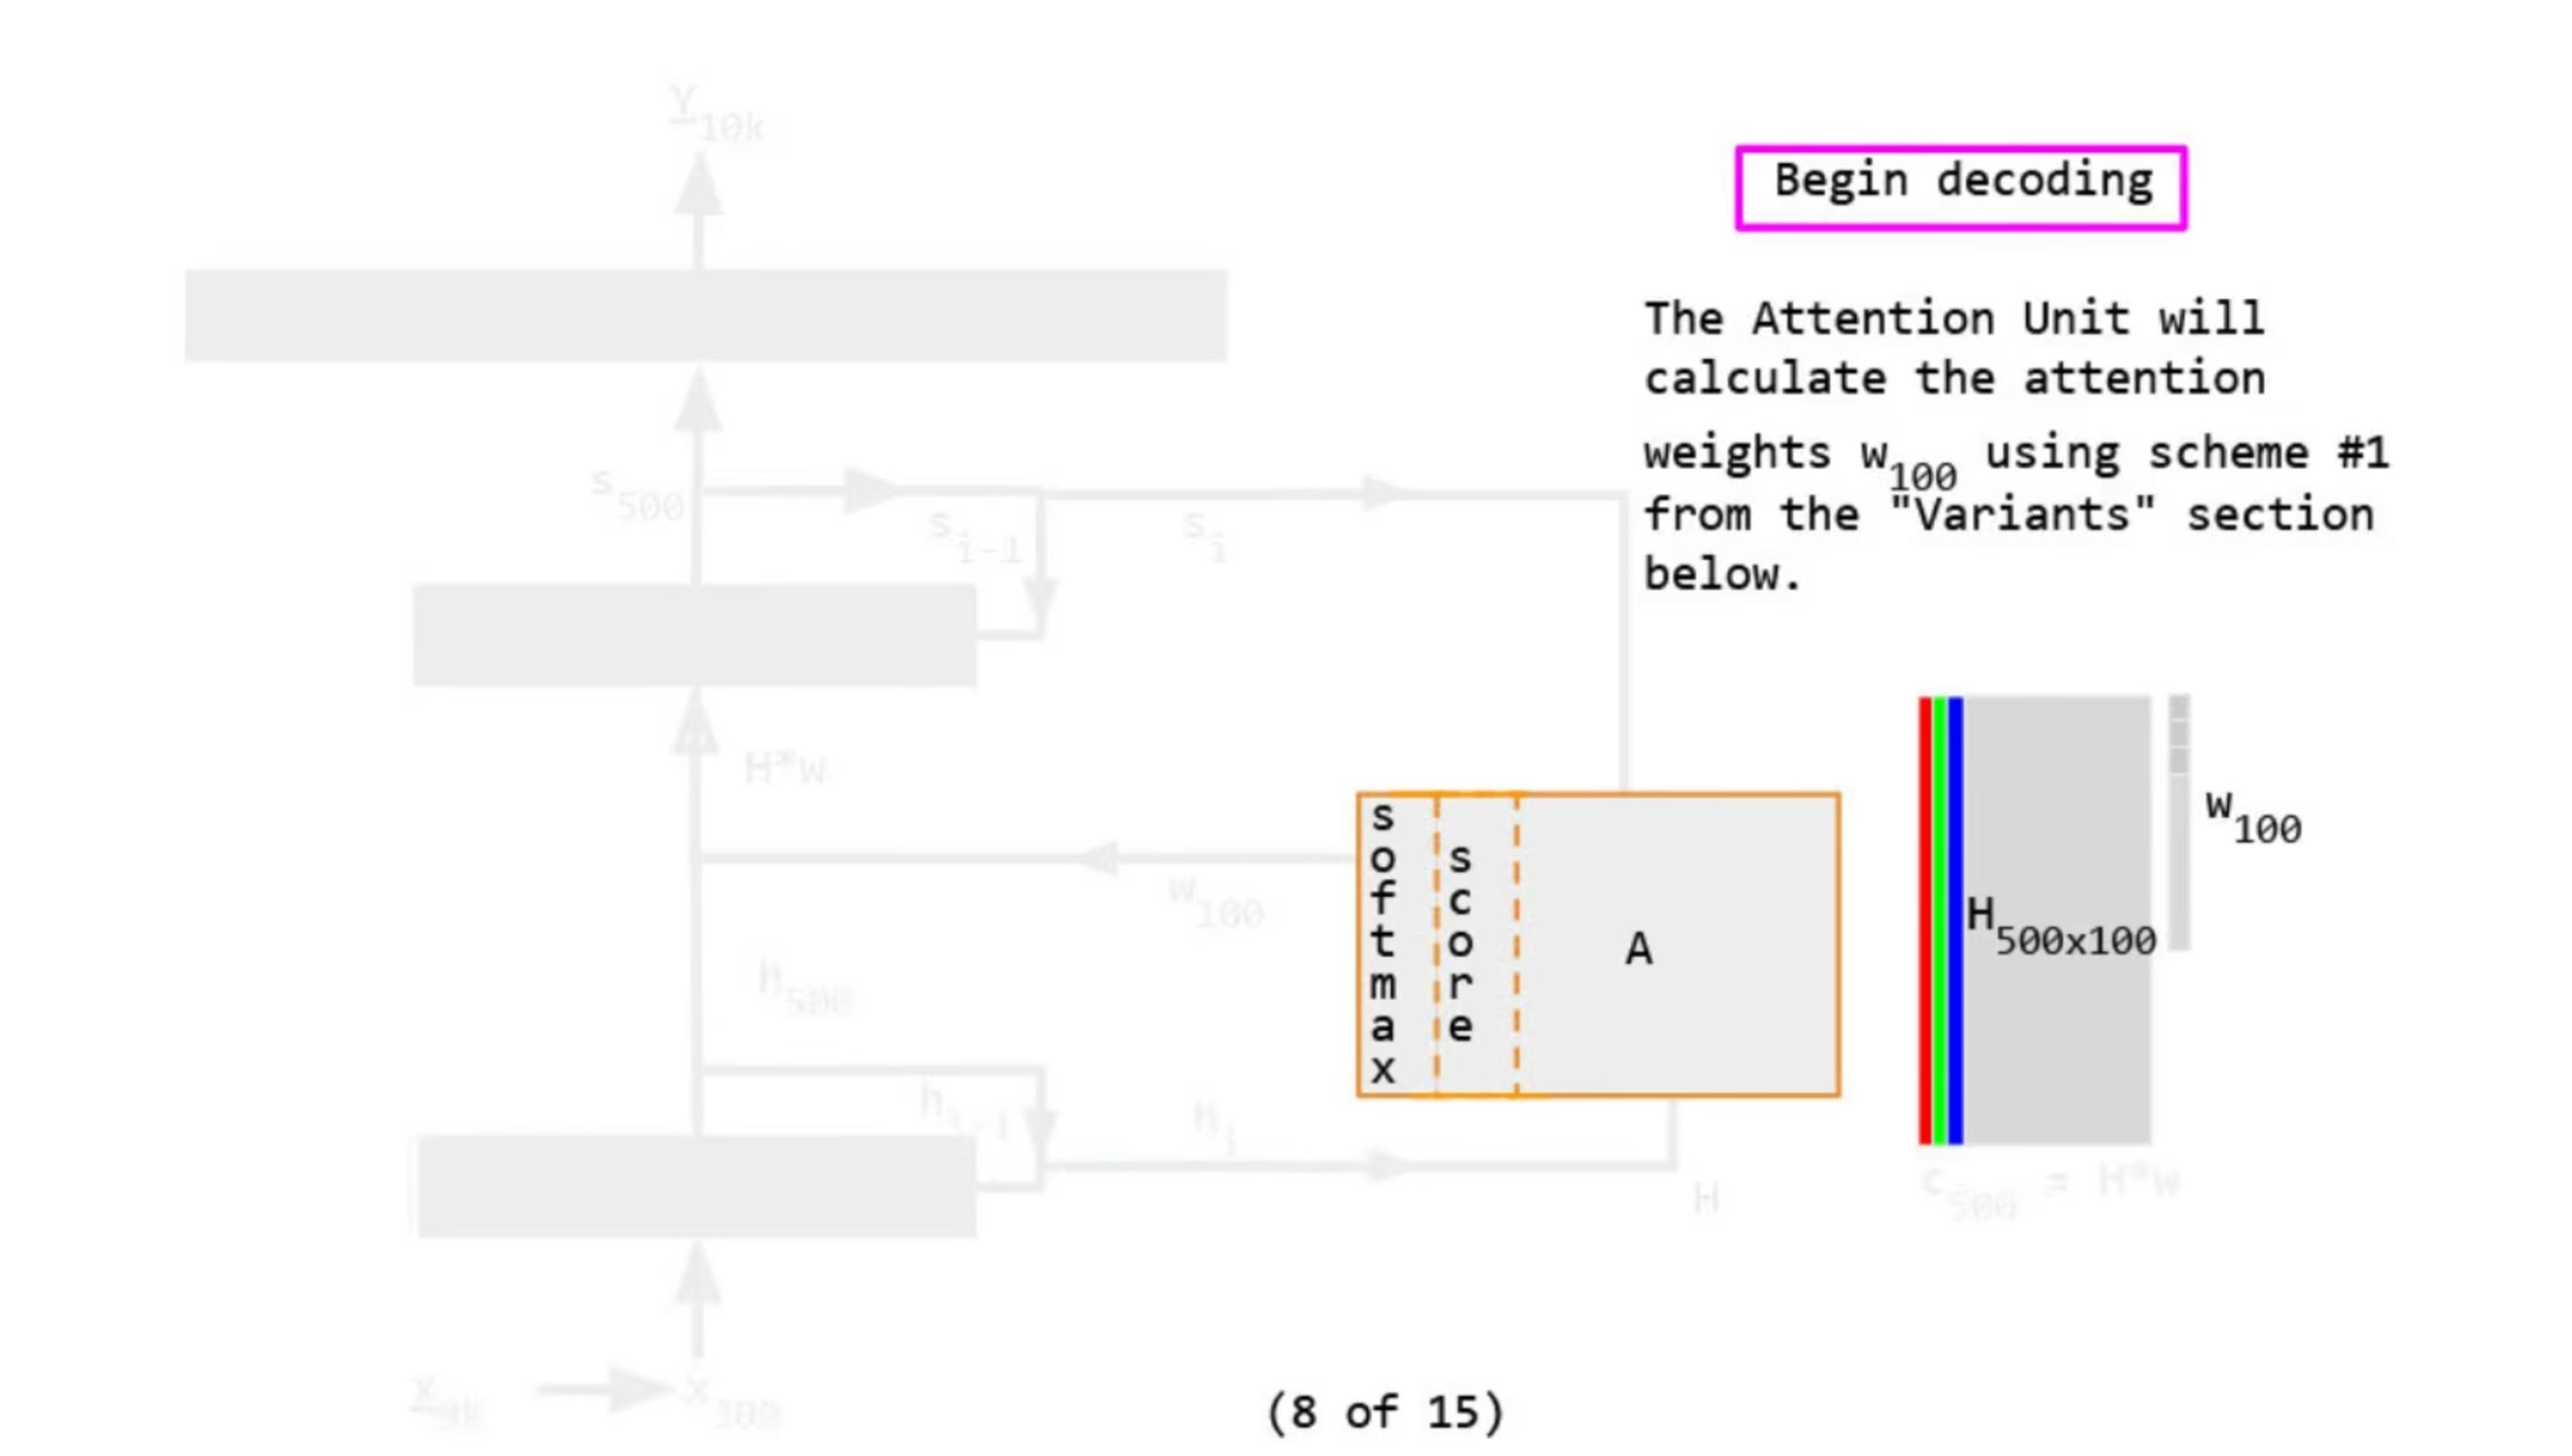
\includegraphics[width=1.3\textwidth]{./translation/8.jpg}
  \end{minipage}
  \begin{minipage}[b]{0.4\textwidth}
    \par\medskip
    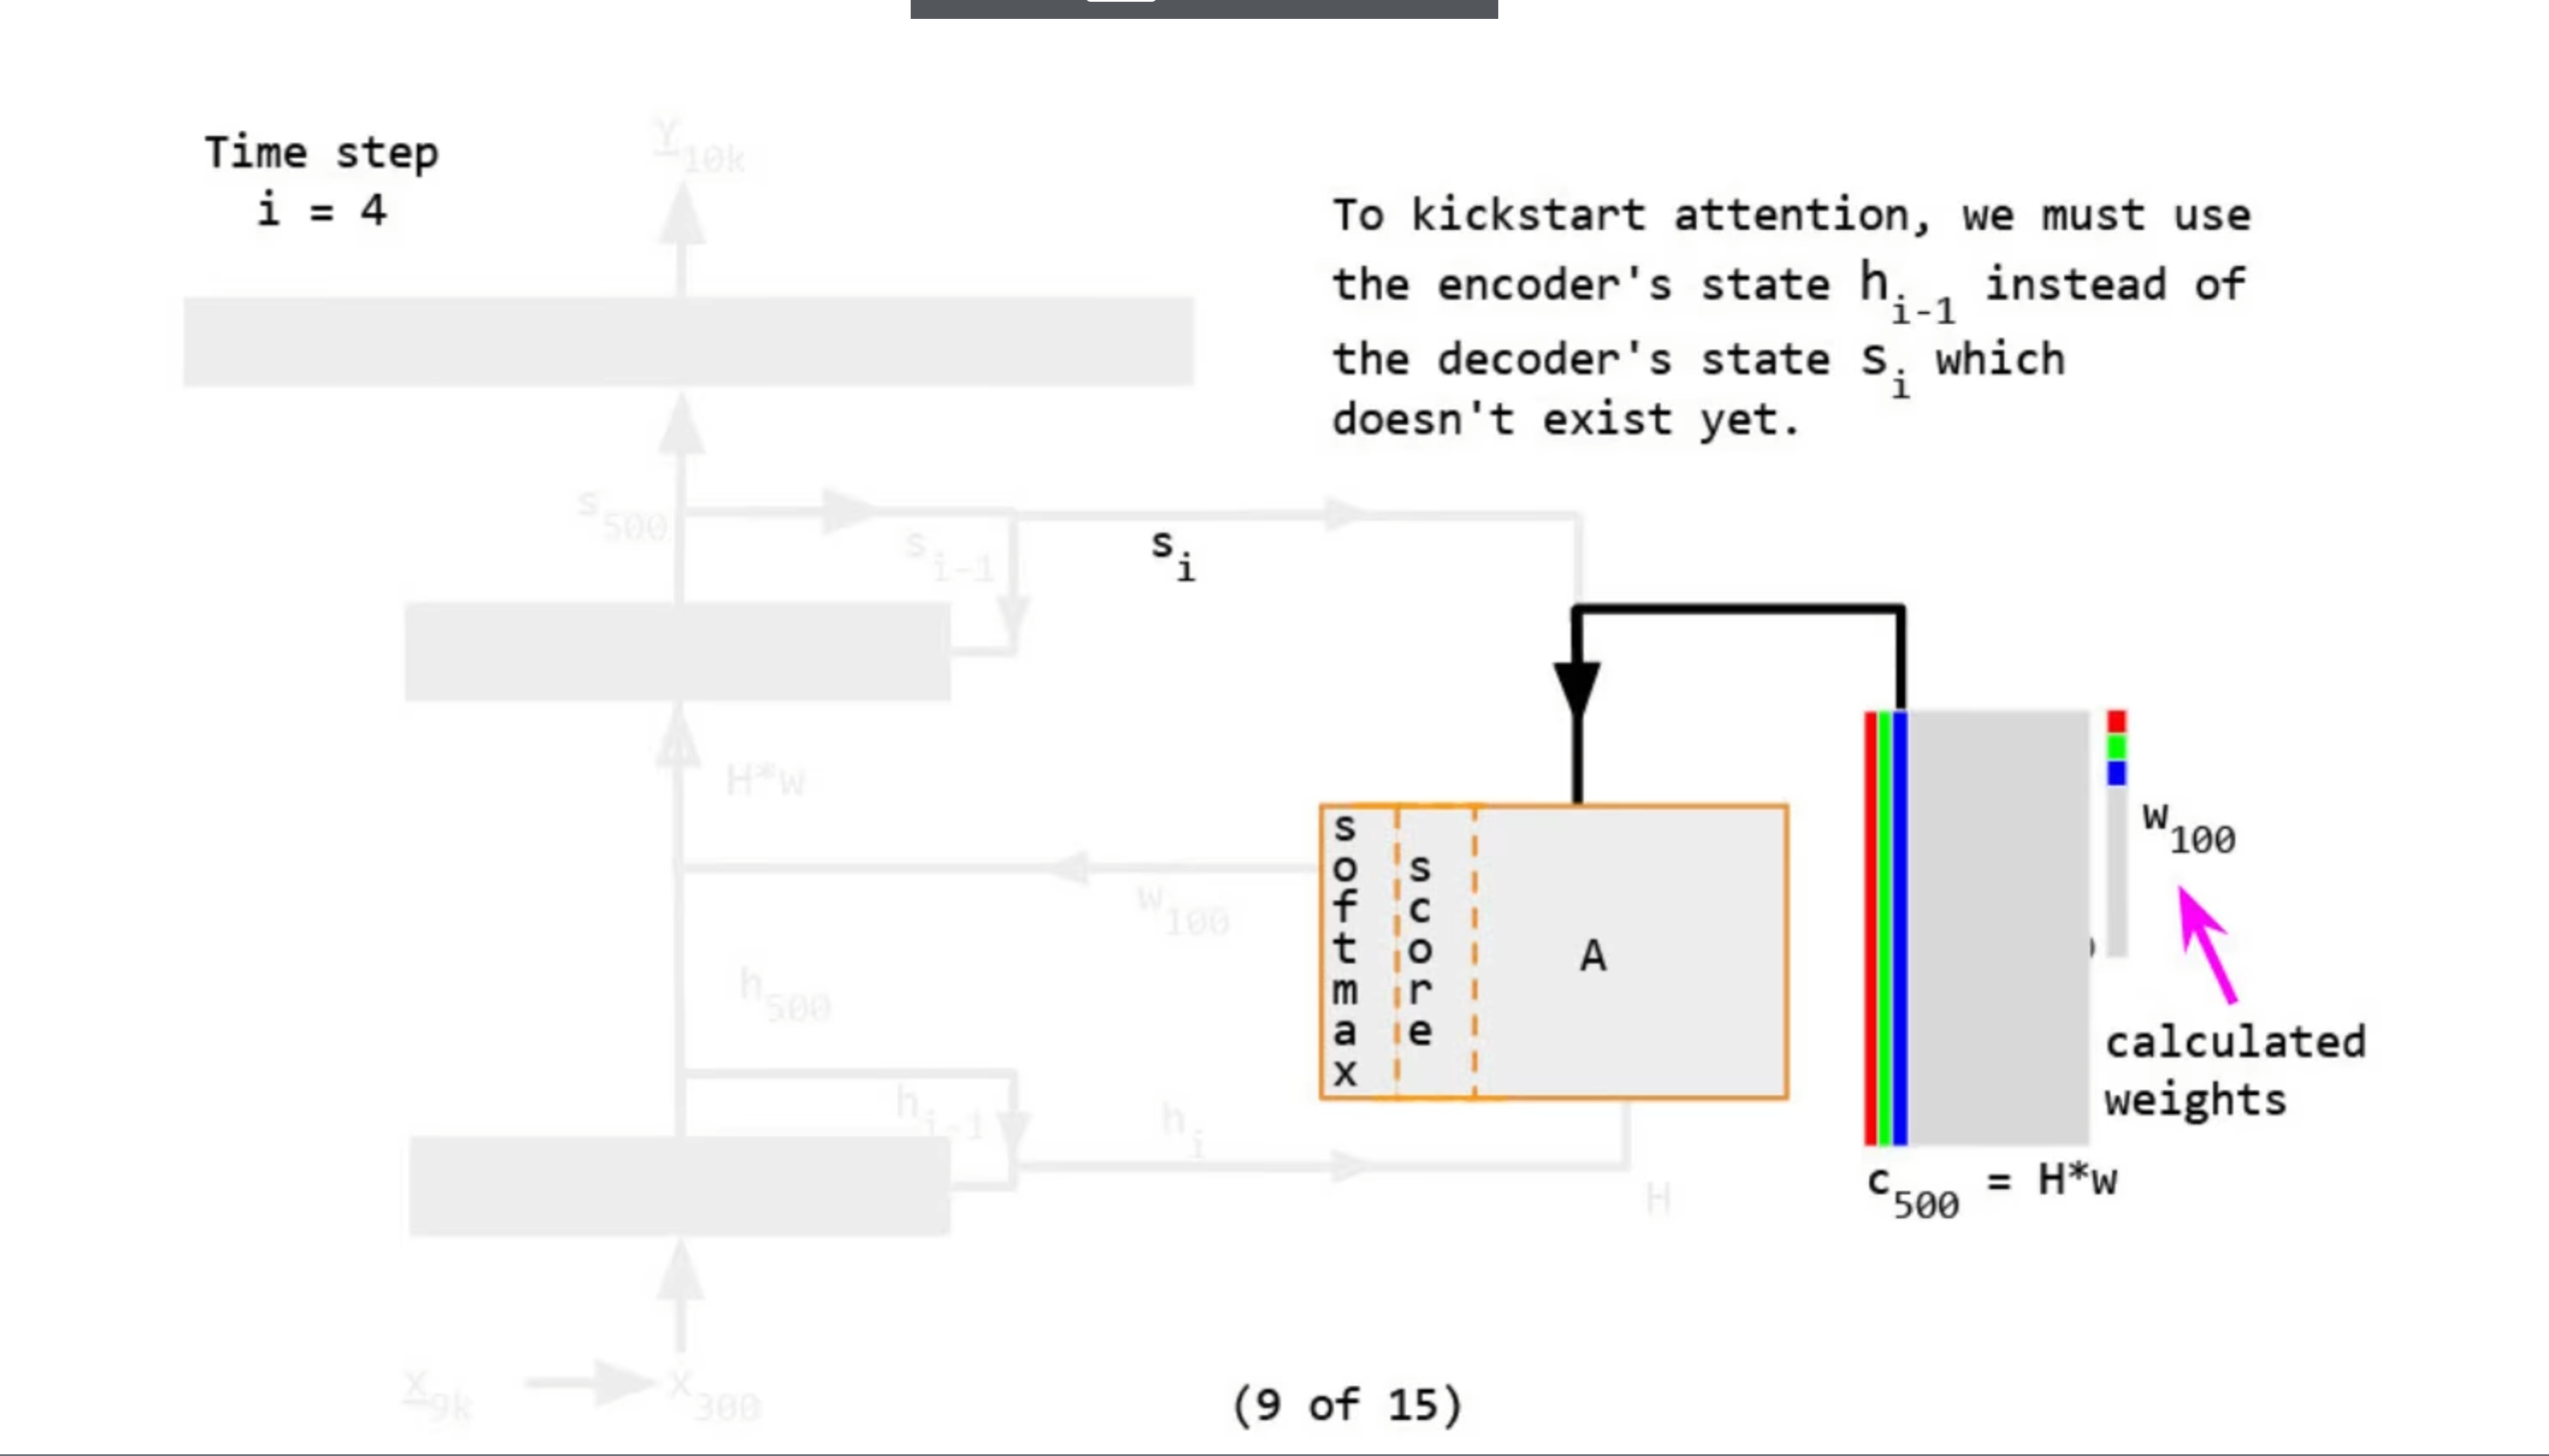
\includegraphics[width=1.3\textwidth]{./translation/9.jpg}
  \end{minipage}
\end{figure}
\end{frame}

\begin{frame}{A language translation example}
\begin{figure}
  \begin{minipage}[b]{0.4\textwidth}
    \par\medskip
    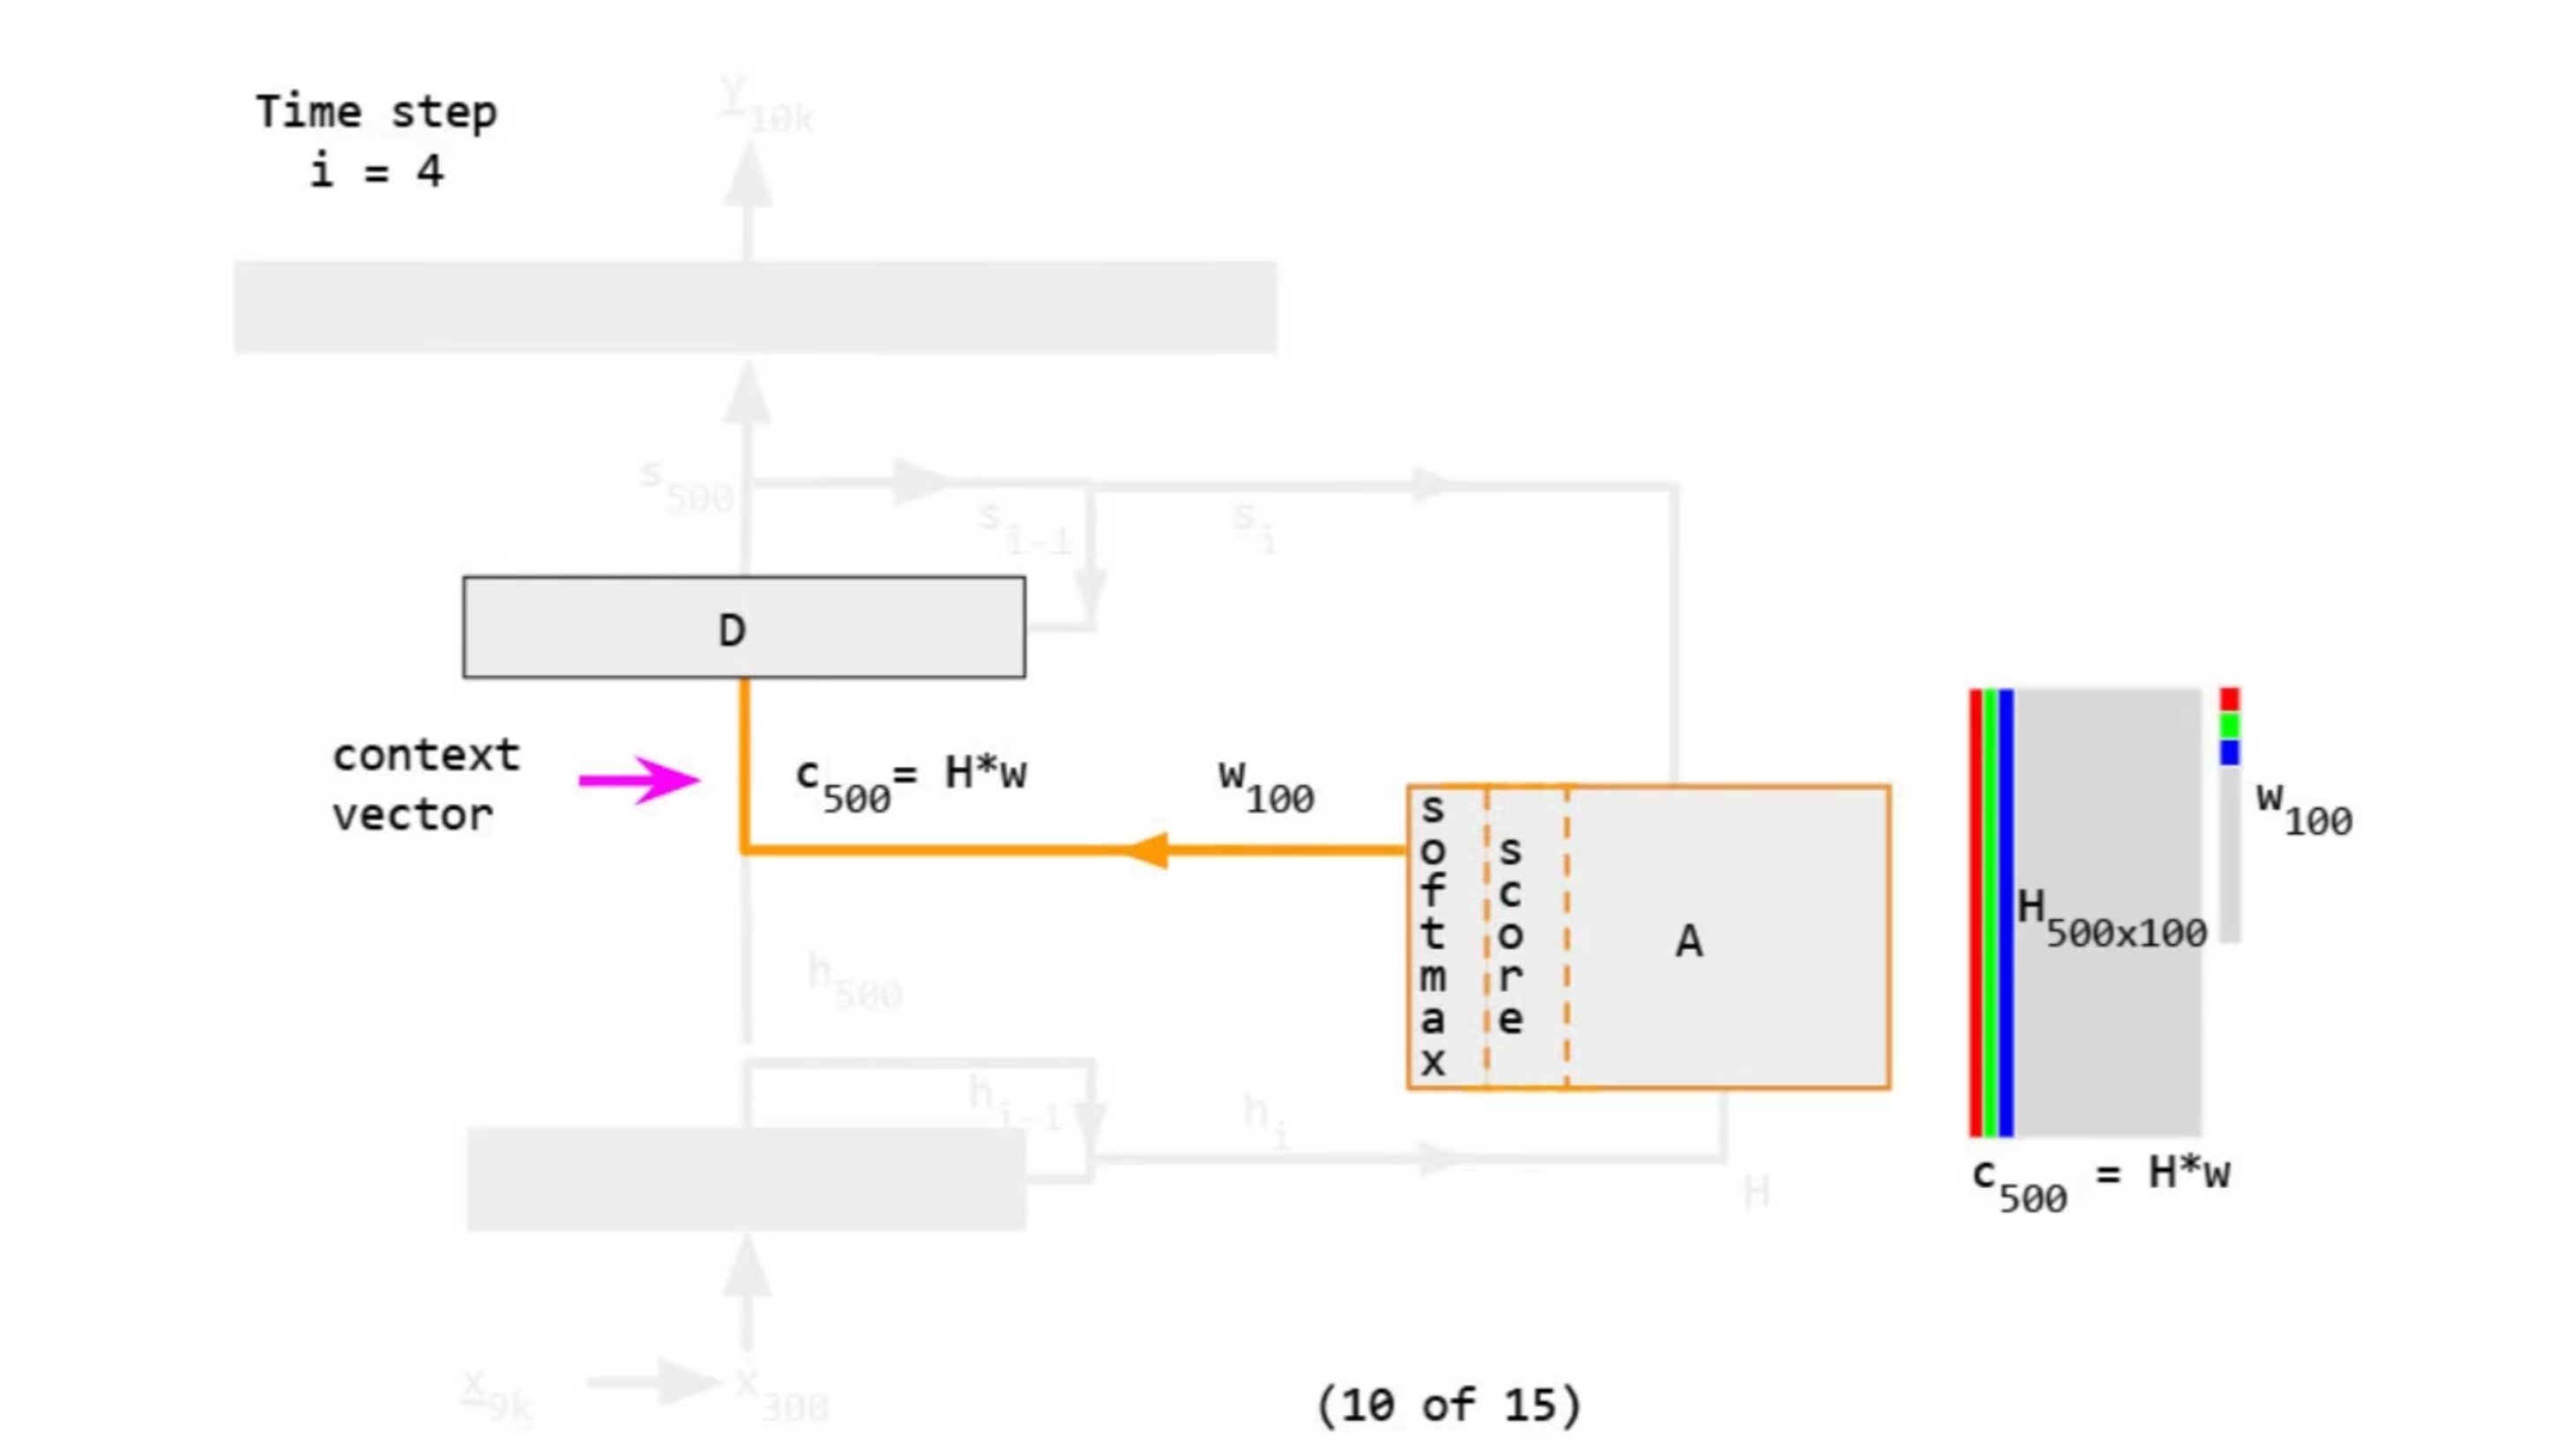
\includegraphics[width=1.3\textwidth]{./translation/10.jpg}
  \end{minipage}
  \hfill
  \begin{minipage}[b]{0.4\textwidth}
    \par\medskip
    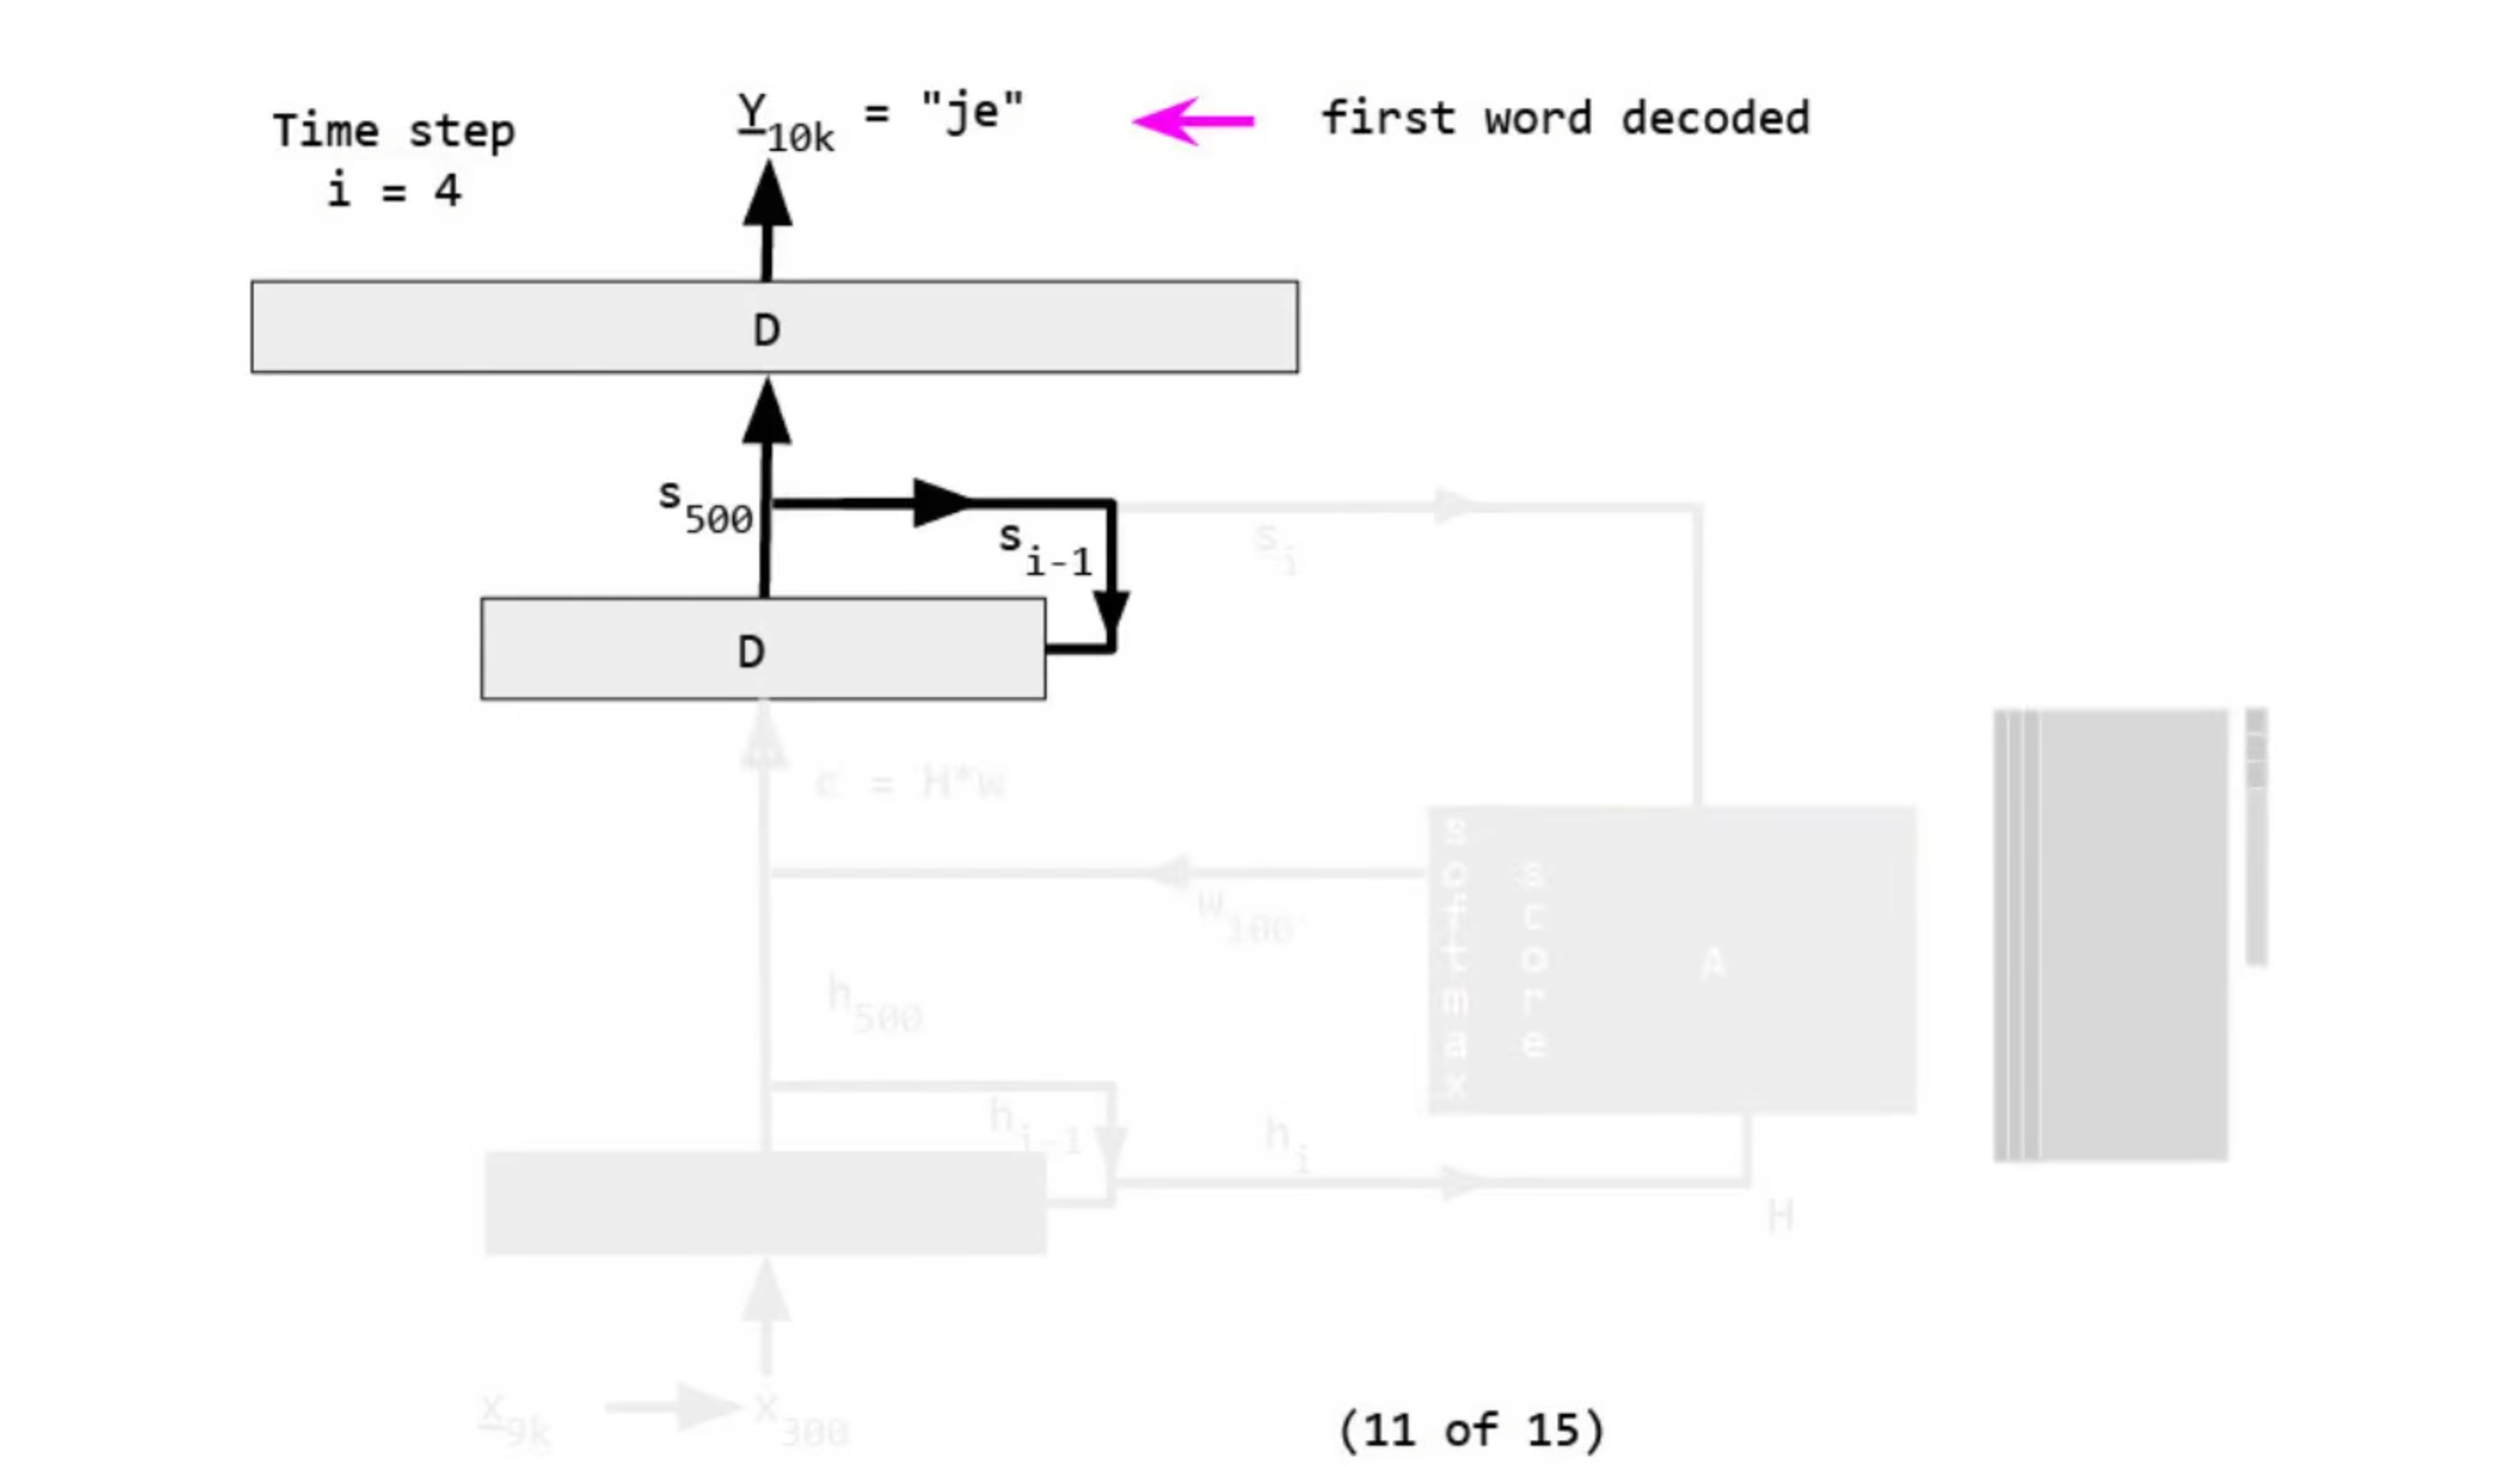
\includegraphics[width=1.3\textwidth]{./translation/11.jpg}
  \end{minipage}
  \begin{minipage}[b]{0.4\textwidth}
    \par\medskip
    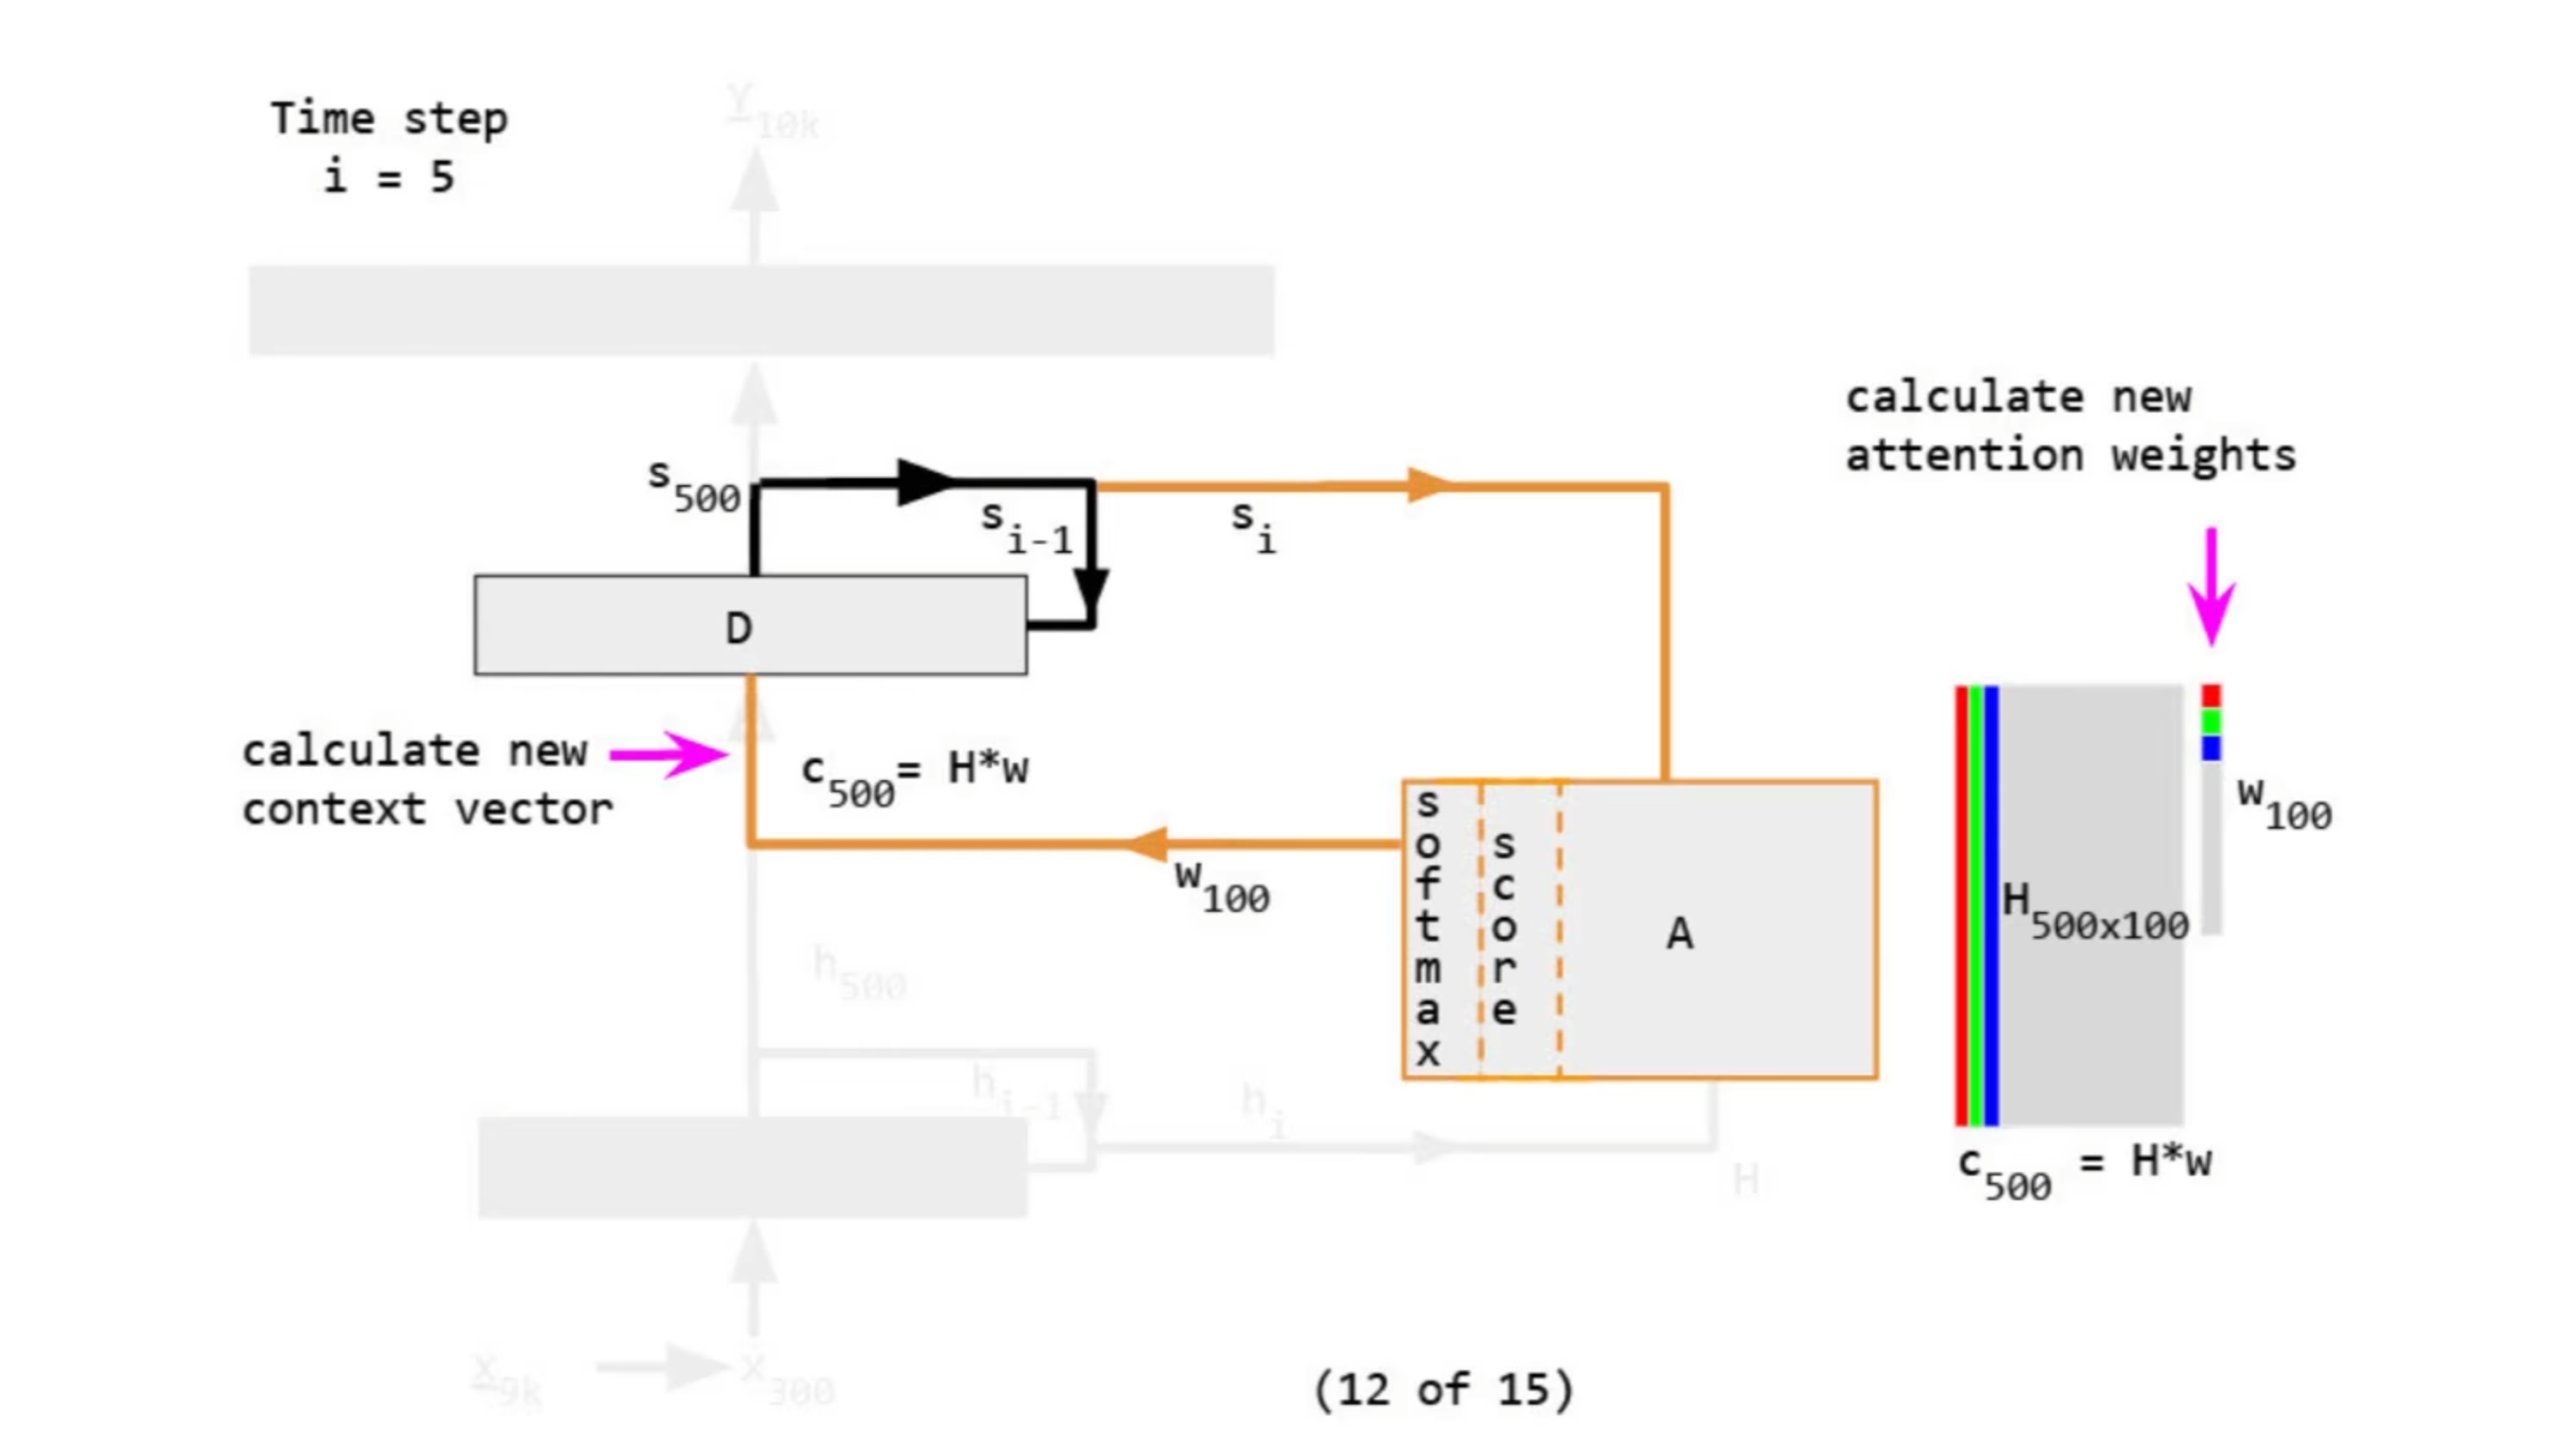
\includegraphics[width=1.3\textwidth]{./translation/12.jpg}
  \end{minipage}
\end{figure}
\end{frame}

\begin{frame}{A language translation example}
\begin{figure}
  \begin{minipage}[b]{0.4\textwidth}
    \par\medskip
    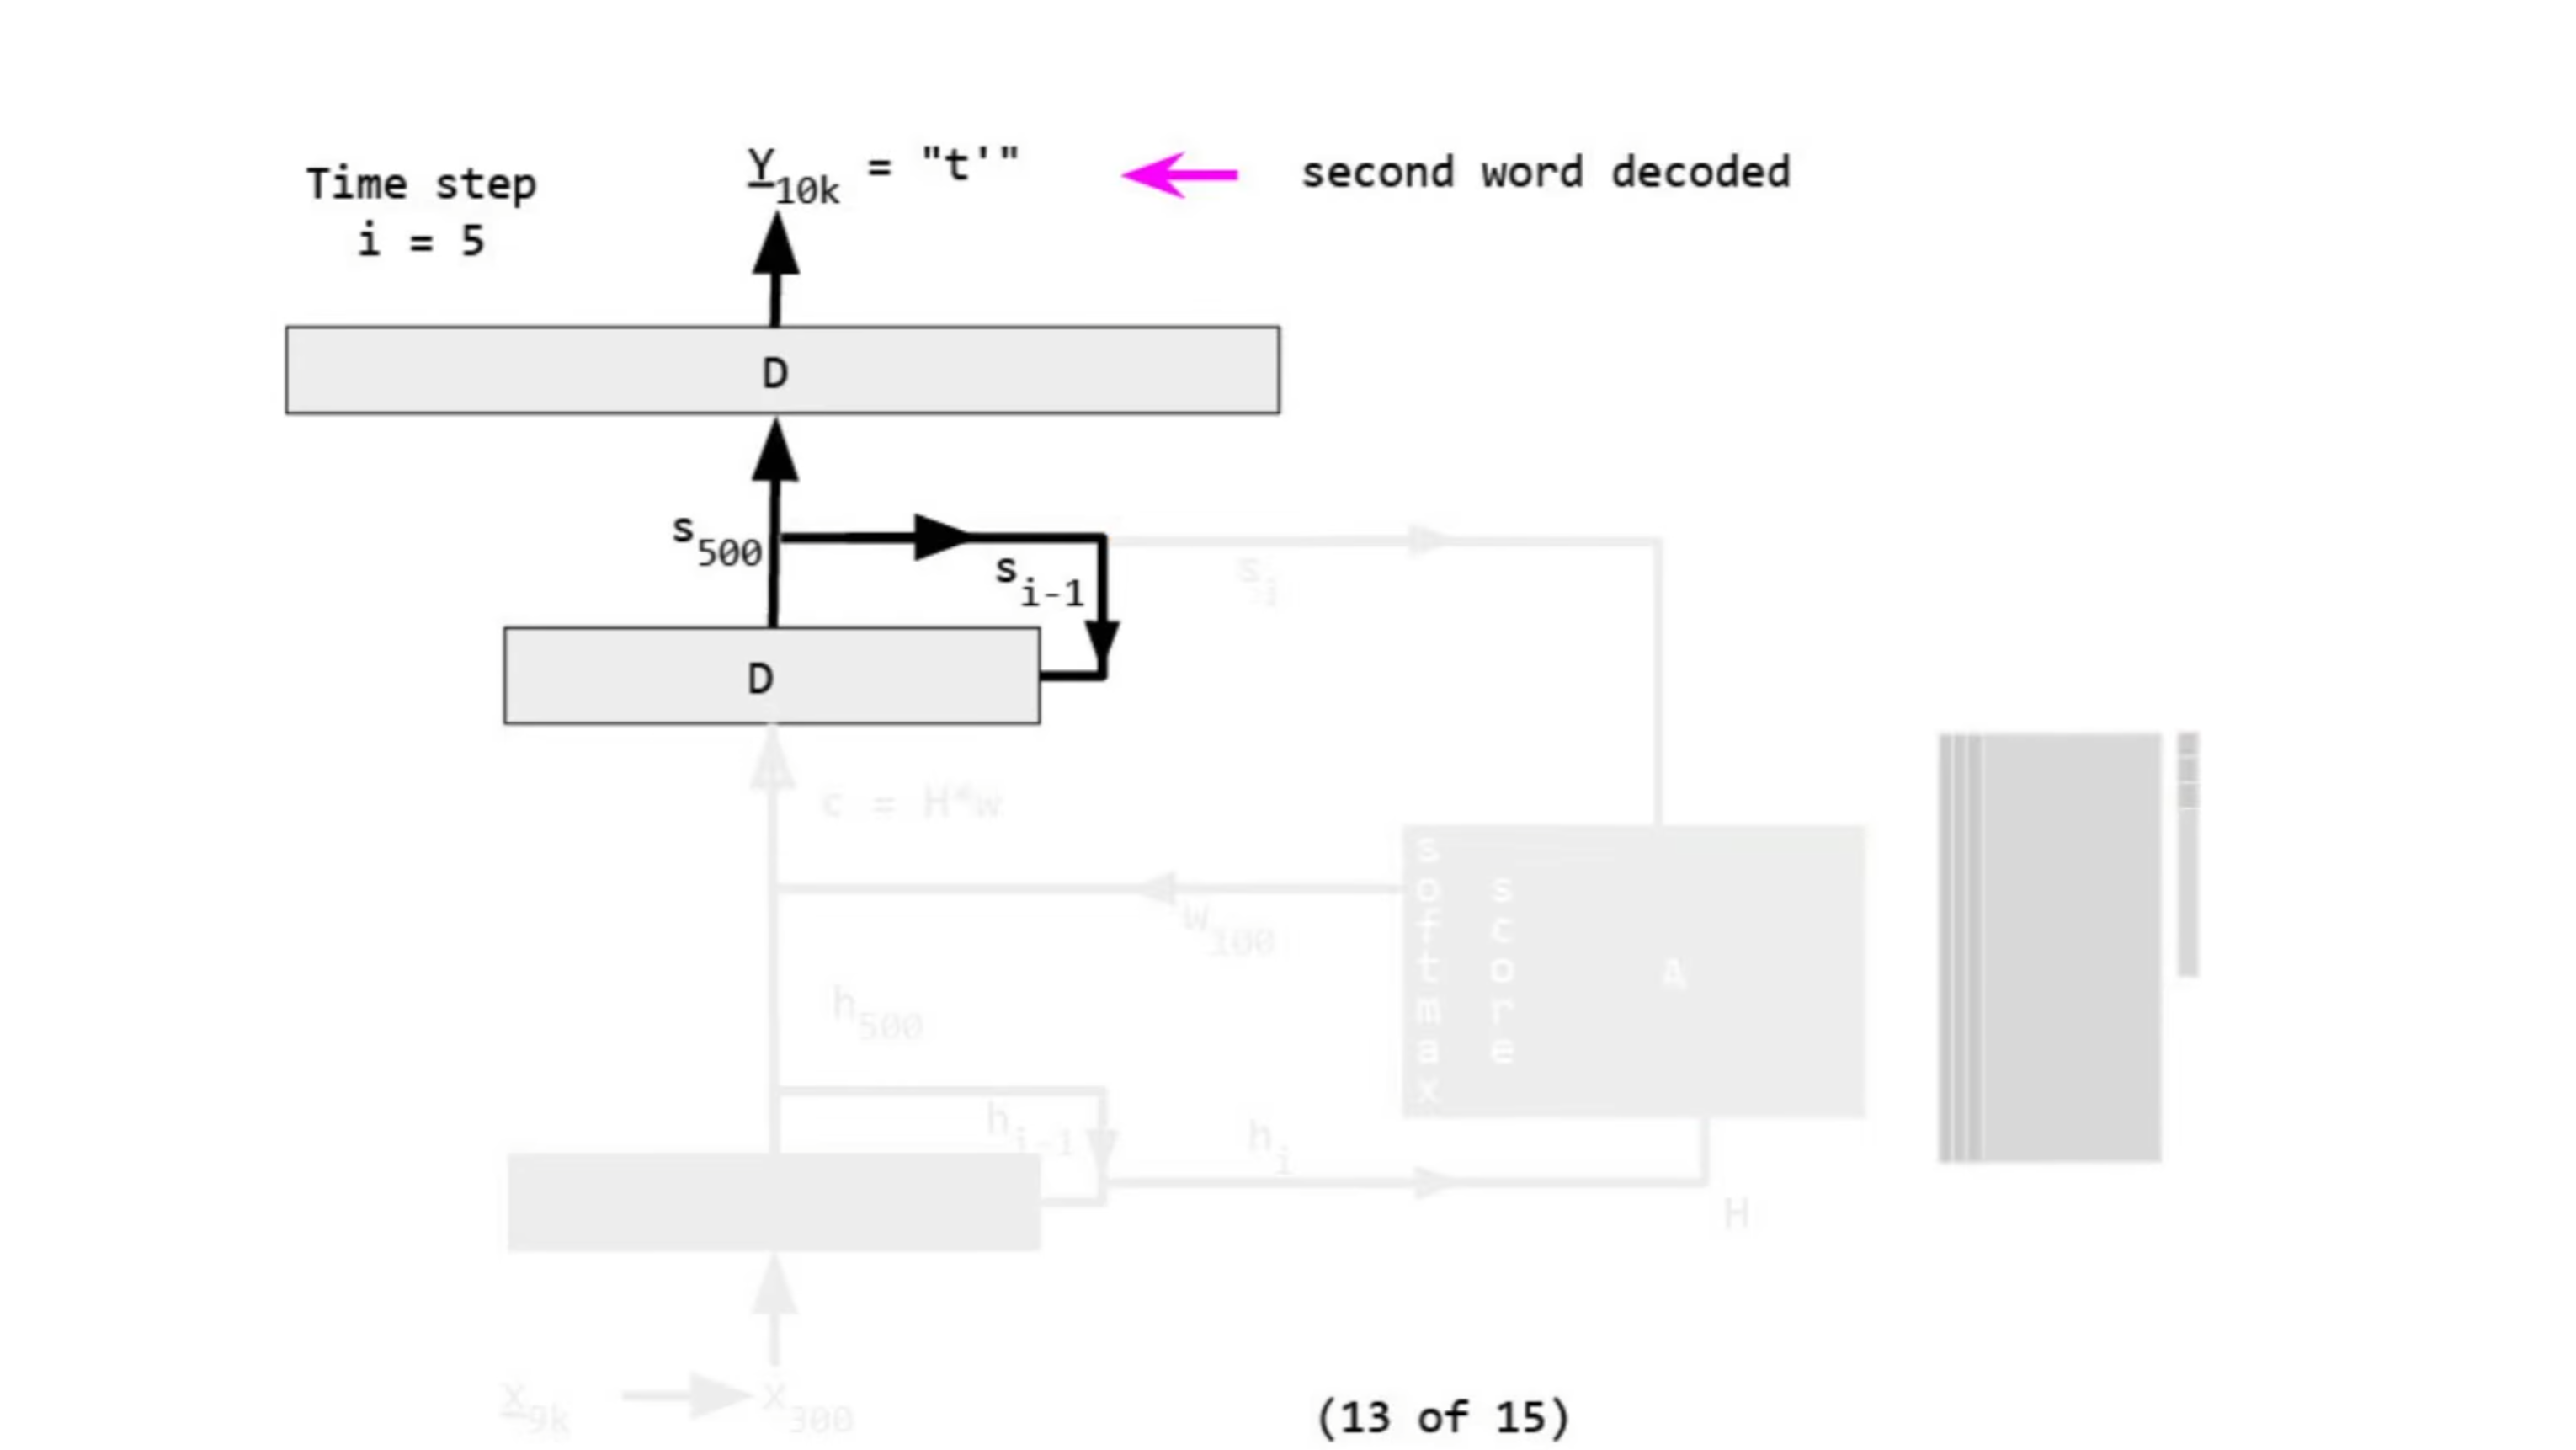
\includegraphics[width=1.3\textwidth]{./translation/13.png}
  \end{minipage}
  \hfill
  \begin{minipage}[b]{0.4\textwidth}
    \par\medskip
    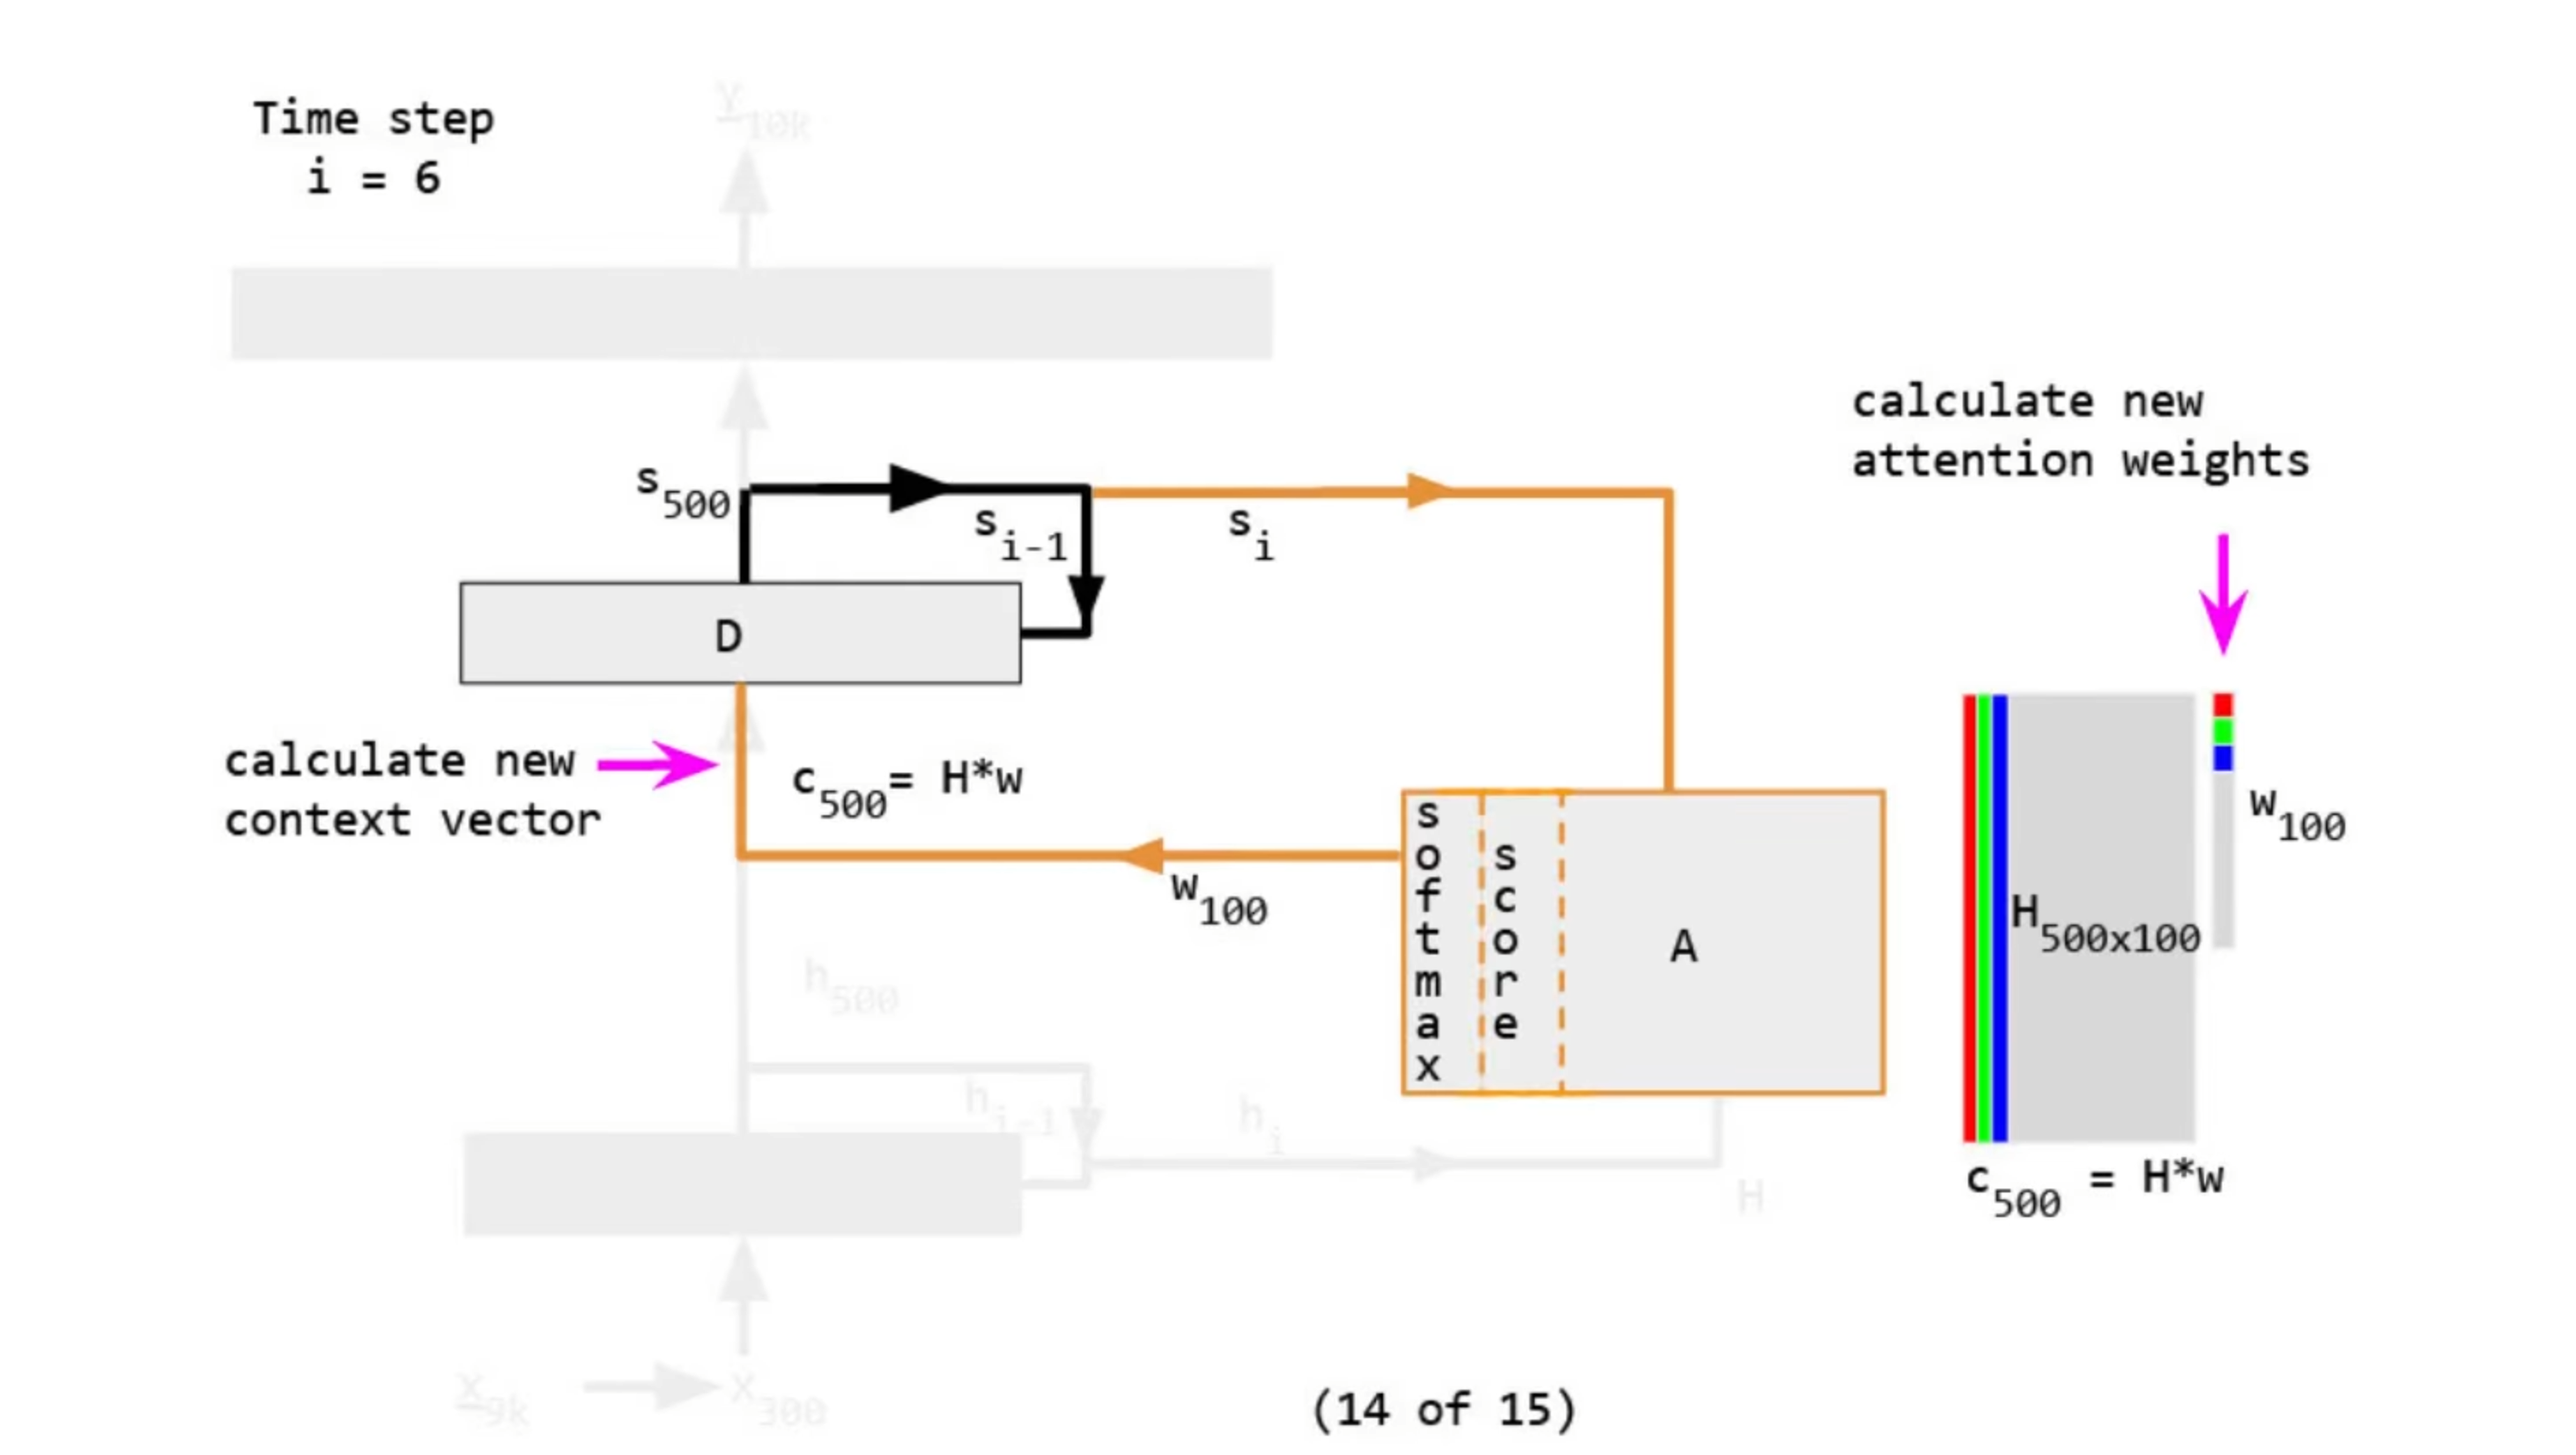
\includegraphics[width=1.3\textwidth]{./translation/14.jpg}
  \end{minipage}
  \begin{minipage}[b]{0.4\textwidth}
    \par\medskip
    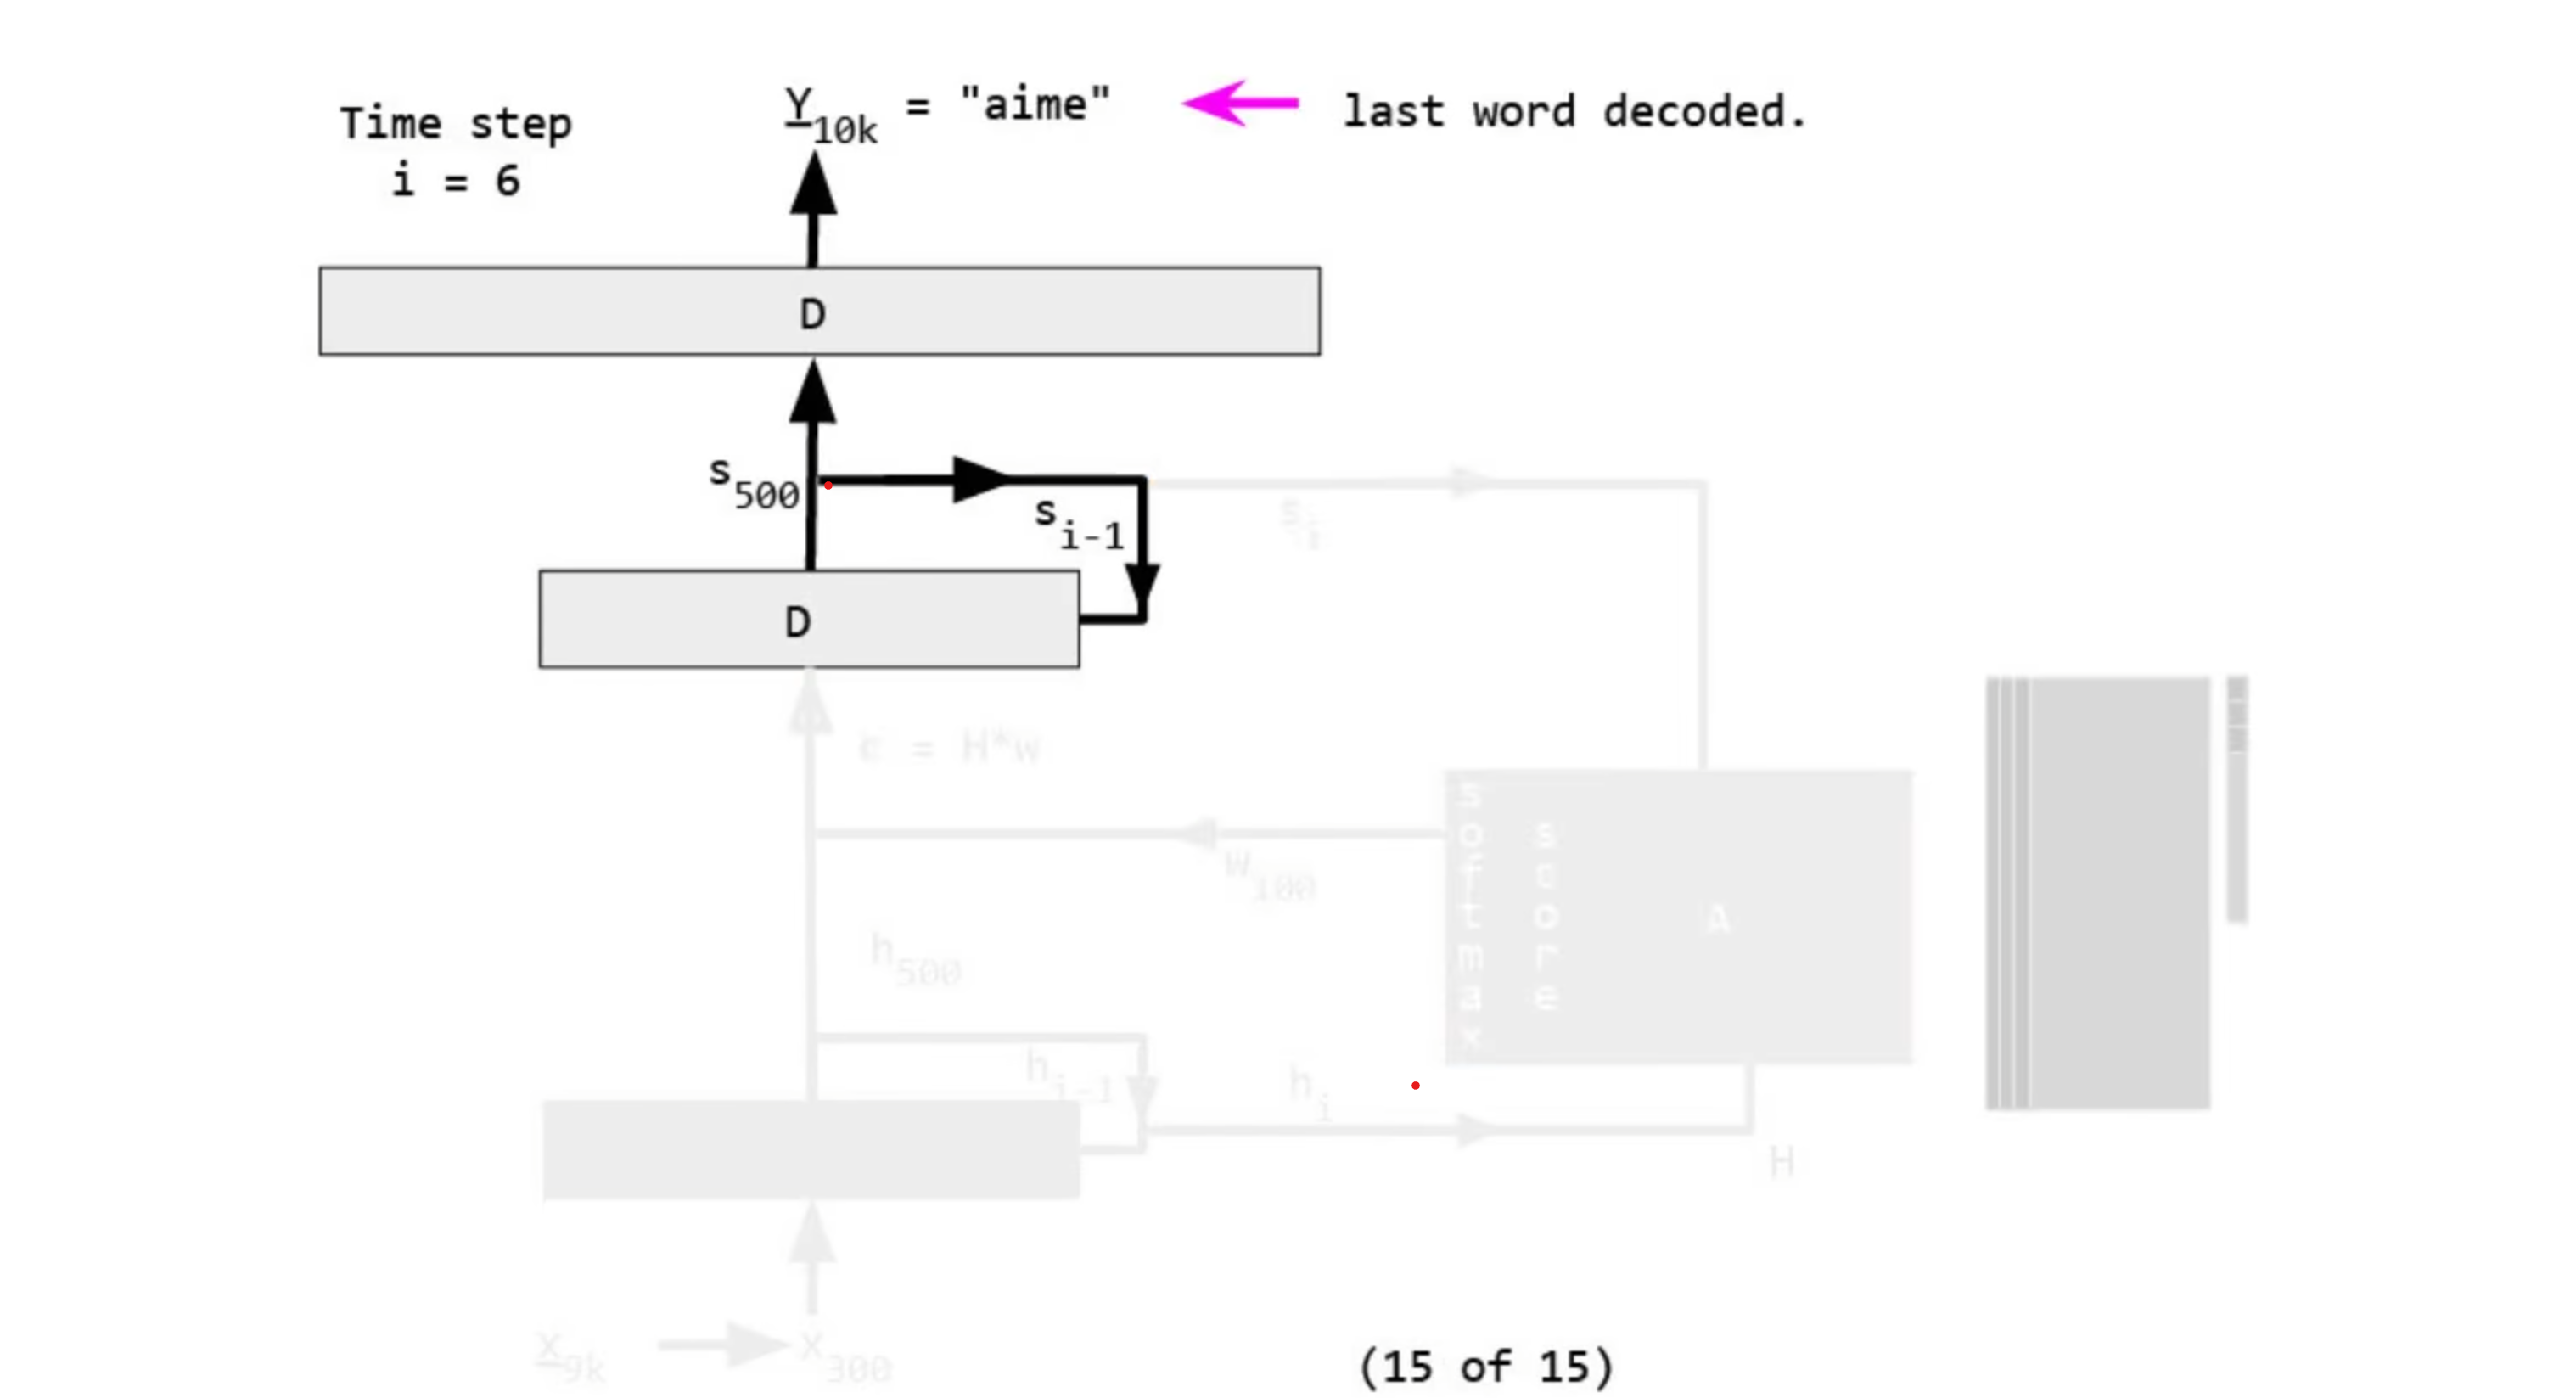
\includegraphics[width=1.3\textwidth]{./translation/15.png}
  \end{minipage}
\end{figure}
\end{frame}

\begin{frame}{Training Details and Experimental Setup}
  \begin{itemize}
    \item Hardware Details:
      \subitem{Trained on 8 NVIDIA P100 GPU}
      \subitem{The big models were trained for 300,000 steps (3.5 days)}
    \item Datasets:
      \subitem{Trained on WMT 2014 English-to-German translation task}
      \subsubitem{4.5 million sentence pairs}
      \subitem{Trained on WMT 2014 English-to-French translation task}
      \subsubitem{36 million sentences}
  \end{itemize}
\end{frame}

\begin{frame}{Experimental Results}
  \begin{itemize}
    \item New single-model state-of-the-art BLEU score of 41.0 for English-to-French
    \item 28.4 BLEU on the WMT 2014 English-to-German translation task
  \end{itemize}
  \center
  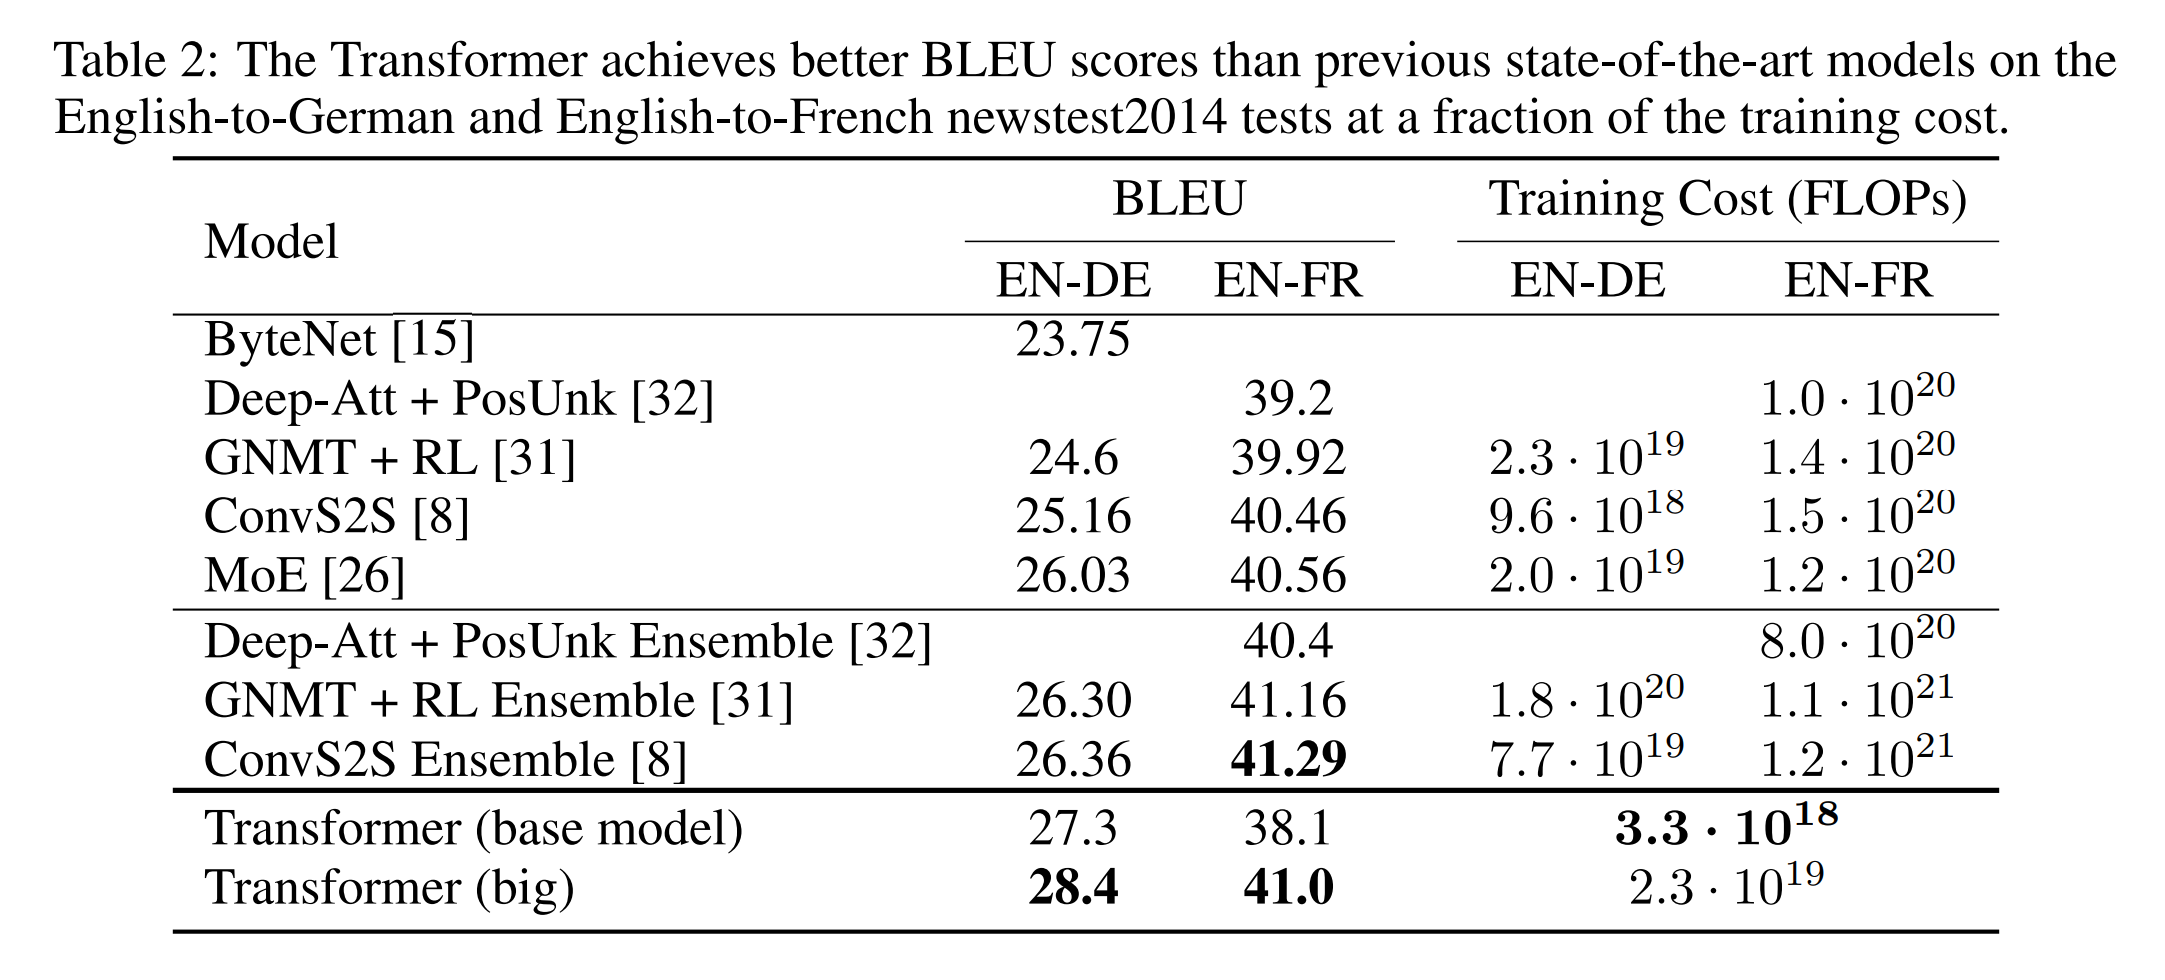
\includegraphics[width=0.8\textwidth]{result.png}
\end{frame}

\begin{frame}{Conclusion}
  \begin{itemize}
    \item Extremely efficient for parallelization (great for GPU)
    \item State-of-the-art performance
    \item Authors state desire to “investigate local, restricted attention mechanisms to efficiently handle large inputs and outputs such as images, audio and video”
  \end{itemize}
\end{frame}

\begin{frame}{Future Work for Reading}
  \begin{itemize}
    \item NLP
      \subitem{BERT - Bidirectional Transformers for NLP}
      \subsubitem{https://arxiv.org/abs/1810.04805}
      \subitem{RoBERTa}
      \subsubitem{https://arxiv.org/abs/1907.11692}
      \subitem{GPT-3: Its Nature, Scope, Limits, and Consequences}
      \subsubitem{https://link.springer.com/content/pdf/10.1007/s11023-020-09548-1.pdf}
    \item Computer Vision:
      \subitem{Vision Transformer (ViT)}
      \subitem{Swin Transformers}
  \end{itemize}
\end{frame}

\nocite{*}
\begin{frame}{References}
    \printbibliography
\end{frame}


\begin{frame}{}
  \centering \Huge
  \emph{Thanks for listening!}
\end{frame}

\end{document}



